\documentclass[a4paper,12pt]{book}

\usepackage{estilosbase}
\usepackage{textcomp}
\usepackage{multirow}
\usepackage{graphicx}
\usepackage{subcaption}
\usepackage{siunitx}

\headsep = 27 pt
\clearpage{\pagestyle{empty}\cleardoublepage}

\begin{document}
\selectlanguage{spanish}
\renewcommand{\labelitemi}{$\bullet$}
\renewcommand{\labelitemii}{$\diamond$}
\renewcommand{\figurename}{Figura}
\renewcommand{\listfigurename}{Índice de figuras}
\renewcommand{\tablename}{Tabla}
\renewcommand{\listtablename}{Índice de tablas}
\newcommand{\icontext}[3]{\raisebox{-#1\height}{\includegraphics[scale=#2]{#3}}}
\newcommand{\quotes}[1]{``#1''}
\setcounter{secnumdepth}{5} 

% Este archivo es parte de la memoria del proyecto fin de carrera
% de Manuel López Urbina. Protegida bajo la licencia GFDL.
% Para más información, la licencia completa viene incluida en el
% fichero fdl-1.3.tex
% Fuente tomada del PFC 'libgann' de Francisco Javier Vázquez Púa.
% Fuente tomada de la plantilla LaTeX para
% la realización de Proyectos Final de Carrera de Pablo Recio Quijano.
% Copyright (C) 2009 Pablo Recio Quijano

% Copyright (C) 2017 Manuel López Urbina

\pagestyle{empty}
\begin{titlepage}

  \begin{center}

    
\includegraphics[scale=0.2]{inicio/logo_uca.png} \\

    \vspace{2.0cm}

    \LARGE{\textbf{ESCUELA SUPERIOR DE INGENIERÍA}} \\

    \vspace{1.0cm}

    \Large{\textbf{MÁSTER UNIVERSITARIO EN INVESTIGACIÓN EN INGENIERÍA DE SISTEMAS Y DE LA COMPUTACIÓN}} \\

    \vspace{3.0cm}

    \Large{\textbf{ Multi Sensor Robot System (SensorRS), Vehículo robótico multisensorial de exploración controlado por wifi basado en Arduino y Raspberry Pi. }} \\

    \vspace{3.0cm}

    \normalsize{Manuel López Urbina \\
    Director: Arturo Morgado Estévez }\\

    \vspace{1.5cm}
    Cádiz, \today

  \end{center}
\end{titlepage}



\cleardoublepage

% Este archivo es parte de la memoria del proyecto fin de carrera
% de Manuel López Urbina. Protegida bajo la licencia GFDL.
% Para más información, la licencia completa viene incluida en el
% fichero fdl-1.3.tex
% Fuente tomada del PFC 'libgann' de Francisco Javier Vázquez Púa.
% Fuente tomada de la plantilla LaTeX para
% la realización de Proyectos Final de Carrera de Pablo Recio Quijano.

% Copyright (C) 2018 Manuel López Urbina

\pagestyle{empty}
\begin{center}

  
\includegraphics[scale=0.2]{inicio/logo_uca.png} \\

  \vspace{2.0cm}

  \Large{ESCUELA SUPERIOR DE INGENIERÍA} \\

  \vspace{1.0cm}

  \large{MÁSTER UNIVERSITARIO EN INVESTIGACIÓN EN INGENIERÍA DE SISTEMAS Y DE LA COMPUTACIÓN} \\
  
  \vspace{2.0cm}

  \large{Multi Sensor Robot System (SensorRS), Vehículo robótico multisensorial de exploración controlado por WiFI basado en Arduino y Raspberry Pi.} \\

  \vspace{1.0cm}

\end{center}

\begin{itemize}
\item \large{Departamento: Ingeniería en Automática, Electrónica, Arquitectura y Redes de Computadores}
\item \large{Director del proyecto: Arturo Morgado Estévez}
\item \large{Autor del proyecto: Manuel López Urbina}
\end{itemize}

\vspace{1.0cm}

\begin{flushright}
  \large{Cádiz, \today} \\

  \vspace{2.5cm}

  \large{Fdo: Manuel López Urbina}
\end{flushright}

\cleardoublepage

\frontmatter
\pagestyle{plain}
% Este archivo es parte de la memoria del proyecto fin de carrera
% de Manuel López Urbina. Protegida bajo la licencia GFDL.
% Para más información, la licencia completa viene incluida en el
% fichero fdl-1.3.tex

% Copyright (C) 2017 Manuel López Urbina

\section{Agradecimientos}
\label{sec:agradecimientos}

Este proyecto significa la culminación de mi carrera, por lo que me gustaría dedicárselo a todas las personas que me han ayudado a conseguir acabarla.\bigskip

En primer lugar me gustaría agradecerle, de igual modo que en el PFC de la Ingeniería Técnica, a mi familia el apoyarme y ayudarme durante estos años,
y el esfuerzo que han hecho para que yo haya podido culminar mi ingeniería.\bigskip

Mención especial para Natalia Luciano, mi pareja, la cual ha estado siempre apoyándome en mis objetivos y tanta paciencia y comprensión me ha mostrado tras tantos días, meses e incluso años de estudio 
y dedicación.\bigskip

Agradecimientos a D. Arturo Morgado por su ayuda y dedicación durante la realización y dirección de este proyecto, así como su carácter amable y servicial que han hecho más ameno el trabajo realizado.\bigskip

También me gustaría agradecérselo a mis compañeros, con los que tantos ratos inolvidables he pasado, y que tanto me han ayudado.\bigskip

Por último quiero dedicarle este proyecto a todos los estudiantes de informática, en especial a todos los amantes del fascinante mundo de la robótica, a los que espero que mi trabajo les sea de utilidad.

\cleardoublepage

\section{Licencia}
\label{sec:licencia}

\bigskip
\bigskip

La aplicación RobotUI es software libre: usted puede redistribuirlo y/o modificarlo bajo los términos de la Licencia Pública General de GNU según lo publicado por la Free Software Foundation, ya sea la versión 3 
de la Licencia, o (a su elección) cualquier versión posterior.\\

Este programa se distribuye con la esperanza de que sea útil, pero SIN NINGUNA GARANTÍA, incluso sin la garantía implícita de COMERCIALIZACIÓN o IDONEIDAD PARA UN PROPÓSITO PARTICULAR. Ver el GNU
General Public License para más detalles.\\

Este documento ha sido liberado bajo Licencia GFDL 1.3 (GNU Free Documentation License). Se incluyen los términos de la licencia en inglés al final del mismo. Si no es así, 
consulte \href{http://www.gnu.org/licenses/}{GNU Licenses}.\\\bigskip

\begin{quote}
Copyright \copyright~\the\year~ Manuel López Urbina.\bigskip

Permission is granted to copy, distribute and/or modify this document under the terms of the GNU Free Documentation License, Version 1.3 or  any later version published by the Free Software Foundation; with no Invariant Sections, no Front-Cover Texts, and no Back-Cover Texts. A copy of the license is included
in the section entitled "GNU Free Documentation License".
\end{quote}


\cleardoublepage


\cleardoublepage

% Este archivo es parte de la memoria del proyecto fin de carrera
% de Manuel López Urbina. Protegida bajo la licencia GFDL.
% Para más información, la licencia completa viene incluida en el
% fichero fdl-1.3.tex

% Copyright (C) 2018 Manuel López Urbina

\section*{Resumen}
\label{resumen}

Multi Sensor Robot System (SensorRS), Vehículo robótico multisensorial de exploración controlado por WiFI basado en Arduino y Raspberry Pi, es un proyecto robótico elaborado
principalmente con una placa Raspberry Pi interconectada por pueto serie con una placa Arduino. \\

La placa Arduino se ha utilizado para la conexión de una serie de sensores cuya
finalidad es la obtención de variables del entorno como temperatura, humedad, iluminación, etc. Estos parámetros son obtenidos mediante la programación del microcontrolador 
que la placa Arduino incorpora, encargándose, posteriormente, de transmitir información a la placa Raspberry Pi para su procesamiento y envío al servidor web donde se realiza
el seguimiento y control del vehículo y los parámetros obtenidos.\\

La intención principal de este proyecto es la de permitir que usuarios puedan disponer de un vehículo robótico a coste muy reducido y de componentes de fácil adquisición y
de reducido coste. Este vehículo podrá ser utilizado para la realización de labores de exploración de zonas en las que o bien no puede acceder una persona debido al reducido tamaño o 
dificultoso acceso de las áreas a explorar o bien porque alguna situación peligrosa lo impida. En resumidas cuentas un vehículo robótico con un amplio sistema de telemetría incorporado.\\

Dicho sistema es configurado en la aplicación web RobotUI para permitir sus control por parte de otros usuarios. RobotUI incorpora un asistente mediante el cual, cualquier usuario 
sin conocimientos previos de programación, pueda elaborar una interfaz para el control de su dispositivo robótico personalizada y adaptada a sus necesidades de control 
y a las características del dispositivo en cuestión.\\

Dicha interfaz permitirá realizar el control de los mencionados dispositivos además de permitir que otros usuarios entren en las salas o canales donde podrán visualizar el manejo 
que realiza un usuario de su robot en tiempo real donde obtendrán en todo momento las imágenes captadas junto con los diferentes comandos accionados por el usuario 
que está realizando el control.\\

Con todo ello, lo que se busca es crear un sistema robótico controlable por el usuario y que transmita información en tiempo real destinado a la exploración de áreas peligrosas y 
de coste reducido.\\

\textbf{Palabras clave:} Internet, aplicación web, robótica, robots, interfaz de usuario, streaming de vídeo, control remoto, tiempo real, Raspberry Pi, Arduino, sensores, comunicación serie,
telemetría.\\

\cleardoublepage


\frontmatter

%% Este archivo es parte de la memoria del proyecto fin de carrera
% de Manuel López Urbina. Protegida bajo la licencia GFDL.
% Para más información, la licencia completa viene incluida en el
% fichero fdl-1.3.tex

% Copyright (C) 2017 Manuel López Urbina

\section{Agradecimientos}
\label{sec:agradecimientos}

Este proyecto significa la culminación de mi carrera, por lo que me gustaría dedicárselo a todas las personas que me han ayudado a conseguir acabarla.\bigskip

En primer lugar me gustaría agradecerle, de igual modo que en el PFC de la Ingeniería Técnica, a mi familia el apoyarme y ayudarme durante estos años,
y el esfuerzo que han hecho para que yo haya podido culminar mi ingeniería.\bigskip

Mención especial para Natalia Luciano, mi pareja, la cual ha estado siempre apoyándome en mis objetivos y tanta paciencia y comprensión me ha mostrado tras tantos días, meses e incluso años de estudio 
y dedicación.\bigskip

Agradecimientos a D. Arturo Morgado por su ayuda y dedicación durante la realización y dirección de este proyecto, así como su carácter amable y servicial que han hecho más ameno el trabajo realizado.\bigskip

También me gustaría agradecérselo a mis compañeros, con los que tantos ratos inolvidables he pasado, y que tanto me han ayudado.\bigskip

Por último quiero dedicarle este proyecto a todos los estudiantes de informática, en especial a todos los amantes del fascinante mundo de la robótica, a los que espero que mi trabajo les sea de utilidad.

\cleardoublepage

\section{Licencia}
\label{sec:licencia}

\bigskip
\bigskip

La aplicación RobotUI es software libre: usted puede redistribuirlo y/o modificarlo bajo los términos de la Licencia Pública General de GNU según lo publicado por la Free Software Foundation, ya sea la versión 3 
de la Licencia, o (a su elección) cualquier versión posterior.\\

Este programa se distribuye con la esperanza de que sea útil, pero SIN NINGUNA GARANTÍA, incluso sin la garantía implícita de COMERCIALIZACIÓN o IDONEIDAD PARA UN PROPÓSITO PARTICULAR. Ver el GNU
General Public License para más detalles.\\

Este documento ha sido liberado bajo Licencia GFDL 1.3 (GNU Free Documentation License). Se incluyen los términos de la licencia en inglés al final del mismo. Si no es así, 
consulte \href{http://www.gnu.org/licenses/}{GNU Licenses}.\\\bigskip

\begin{quote}
Copyright \copyright~\the\year~ Manuel López Urbina.\bigskip

Permission is granted to copy, distribute and/or modify this document under the terms of the GNU Free Documentation License, Version 1.3 or  any later version published by the Free Software Foundation; with no Invariant Sections, no Front-Cover Texts, and no Back-Cover Texts. A copy of the license is included
in the section entitled "GNU Free Documentation License".
\end{quote}


\cleardoublepage


\cleardoublepage

\tableofcontents
\listoffigures
\mainmatter

\pagestyle{fancy}
\fancyhead[LE,RO]{\rightmark}
\fancyhead[LO,RE]{\slshape \leftmark}
%\fancyroot[C]{\thepage}
  
% Este archivo es parte de la memoria del proyecto fin de carrera
% de Manuel López Urbina. Protegida bajo la licencia GFDL.
% Para más información, la licencia completa viene incluida en el
% fichero fdl-1.3.tex

% Copyright (C) 2018 Manuel López Urbina

\newpage

\chapter{Introducción}
\label{chap:introducción}

La robótica es una rama de la ingeniería, la cual se ocupa del diseño, construcción, operación y uso de robots\footnote{Robot: Máquina automática programable capaz de 
realizar determinadas operaciones de manera autónoma y sustituir a los seres humanos en algunas tareas, en especial las pesadas, repetitivas o peligrosas; puede estar dotada de sensores, 
que le permiten adaptarse a nuevas situaciones.}, así como sistemas informáticos para su control, retroalimentación sensorial y procesamiento de información. Entre las diversas
disciplinas aplicadas a la robótica podemos encontrar: la mecánica, la electrónica, la informática, la inteligencia artificial, la ingeniería de control y la física, entre otras muchas. De lo cual podemos considerar 
la robótica como una ciencia multidisciplinar.\\

Un robot es, por tanto, una máquina capaz de interactuar con su entorno. Si es móvil, a menos que se mueva en un espacio absolutamente acotado y preparado para él, deberá ser
capaz de adaptar sus movimientos y sus acciones de interacción en base a las características físicas de los ambientes con los que se encuentre y los objetos que hay en ellos.\\

Para lograr esta capacidad de adaptación, lo primero que necesitan los robots es tener conocimiento del entorno, resultando ésto absolutamente imprescindible. Para conocer el
entorno los seres vivos recibimos la información mediante los sentidos. Los robots, en infinidad de ocasiones buscando su inspiración en la naturaleza, deben disponer de sistemas que
les permitan saber dónde se encuentran, cómo es el lugar en el que están, a qué condiciones físicas se enfrentan, dónde están los objetos con los que deben interactuar,
sus parámetros físicos, etc.\\

Para esto se utilizan diversos tipos de sensores (o captadores), con un rango de complejidad y sofisticación que varía desde algunos bastante simples a otros con altos niveles de 
sofisticación de hardware y más aún de complejidad de programación.\\

Un sensor\footnote{En el capítulo de conceptos básicos, \ref{sec:sensor-definicion} puede acceder a información más detallada sobre los sensores, descripción, características, etc.}
consta de algún elemento sensible a una magnitud física, como por ejemplo la intensidad o color de la luz, temperatura, presión, magnetismo, humedad, y debe ser capaz,
por su propias características, o por medio de dispositivos intermedios, de transformar esa magnitud física en un cambio eléctrico que se pueda alimentar en un circuito para
que la utilice directamente, o bien, pasando por una etapa previa que la condicione (amplificando, filtrando, etc.). Todo ello para que una vez procesada la señal por el robot
 éste actúe en consecuencia al parámetro recibido.\\

En la actualidad, estos sensores se encuentran presentes en robots de todo tipo. Éstos robots son muy utilizados en plantas de fabricación, montaje y embalaje, en transporte, en exploraciones en la Tierra y en el espacio, cirugía, armamento, investigación en laboratorios y 
en la producción en masa de bienes industriales o de consumo. También resultan de gran utilidad en la resolución de tareas peligrosas, existiendo multitud de aplicaciones como, 
limpieza de residuos tóxicos, minería, búsqueda, rescate de personas y localización de minas terrestres o accidentes nucleares.\\

Por tanto, centrándonos en el área de resolución de tareas peligrosas para las personas, un robot debe cumplir una serie de requerimientos para que cumpla adecuadamente con una serie 
de cometidos:

\begin{itemize}
 \item La movilidad y destreza para maniobrar en zonas con multitud de obstáculos tales como escombros, típicos de las zonas de desastre o catastróficas.
 \item Capacidad de manipulación y utilización de diverso surtido de herramientas diseñadas para los seres humanos.
 \item Capacidad para ser controlado por los seres humanos que hayan tenido poca o ninguna formación robótica.
 \item Autonomía ya sea total o parcial en el nivel de tarea de toma de decisiones sobre la base de los comandos del operador y entradas de los sensores.
\end{itemize}

De todo lo anterior se extrae, por tanto, la necesidad de elaborar un sistema robótico operado por una persona y que permita el análisis del entorno, junto con la posibilidad de controlarlo mediante una 
aplicación software y una conexión a internet. O lo que es lo mismo, un sistema de \texbf{telemetría}\footnote{En el capítulo de conceptos básicos puede acceder a un apartado específico destinado a la telemetría \ref{def:telemetria}}.\\

La telemetría es una tecnología que permite recabar información de un entorno sin necesidad de estar en él presente. 
La información que se desee medir para posteriormente transmitirla puede ser muy variada, según la situación. Desde el punto de vista de la comunicación, la información que se 
transmite es irrelevante, por lo que una vez establecida la forma en la que se envían y se reciben los datos, podremos añadir, reemplazar o modificar los sensores para adaptar el
proyecto tipo desarrollado a un entorno concreto o diferente al inicialmente pensado.\\

Así que dadas las motivaciones existentes y, junto que la programación web y la robótica son temas que causan en mi un especial interés, hicieron que me lanzara a la elaboración de este
proyecto que unifica ambos campos anteriormente citados.\\

Así surgió \emph{SensorRS, Multi-sensor Robot Sysmtem}.\\

\begin{figure}[H]
  \begin{center}
    
\includegraphics[scale=0.8]{imagenes/logotipo_sensor_rs.png}
  \end{center}
  \label{fig:logo}
 \caption{Logo SensorRS \protect\footnotemark.}
\end{figure}

\footnotetext{Logotipo de \emph{SensorRS}, Multi-sensor Robot Sysmtem.}

\emph{Multi Sensor Robot System (SensorRS), Vehículo robótico multisensorial de exploración controlado por WiFI basado en Arduino y Raspberry Pi}, nombre del sistema resultante, será una combinación de un elemento software (aplicación web RobotUI) y hardware (SensorRC, Multisensor
Robot System) surgido como un sistema para sacar el máximo aprovechamiento de la aplicación RobotUI para la que se eleborará un dispositivo robótico de propósito general cuya finalidad es
análisis y exploración del entorno gracias a los sensores incorporados.\\

SensorRS se compone de un vehículo controlado vía WiFi el cual responde a una serie de señales, \emph{comandos}\footnote{ Comando: instrucción u orden que el usuario proporciona a un sistema informático, 
desde la línea de comandos (como una shell) o desde una llamada de programación.}, a los que responde realizando determinadas acciones. Por otra parte también dispone de una cámara para la captura de imágenes.\\

La interfaz de control generada en la aplicación web RobotUI\footnote{ Aplicación anteriormente desarrollada por Manuel López Urbina para el control de dispositivos robóticos de propósito general. Acceso al 
código fuente: \url{https://github.com/lopi87/SAILS-RobotUI}}, se configurará de tal manera que permita el control del vehículo desarrollado en el presente proyecto. 
Esta aplicación permite dar de alta dispositivos robóticos para su control y retransmisión de su funcionamento en vivo con otros usuarios.\\


\begin{figure}[H]
    \centering
    \begin{subfigure}[b]{0.5\textwidth}
        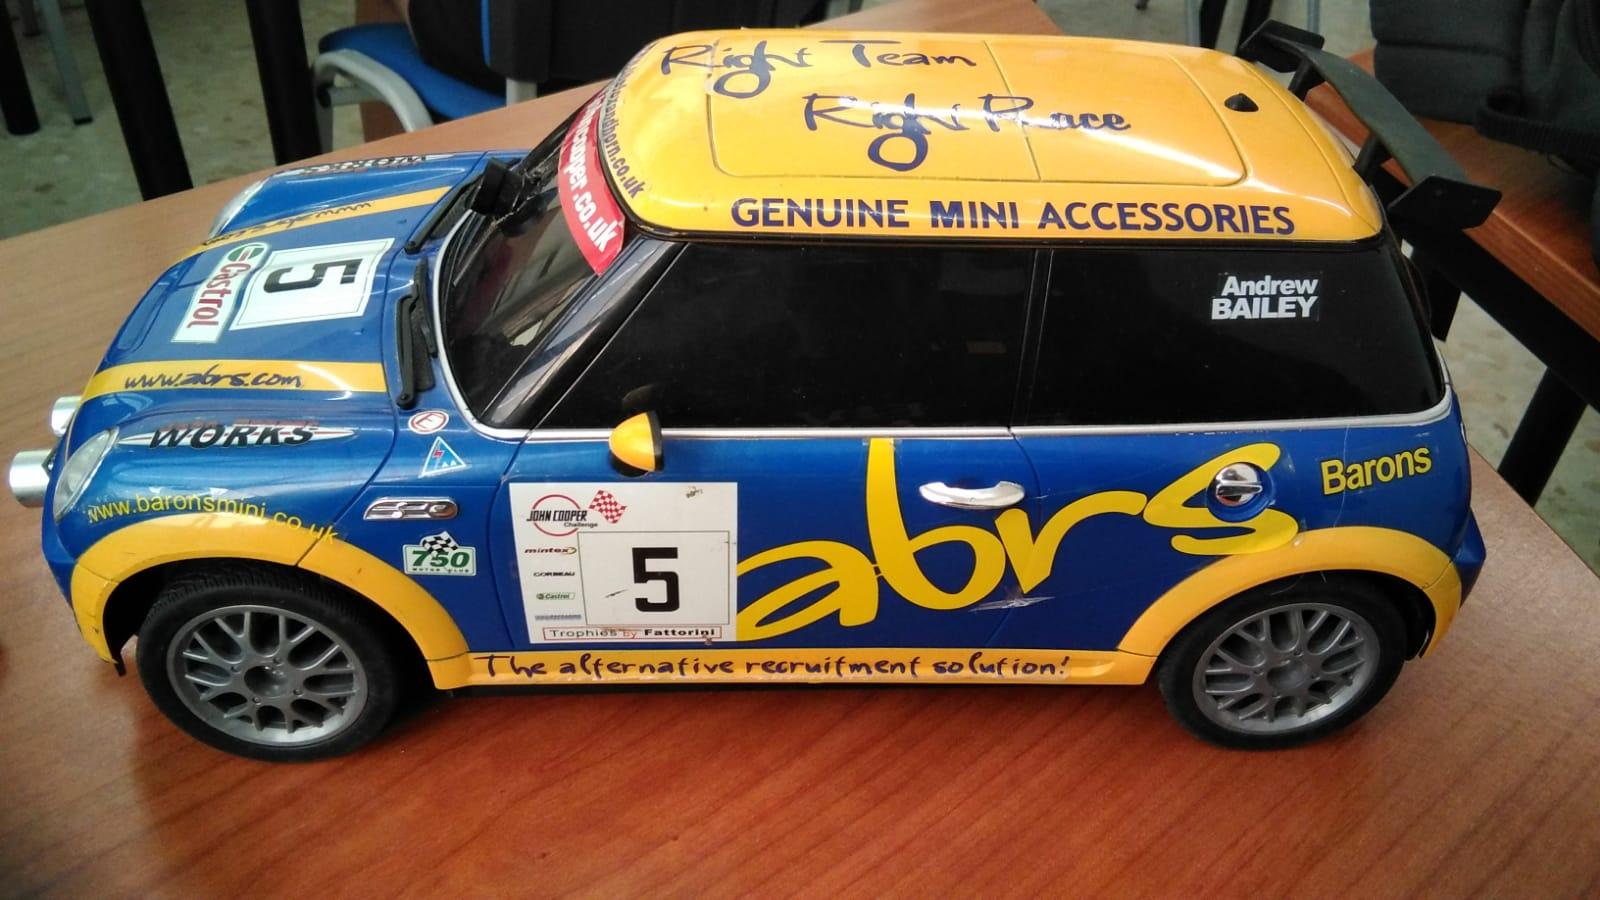
\includegraphics[width=\textwidth]{imagenes/robot/vehiculo_lateral.jpeg}
        \caption{Vista lateral}
        \label{fig:gull}
    \end{subfigure}
    \begin{subfigure}[b]{0.5\textwidth}
        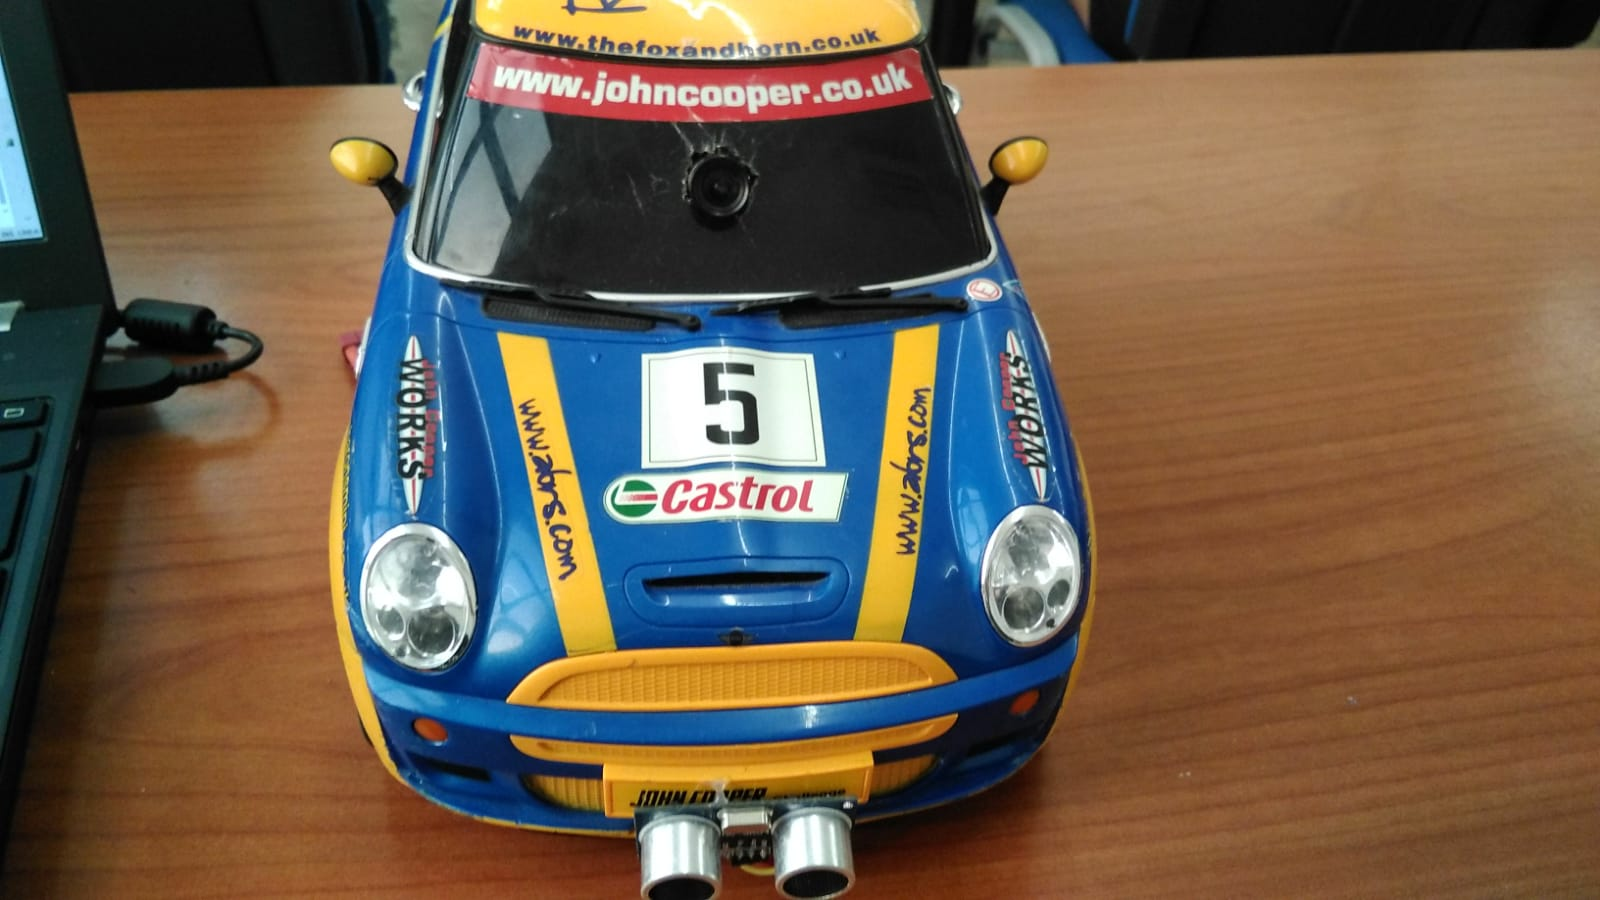
\includegraphics[width=\textwidth]{imagenes/robot/vehiculo_frontal.jpeg}
        \caption{Vista frontal}
        \label{fig:tiger}
    \end{subfigure}
    \begin{subfigure}[b]{0.5\textwidth}
        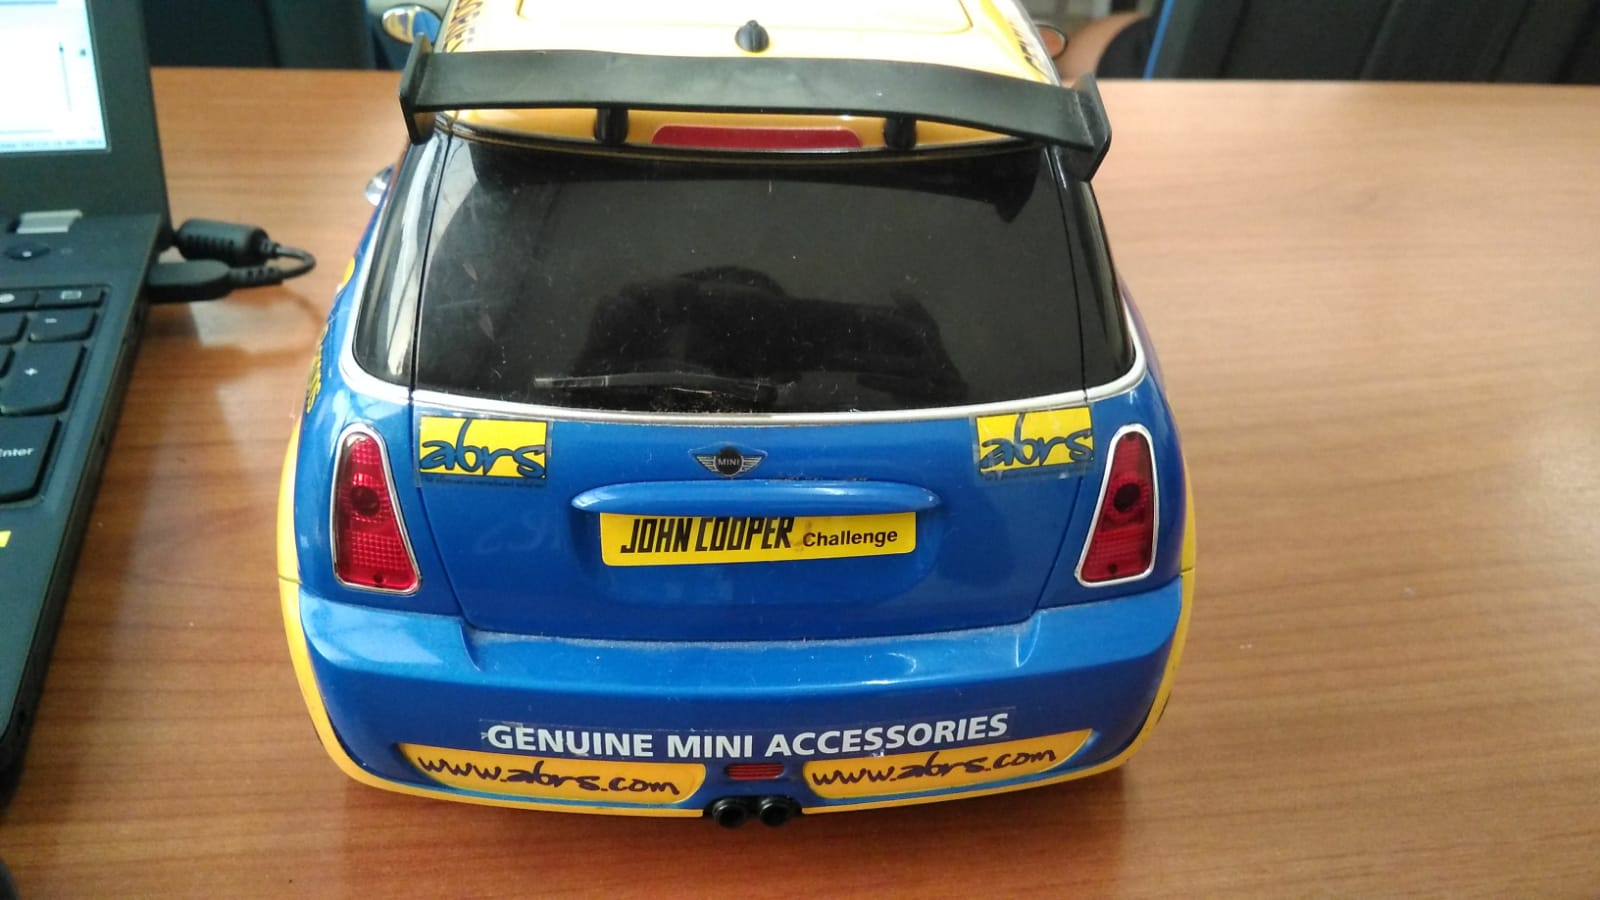
\includegraphics[width=\textwidth]{imagenes/robot/vehiculo_trasera.jpeg}
        \caption{Vista trasera}
        \label{fig:mouse}
    \end{subfigure}
    \caption{Vehículo SensorRS \protect\footnotemark.}\label{fig:animals}
\end{figure}


\footnotetext{Vehículo desarrollado con la finalidad de integrarlo en la aplicación RobotUI. Su desarrollo y características quedan descritas en el capítulo \ref{chap:montaje}.}


\section{Objetivos}
\label{sec:objetivos}

Como hemos visto, se requiere de multitud de conocimientos a la hora de afrontar un proyecto robótico con ciertas garantías. Este proyecto trata de la elaboración 
de un vehículo robótico de fácil construcción mediante la utilización de componentes fácilmente adquiribles y de reducido coste.\\

Dicho robot irá destinado al área de la exploración, buscando, al menos, reducir la exposición de personas a zonas peligrosas ayudando a las labores de rastreo 
o incursión en lugares en principio inalcanzables o de dificultoso acceso.\\

En la presente memoria se abarcará la descripción del diseño, construcción y control de un Robot autómata teledirigido a base de una placa Arduino y Raspberry Pi dotado de multitud de sensores que ayuden a proporcionar 
información del entorno más próximo en el que se encuentra.\\

En lo referente al área de la programación, más concretamente con la programación de microcontroladores\footnote{Un microcontrolador (abreviado μC, UC o MCU) es un circuito integrado programable, capaz de 
ejecutar las órdenes grabadas en su memoria. Está compuesto de varios bloques funcionales, los cuales cumplen una tarea específica. Un microcontrolador incluye en su interior las
tres principales unidades funcionales de una computadora: unidad central de procesamiento, memoria y periféricos de entrada/salida. } permitirá crear un sistema fácilmente escalable
donde agregar nuevos sensores no suponga un elevado esferzo.\\

En definitiva, este proyecto intenta demostrar que sin la necesiad de grandes conocimientos en programación, junto con pequeñas nociones de electrónica básica, que cualquier
persona pueda elaborar un proyecto robótico de similares características. Evitanto que multitud de personas vean que no disponer de grandes conocimientos en la materia sean un
impedimento a la hora de comenzar a desarrollar sus ideas.\\


\section{Acerca de este documento}

El documento se ha sido elaborado en un lenguaje claro y sencillo para permitir que un estudiante universitario de Ingeniería Informática pueda comprender los contenidos sin apenas dificultad añadida.\\

Este documento se organiza en los siguientes capítulos:\\

\begin{itemize}

\item En el capítulo \ref{chap:introducción}, Introducción, se comentan las razones que han motivado la creación de este proyecto, así como el propósito del mismo.

\item En el capítulo \ref{chap:conceptos-básicos}, Conceptos básicos, se incluyen definiciones de aquellos conceptos considerados de interés para la correcta comprensión del contenido de la presente memoria.

\item En el capítulo \ref{chap:herramientas}, Estado del arte y herramientas utilizadas, se realiza una descripción de las diferentes elementos hardware y software empleados durante el desarrollo del proyecto y necesarios para la utilización del mismo. Así como una breve descripción del conocimiento acumulado y tecnologías existentes hasta la fecha.

\item En el capítulo \ref{chap:requisitos}, Análisis de requisitos, se realiza un análisis sobre la metodología empleada para el desarrollo del proyecto, describiendo
los modelos de ciclo de vida utilizados en el caso del desarrollo software y la descripción de los requisitos funcionales y no funcionales del mismo.

\item En el capítulo \ref{chap:montaje}, Construcción del robot, se recogen aquellos aspectos referentes al montaje del robot SensorRS, conexionado y sensores utilizados. 

\item En el capítulo \ref{chap:desarrollo-software}, Desarrollo software, se recogen aquellos aspectos referentes a la programación del robot y los diferentes canales de comunicación existentes.

\item En el capítulo \ref{chap:pruebas}, Pruebas, se detallan las pruebas a las que se ha sometido el sistema.

\item En el capítulo \ref{chap:planificación}, Organización temporal, se recoge todo lo que concierne a la distribución y duración de cada una de las tareas llevadas a cabo durante el desarrollo del proyecto que el presente documento describe.

\item En el capítulo \ref{chap:manual-usuario}, Guía de usuario, se describen los diferentes aspectos necesarios para la correcta utilización del conjunto software y hardware de los que se compone el presente proyecto.

\item En el capítulo \ref{chap:conclusiones}, Comentarios finales, se hace mención de las conclusiones obtenidas tras la realización del proyecto además de las posibles mejoras aplicables y presupuesto.

\item En el apéndice Anexos  \hyperref[appendix:anexos]{A}, aparecen los manuales de instalación del software que ha sido necesario para la realización del proyecto.

\end{itemize}


% Este archivo es parte de la memoria del proyecto fin de carrera
% de Manuel López Urbina. Protegida bajo la licencia GFDL.
% Para más información, la licencia completa viene incluida en el
% fichero fdl-1.3.tex

% Copyright (C) 2018 Manuel López Urbina
\newpage

\chapter{Conceptos básicos}
\label{chap:conceptos-básicos}


En el presente capítulo se recogen aquellos conceptos, definiciones, protocolos y diferentes aspectos que resultan de especial interés y que ayudarán a la comprensión de los diferentes puntos tratados en el resto de 
la memoria sin profundizar demasiado en detalles técnicos.\\

Todos estos conceptos se encuentran estrechamente ligados con tecnologías de la comunicación y transmisión de información y señales. Además de una sección destinada a los sensores, recogiendo sus 
carcaterísticas y tipos existentes a modo general.\\


\section{Telemetría}
\label{def:telemetria}

La telemetría es una tecnología destinada la medición de magnitudes físicas de manera remota para un posterior envío de la información hacia un sistema que actúa como operador. La palabra telemetría
procede de las palabras griegas τῆlε (tele), la cual significa distancia, y la palabra μετρον (metron), que indica medida.\\

El envío de información se realiza típicamente mediante comunicación inalámbrica, carcaterística fundamental de estos sistemas aunque también se pueden emplear otros medios 
como redes de computadoras, fibra óptica, GSM, etc. Los sistemas de telemetría reciben las órdenes o instrucciones desde un sistema externo que hace las 
funciones de control.\\

\subsection{Aplicaciones}

La telemetría se utiliza tanto en sistemas simples como en sistemas de muy elevada complejidad. Estos sistemas pueden ser de muy diverssa índole como por ejemplo, naves espaciales,
plantas químicas, redes de suministro (agua, gas, electricidad...) entre muchos otros. Dado que la telemetría posibilita la monitorización automática y el registro de las mediciones
permiten el envío de alertas o alarmas al centro de control con el fin de que el funcionamiento sea seguro y eficiente.\\

Por ejemplo, las agencias espaciales como la NASA, la UK Space Agency, la ESA y otras, utilizan sistemas de telemetría y de telecontrol para operar con satélites y naves espaciales,
o en la Fórmula 1 donde se utilizan para la medición de las condiciones de la pista y transmitir al piloto información relevante para bajar sus tiempos por vuelta. En las fábricas donde
el monitoreo de variables que afecten a la producción permitirá elaborar sistemas de mayor eficiencia energética reduciendo los costes.\\

\section{Sensor}
\label{sec:sensor-definicion}

En su definición más amplia, un sensor es un dispositivo, módulo o subsistema cuyo propósito es detectar eventos o cambios en su entorno y enviar la información a otros
componentes electrónicos, con frecuencia un procesador de computadora. Un sensor siempre es utizado en combinación con otros dispositivos electrónicos, para su posterior 
procemasmiento, transmisión, activación de una acción, etc.\\

La sensibilidad de un sensor indica cuánto cambia la salida del sensor cuando cambia la cantidad de entrada que se mide. Por ejemplo, si el mercurio en un termómetro se mueve
1 cm cuando la temperatura cambia en 1 grado, la sensibilidad es 1 cm/C (es básicamente la pendiente Dy/Dx asumiendo una característica lineal). Algunos sensores también pueden
afectar lo que miden; por ejemplo, un termómetro a temperatura ambiente insertado en una taza de líquido caliente enfría el líquido mientras el líquido calienta el termómetro.
Los sensores generalmente están diseñados para tener un pequeño efecto en lo que se mide; hacer el sensor más pequeño a menudo mejora esto y puede presentar otras ventajas. 
El progreso tecnológico permite fabricar cada vez más sensores a escala microscópica como microsensores que utilizan la tecnología MEMS. En la mayoría de los casos, un microsensor 
alcanza una velocidad y sensibilidad significativamente mayores en comparación con los enfoques macroscópicos

\subsection{Clasificación de errores de medición}

Un buen sensor obedece a las siguientes reglas:

\begin{itemize}
 \item Es sensible a la propiedad medida.
 \item Es insensible a cualquier otra propiedad que pueda encontrarse en su aplicación.
 \item No influye en la propiedad medida.
\end{itemize}

La mayoría de los sensores tienen una función de transferencia lineal. La sensibilidad se define entonces como la relación entre la señal de salida y la propiedad medida. 
Por ejemplo, si un sensor mide la temperatura y tiene una salida de voltaje, la sensibilidad es constante con las unidades [V / K]. La sensibilidad es la pendiente de la función 
de transferencia. La conversión de la salida eléctrica del sensor (por ejemplo V) a las unidades medidas (por ejemplo K) requiere dividir la salida eléctrica por la pendiente 
(o multiplicar por su recíproco). Además, con frecuencia se agrega o resta una compensación. Por ejemplo, se debe agregar -40 a la salida si la salida de 0 V corresponde a la 
entrada de -40 \textdegree C.\\

Para que una señal de sensor analógico sea procesada o utilizada en un equipo digital, necesita convertirse en una señal digital, utilizando un convertidor de analógico a 
digital.


\subsection{Tipos de sensores}

Listado de los diferentes tipos de sensores junto con algunos ejemplos:\\

\textbf{Posición angular o lineal:}
\begin{itemize}
 \item Potenciómetro
 \item Encoder
\end{itemize}

\textbf{Desplazamiento y deformación:}
\begin{itemize}
 \item Gala extensiométrica
 \item Magnetoestrictivos
 \item LVDT
\end{itemize}

\textbf{Velocidad lineal y angular:}
\begin{itemize}
  \item     Dinamo tacométrica
  \item     Encoder
  \item     Inclinometros
  \item     RVDT
  \item     Giróscopio
\end{itemize}

\textbf{Aceleración:}
\begin{itemize}
  \item     Acelerómetro
  \item     Fuerza y par (deformación)
  \item     Galgas extensiométrica
  \item     Triaxiales
\end{itemize}

\textbf{Presión:}
\begin{itemize}
  \item     Membranas
  \item     Piezoeléctricos
  \item     Manómetros digitales
\end{itemize}

\textbf{Caudal:}
\begin{itemize}
  \item     Turbina
  \item     Magnético
\end{itemize}

\textbf{Temperatura:}
\begin{itemize}
  \item     Termopar
  \item     RTD
  \item     Termistor NTC
  \item     Termistor PTC
  \item     Bimetal
\end{itemize}

\textbf{Presencia:}
\begin{itemize}
  \item     Inductivos
  \item     Capacitivos
  \item     Ópticos
\end{itemize}

\textbf{Táctiles:}
\begin{itemize}
  \item     Matriz de contactos
  \item     Piel artificial
\end{itemize}

\textbf{Proximidad:}
\begin{itemize}
  \item     Capacitvo
  \item     Inductivo
  \item     Fotoeléctrico
\end{itemize}

\textbf{Acustico:}
\begin{itemize}
  \item     Microfono
\end{itemize}

\textbf{Sensor de acidez:}
\begin{itemize}
  \item     ISFET
\end{itemize}

\textbf{Luz:}
\begin{itemize}
  \item     Fotodiodo
  \item     Fotoresistencia
  \item     Fototransistor
\end{itemize}

\textbf{Captura de movimiento:}
\begin{itemize}
  \item     Sensor inercial
\end{itemize}

Algunas magnitudes pueden calcularse mediante la medición y cálculo de otras, por ejemplo, la velocidad de un móvil puede calcularse a partir de la integración numérica de su 
aceleración. La masa de un objeto puede conocerse mediante la fuerza gravitatoria que se ejerce sobre él en comparación con la fuerza gravitatoria ejercida sobre un objeto de 
masa conocida. \\

\subsection{Características de los sensores}

El transductor  ideal  sería  aquel  en  que  la  relación  entre la magnitud de entrada y la 
magnitud de salida fuese proporcional y de respuesta instantánea e idéntica para todos los elementos de un mismo tipo. \\

Sin  embargo, la  respuesta  real  de  los  transductores  nunca  es del todo lineal, tiene un rango  limitado  de  validez que  suele  estar afectada por perturbaciones del entorno exterior además de tener un cierto retardo en la respuesta. \\

Las características de los transductores se pueden agrupar en dos grandes bloques:\\

\begin{enumerate}
 \item \textbf{Características estáticas}, que describen la actuación del sensor en régimen permanente o 
con cambios muy lentos de la variable a medir. \\
 \item \textbf{Características dinámicas}, que describen el comportamiento del sensor en régimen transitorio.\\
\end{enumerate}

\subsubsection{Estáticas}

Instrumentos basados en la medición de parámetros estables, es decir, mediciones de valores que no presenten variaciones bruscas en su magnitud de salida.\\

\textbf{Rango de medida:}\\

El  conjunto  de  valores  que  puede  tomar  la  señal  de  entrada comprendidos  entre  el  máximo  y  el  mínimo  detectados  por  el  sensor  con  una  tolerancia 
de error aceptable. \\

\textbf{Resolución:} \\

Indica la capacidad del sensor para discernir entre valores muy próximos de la variable de entrada. Indica que variación de la señal de entrada produce una variación detectable en la señal de salida. \\

\textbf{Presición:}\\

Define la variación  máxima entre la salida real obtenida y la salida teórica dada como patrón para el sensor. \\

\textbf{Repetitibilidad:}\\

Indica la  máxima  variación  entre  valores  de  salida  obtenidos al  medir varias veces la misma entrada con el mismo sensor y en idénticas condiciones 
ambientales.\\

\textbf{Linealidad:}\\

Un  transductor  es  lineal  si  existe  una  constante  de  proporcionalidad  única 
que relaciona los incrementos de la señal de salida con los respectivos incrementos de la 
señal de entrada en todo el rango de medida. \\

\textbf{Ruido:}\\

Cualquier perturbación aleatoria del propio sistema de medida que afecta la señal 
que se quiere medir. \\

\subsubsection{Dinámicas}

Puede ocurrir que la cantidad bajo medición sufra una variación en un momento determinado y por lo tanto es necesario que conozcamos el comportamiento dinámico del instrumento 
cuando sucedan estas variaciones.\\

\textbf{Velocidad de respuesta:}\\

Mide la capacidad del sensor para que la señal de salida siga sin 
retrazo las variaciones de la señal de entrada. \\

\textbf{Respuesta en frecuencia:}\\

 mide la capacidad del sensor para seguir las variaciones de la 
señal  de  entrada  a  medida  que  aumenta  la  frecuencia,  generalmente  los  sensores 
convencionales presentan una respuesta del tipo pasabajos.\\

\textbf{Estabilidad:}\\

Indica  la  desviación  en  la  salida  del  sensor  con  respecto  al  valor  teórico 
dado,  al  variar  parámetros  exteriores  distintos  al  que  se  quiere  medir  (condiciones 
ambientales, alimentación, etc.). \\


\section{Transmisión y comunicación}
\label{sec:transmisión}

Se denomina \emph{transmisión} como el proceso de transporte de una señal de un lugar a otro y \emph{comunicación} como el intercambio entre dos entes mediante una transmisión, los cuales son capaces de
interpretar la información circundante entre ellos y en el cual existen un conjunto de reglas definidas, los protocolos\footnote{Protocolo: reglamento o serie de instrucciones que se fijan por tradición o por convenio. },
que rigen el proceso.

\section{Socket}
\label{sec:def-socket}

\emph{Socket}, o también conocido como conector, designa un concepto abstracto mediante el cual dos programas, generalmente situados en computadoras distintas, pueden intercambiar cualquier flujo de datos
de manera fiable y ordenada.\\

La comunicación a través de una red de ordenadores es una tarea compleja en la que para resolverla se ha empleado un enfoque de diseño por capas, pudiéndose hablar por tanto de una arquitectura 
o pila de protocolos donde cada capa utiliza servicios (funciones) de la capa inferior y ofrece servicios a la capa superior. \\

El modelo de referencia para la comunicación de ordenadores es el denominado modelo de Interconexión de Sistemas Abiertos OSI ( Open Systems Interconection ), el cual queda descrito
en la sección \ref{sec:modelo-osi} junto con la localización de los sockets en dicho modelo.\\

El término \emph{socket} es también usado como el nombre de una interfaz de programación de aplicaciones (API) para la familia de protocolos de red TCP/IP \footnote{ TCP/IP es un conjunto de protocolos que
permiten la comunicación entre los ordenadores pertenecientes a una red. La sigla TCP/IP significa Protocolo de control de transmisión/Protocolo de Internet. Proviene de los nombres de dos protocolos 
importantes incluidos en el conjunto TCP/IP, es decir, del protocolo TCP y del protocolo IP. }, provista usualmente por el sistema operativo.\\

Los sockets constituyen el mecanismo para la entrega de paquetes de datos provenientes de la tarjeta de red a los procesos o hilos apropiados. Un socket queda definido por un par de direcciones IP local
y remota, un protocolo de transporte y un par de números de puerto local y remoto.\\

Cuando se habla de dirección y puerto local/remoto, se sobreentiende que nos referimos a dos procesos (cliente/servidor o nodo/nodo) ya que ambas direcciones IP y puerto pueden coincidir para el intercambio de información entre procesos dentro de una misma máquina
y; además, la comunicación puede ser perfectamente bidireccional, asumiendo que el par que la inicia es el cliente y su contrapartida un servidor pero pudiendo ejercer de forma ambivalente ambas partes.\\


\section{WebSocket}
\label{sec:def-websocket}

Comprendido previamente el concepto de \emph{socket} descrito en el punto \ref{sec:def-socket}, definimos  \emph{Websocket} como una tecnología que proporciona un canal de comunicación bidireccional y full-duplex 
\footnote{Full Duplex: definido como la capacidad de transmisión y recepción en ambas direcciones al mismo tiempo. } utilizada por cualquier aplicación cliente/servidor.\\


La API de WebSocket está siendo normalizada por el W3C, mientras que el protocolo WebSocket ya fue normalizado por la IETF\footnote{Internet Engineering Task Force (IETF) (en español, Grupo de Trabajo de Ingeniería de Internet)
es una organización internacional abierta de normalización, que tiene como objetivos el contribuir a la ingeniería de Internet, actuando en diversas áreas, como transporte, encaminamiento, seguridad.
Se creó en los Estados Unidos, en 1986. Es mundialmente conocido porque se trata de la entidad que regula las propuestas y los estándares de Internet, conocidos como RFC.} como el RFC 6455.\\

Debido a que las conexiones TCP comunes sobre puertos diferentes al 80 son habitualmente bloqueadas por los administradores de redes, el uso de esta tecnología proporcionaría una solución
a este tipo de limitaciones proveyendo una funcionalidad similar a la apertura de varias conexiones en distintos puertos, pero multiplexando diferentes servicios WebSocket sobre un único
puerto TCP a costa de una pequeña sobrecarga del protocolo.\\

\section{La arquitectura TCP/IP y el modelo OSI}
\label{sec:modelo-osi}

En 1977 la Organización Internacional de Estandarización ( Internacional Standards Organization , ISO) estableció un subcomité encargado de diseñar una arquitectura de
comunicación. El resultado fue el modelo de referencia para la Interconexión de Sistemas Abiertos OSI ( Open Systems Interconection ). Dicho modelo define una arquitectura de
comunicación estructurada en siete niveles verticales. Dicho modelo es utilizado como base teórica para el desarrollo de la arquitectura TCP/IP, la cual está compuesta por una serie de capas
o niveles en los que se encuentran los protocolos que implementan las funciones necesarias para la comunicación entre dos dispositivos en red.\\

Siendo, por tanto, el modelo OSI el empleado en el estudio de las redes de datos y el modelo o arquitectura TCP/IP como un modelo real
empleado es las redes actuales.\\

En la siguiente figura \ref{diagram:modelo-osi-tcp} se aprecian los niveles o capas de los modelos OSI y TCP/IP.\\

\begin{figure}[H]
  \begin{center}
    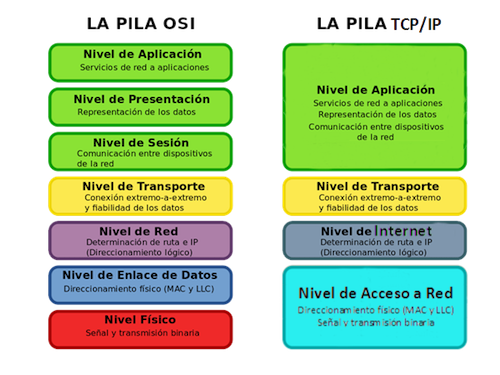
\includegraphics[scale=0.8]{imagenes/osi-tcp.png}
  \end{center}
  \caption{ Representación de capas o niveles OSI y TCP/IP.}
  \label{diagram:modelo-osi-tcp}
\end{figure}

Los sockets dentro del modelo TCP/IP se pueden ver como una interfaz con la capa de transporte.

\begin{figure}[H]
  \begin{center}
    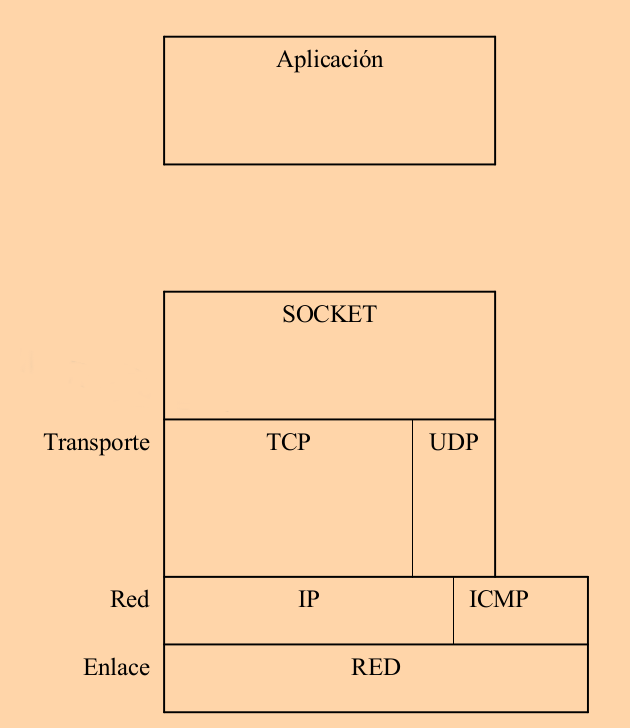
\includegraphics[scale=0.5]{imagenes/modelo-tcp-ip-socket.png}
  \end{center}
  \caption{ Representación de los sockets como una interfaz de la capa de transporte del protocolo TCP/IP.}
  \label{diagram:socket}
\end{figure}


\section{Streaming}
\label{sec:def-streaming}

La retransmisión (en inglés streaming, también denominado transmisión) es la distribución digital de contenido multimedia a través de una red de computadoras, 
de manera que el usuario utiliza el producto a la vez que se es descargado. La palabra retransmisión se refiere a una corriente continua que fluye sin interrupción, habitualmente audio o vídeo, aplicándose la difusión 
de vídeo en el presente proyecto. \\

Este tipo de tecnología funciona mediante un búfer de datos que va almacenando el flujo de descarga en la estación del usuario para inmediatamente mostrarle el material descargado. Esto se contrapone al mecanismo de
descarga de archivos, que requiere que el usuario descargue los archivos por completo para poder acceder al contenido.\\

La retransmisión requiere de una conexión por lo menos de igual ancho de banda que la tasa de transmisión del servicio. La retransmisión de vídeo por Internet se popularizó a fines de la década de 2000, 
cuando la contratación del suficiente ancho de banda para utilizar estos servicios en el hogar se hizo lo suficientemente barato.

\section{Comunicación serie}

La comunicación serie o comunicación secuencial, en telecomunicaciones e informática, es el proceso de envío de datos de un bit a la vez, de forma secuencial, sobre un canal
de comunicación o un bus.\\

En cambio, en la “comunicación en paralelo” todos los bits de cada símbolo se envían al mismo tiempo, y por ello debe haber al menos tantas líneas de comunicación como bits tenga
la información a transmitir.\\

\subsection{Características}

La ventaja de la comunicación serie es que necesita un número más pequeño de líneas de transmisión que una comunicación paralela que transmita la misma información. Esta última
necesita tantas líneas de transmisión como la cantidad de bits que componen la información, mientras que la primera se puede llevar a cabo con una sola línea de transmisión. Por otra parte,
surgen una serie de problemas en la transmisión de un gran número de bits en paralelo, como los problemas de interferencia o desincronización.\\

A la misma frecuencia de transmisión, la comunicación paralela tiene un mayor rendimiento. La comunicación serie tiene que compensar esta debilidad con una frecuencia más alta.\\

Ejemplos:\\

\begin{itemize}
 \item Código Morse
 \item Ethernet
 \item Fibre Channel
 \item FireWire
 \item I²C
 \item MIDI
 \item PCI Express
 \item RS-232
 \item RS-485
 \item Serial ATA
 \item Serial Peripheral Interface
 \item Universal Serial Bus
\end{itemize}

\section{PWM}

La modulación de ancho de pulso (PWM) o la modulación de duración de pulso (PDM) es una técnica de modulación utilizada para codificar un mensaje en una señal de pulso. 
Aunque esta técnica de modulación puede utilizarse para codificar información para la transmisión, su uso principal es permitir el control de la potencia suministrada a los
dispositivos eléctricos, especialmente a cargas inerciales tales como motores. Además, PWM es uno de los dos principales algoritmos utilizados en los cargadores de baterías solares
fotovoltaicas, el otro es el seguimiento del punto de máxima potencia.\\

El valor promedio de voltaje (y corriente) alimentado a la carga se controla al encender y apagar el interruptor entre suministro y carga a una velocidad rápida. Cuanto más tiempo
esté encendido el interruptor en comparación con los períodos de desconexión, mayor será la potencia total suministrada a la carga.\\

La frecuencia de conmutación de PWM debe ser mucho más alta que la que afectaría a la carga (el dispositivo que usa la potencia), lo que significa que la forma de onda resultante
percibida por la carga debe ser lo más suave posible. La velocidad (o frecuencia) a la que debe cambiar la fuente de alimentación puede variar mucho según la carga y la aplicación,
por ejemplo:\\

El cambio debe hacerse varias veces por minuto en una estufa eléctrica; 120 Hz en un atenuador de lámpara; entre unos pocos kilohercios (kHz) y decenas de kHz para un accionamiento
de motor; y en las decenas o cientos de kHz en amplificadores de audio y fuentes de alimentación de computadoras.\\


El término ciclo de trabajo describe la proporción de tiempo \quotes{conectado} al intervalo regular o \quotes{período} de tiempo; un ciclo de trabajo bajo corresponde a la baja potencia,
ya que la energía está apagada la mayor parte del tiempo. El ciclo de trabajo se expresa en porcentaje, 100\% siendo completamente activado.
La principal ventaja de PWM es que la pérdida de potencia en los dispositivos de conmutación es muy baja. Cuando un interruptor está apagado prácticamente no hay corriente, y 
cuando está encendido y la energía se transfiere a la carga, casi no hay caída de tensión en el interruptor. La pérdida de potencia, al ser el producto de voltaje y corriente, es,
por lo tanto, en ambos casos cercano a cero. PWM también funciona bien con controles digitales, que, debido a su naturaleza de encendido/apagado, pueden establecer fácilmente el 
ciclo de trabajo necesario.\\


% Este archivo es parte de la memoria del proyecto fin de carrera
% de Manuel López Urbina. Protegida bajo la licencia GFDL.
% Para más información, la licencia completa viene incluida en el
% fichero fdl-1.3.tex

% Copyright (C) 2018 Manuel López Urbina

\chapter[Estado del arte y herramientas utilizadas]{Estado del arte y herramientas utilizadas}
\chaptermark{Arte y tecnologías}
\label{chap:herramientas}


\section{ Estado del arte }

\subsection{Introducción}

REDACTAR ESTADO DEL ARTE

En la actualidad podemos observar cómo la robótica cada vez se encuentra más presente en nuestras vidas cotidianas tanto como para facilitarnos ciertas tareas como para entretenimiento. Si realizamos 
cualquier búsqueda en internet podemos encontrar multitud de proyectos robóticos en la red. Existen excelentes portales como \url{http://blog.bricogeek.com/} por nombrar alguno de ellos, donde se
publican multitud de proyectos novedosos y originales donde sus autores describen su desarrollo y por regla general lo acompañan de un vídeo donde se demuestra su funcionamiento.\\

Existen también comunidades que organizan competiciones de drones y/o robots, comunidades educativas asociadas a alguna tecnología concreta como pueden ser Arduino o Raspberry Pi, etcétera, donde nuevamente todas las 
descripciones de los diferentes proyectos se realizan con la documentación oportuna y en la mayoría de los casos acompañadas de un vídeo demostrativo con la inexistencia de interacción directa por parte 
del usuario.\\

Todo esto en lo referente a un contexto cotidiano en la actualidad, en la sección \ref{sec:referencias} se citan algunas de las referencias consultadas con la finalidad de contextualizar el proyecto 
en un ámbito más científico.\\

\subsection{ Referencias }
\label{sec:referencias}

Tras la realización de un sondeo entre numerosas bases de datos de artículos científicos existentes, indicar la existencia de artículos cuya temática guardan similitud con la problemática presentada
en cuanto a los requisitos y características del presente proyecto. Dichos artículos han sido tomados como punto de partida para el abordaje del problema y su estudio.\\

Existen numerosos artículos en los que se aborda el diseño y desarrollo y teleoperación de sistemas robóticos mediante la utilización de WebSockets y mediante la programación de microcontroladores. Por citar algunos de ellos como; \emph{Design and Development of a Robotic Teleoperation System using
Duplex WebSockets suitable for Variable Bandwidth Networks} \cite{article:1}, en el que se describe el desarrollo de un sistema teleoperable por WebSockets.\\
  
Otros estudios, en cambio, se centran más en analizar las diferentes situaciones de sobrecarga en la red, anchos de banda, cargas del sistema, etcétera, con la finalidad de someter a pruebas de estrés
los diferentes protocolos implicados. Como por ejemplo: \emph{Analysis of WebSockets as the New Age Protocol for Remote Robot Tele-operationt} \cite{article:2}.\\
  
Por otra parte, el artículo \emph{ Remote Monitoring System based on a Wi-Fi Controlled Car Using Raspberry Pi } \cite{article:3}, describe un sistema de monitorización construido sobre una placa 
Raspberry Pi de las mismas características que la empleada para el robot SensorRS.\\ 
  
Es, por todo lo anterior, que en el presente proyecto se ha intentado dotar al sistema de una característica añadida. Permitir el seguimiento por parte parte del usuario que realiza las funciones de teleoperador. Además de enfocarlo
desde la perspectiva del entretenimiento y la enseñanza.\\


\section{Tecnologías software utilizadas}
\sectionmark{Tecnologías software}

A continuación se detallan las diferentes tecnologías/bibliotecas/lenguajes que se han empleado para la elaboración del proyecto y por qué se han escogido por encima de otras posibles soluciones.

\subsection{\LaTeX}

Web: \url{https://www.latex-project.org/}\\

\LaTeX \: es un lenguaje de marcado que sirve para la redacción de documentos científicos o técnicos. Con esta herramienta o lenguaje se ha desarrollado la memoria actual del proyecto de final de carrera.\\

Para el estudio de la herramienta y realización de consultas se han empleado sobre los recursos bibliográficos \cite{book:LaTeX} y \cite{website:6}.\\


\subsection{WebStorm}

\hspace*{2.25in}{
\includegraphics[scale=0.25]{imagenes/webstorm-logo.png}}

Web: \url{https://www.jetbrains.com/webstorm/}\\

WebStorm es un IDE de JavaScript ligero pero potente, perfectamente equipado para el desarrollo del lado del cliente (vehículo robótico) con Node.js. Para el desarrollo de la aplicación se optó por este IDE. \\

\subsection{Fritzing}

\hspace*{2.25in}{
\includegraphics[scale=0.5]{imagenes/fritzing-logo.png}}

Web: \url{https://http://fritzing.org/home//} \cite{website:1} \\

\\Fritzing es una iniciativa de hardware de código abierto que hace que los productos electrónicos sean accesibles como material creativo para cualquier persona.\\

Permitiendo la realización de diagramas, circuitos electrónicos y montajes, también sirve para hacer circuitos impresos PCB de manera profesional.

\subsection{Arduino IDE}

\hspace*{2.25in}{
\includegraphics[scale=0.5]{imagenes/arduino-logo.png}}

Web: \url{https://http://arduino.cc//} \cite{website:1} \\

El entorno de desarrollo ofrecido por Arduino resulta extremadamente sencillo de utilizar y de gran simpleza ya que el programa se escribe en la zona del sketch. Para compilarlo y
cargarlo a cualquier placa tan solo es necesario pulsar un botón.\\


\subsection{Github}

\hspace*{2.25in}{
\includegraphics[scale=0.25]{imagenes/github-logo.png}}

Web: \url{https://about.github.com/} \cite{website:2} \\
Repositorio: \url{https://github.com/lopi87/SensorRS}\\


GitHub es una forja (plataforma de desarrollo colaborativo) para alojar proyectos utilizando el sistema de control de versiones Git. Utiliza el framework Ruby on Rails por GitHub, Inc. (anteriormente conocida como Logical Awesome). Desde enero de 2010, GitHub opera bajo el nombre de GitHub, Inc. El código se almacena de forma pública, 
aunque también se puede hacer de forma privada, creando una cuenta de pago.\\

\subsection{Git}

\hspace*{2.1in}{
\includegraphics[scale=0.5]{imagenes/git-logo.png}}

Web: \url{https://git-scm.com/}\\

Git es un sistema open-source de control de versiones diseñado para manejar íntegramente las fases de desarrollo de proyectos, simples y complejos, con velocidad y eficiencia.\\

Para su estudio y afianzado de conocimientos, ya que este sistema de control de versiones me resultaba muy familiar incluso antes de comenzar con el desarrollo del presente proyecto, se ha empleado 
la referencia bibliográfica \cite{book:git}. La cual hace un recorrido por todas las posibilidades que brinda esta herramienta.\\


\subsection{Amazon Web Services (AWS) }

\begin{center}
\includegraphics[scale=0.25]{imagenes/aws_logo.png}\end{center}

Web: \url{https://aws.amazon.com/es}\\

Amazon Web Services (AWS) es una plataforma de servicios de nube que ofrece potencia de cómputo, almacenamiento de bases de datos, entrega de contenido y otra funcionalidad para ayudar a las empresas a escalar y crecer. Explore cómo millones de clientes aprovechan los productos y soluciones de la nube de AWS para crear aplicaciones sofisticadas y cada vez más flexibles, escalables y fiables.\\

\begin{sidewaysfigure}[H]
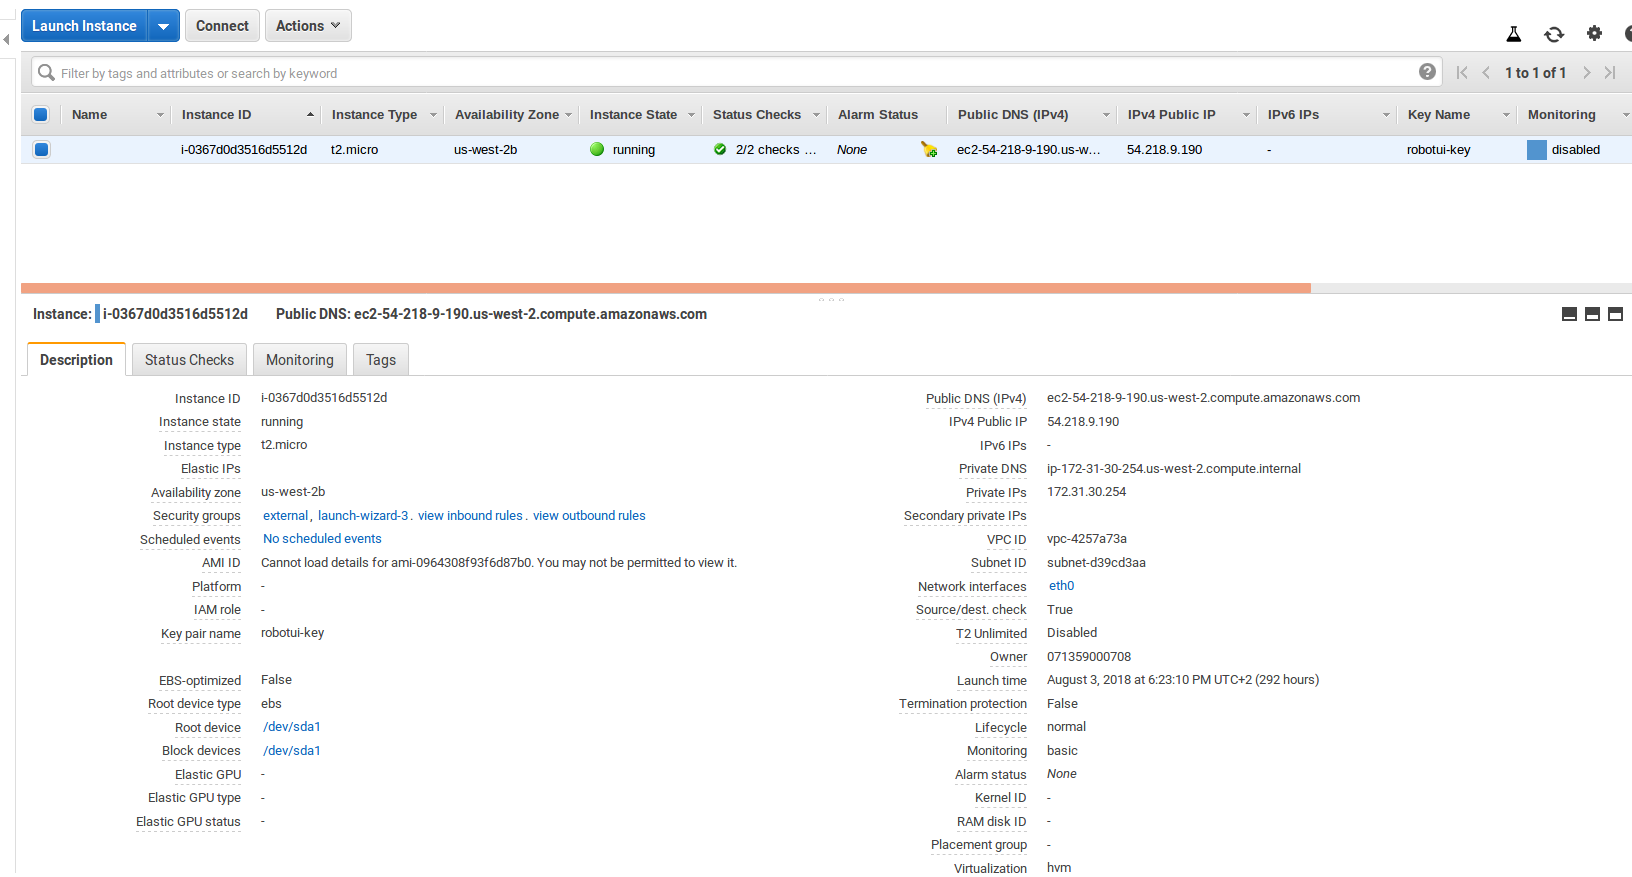
\includegraphics[scale=0.3]{imagenes/aws_instance.png}
\caption{Instancia RobotUI en AWS}
\end{sidewaysfigure}


\subsection{Node js}

\begin{center}

\includegraphics[scale=0.3]{imagenes/nodejs-logo.png}
\end{center}

Web: \url{https://nodejs.org/es/}\\
documentación: \url{https://nodejs.org/es/docs/}\cite{website:4}\\

Node.js es un entorno de ejecución para JavaScript construido con el motor de JavaScript V8 de Chrome. Node.js usa un modelo de operaciones E/S sin bloqueo y orientado a eventos, que lo hace liviano y eficiente. Incorpora un sistema de gestión de paquetes llamado, npm, es el ecosistema mas grande de librerías de código abierto en el mundo.\\

Node.js tiene una arquitectura basada en eventos capaz de E/S asíncronos. Estas opciones de diseño apuntan a optimizar el rendimiento y la escalabilidad en aplicaciones Web con muchas operaciones de entrada/salida, así como para aplicaciones Web en tiempo real (por ejemplo, programas de comunicación en tiempo real y juegos de navegador), lo que lo hacen ideal para este proyecto.\\

Destacar la importancia de la referencia bibliográfica \cite{book:javascript} para el estudio de tanto Node.js como JavaScript y que han servido de guía y consulta en la elaboración del presente proyecto. 
Sin olvidar la documentación oficial de Node.js \cite{website:4}.\\

\subsection{Npm}

\begin{center}

\includegraphics[scale=0.4]{imagenes/npm-logo.png}
\end{center}

Web: \url{https://www.npmjs.com/}\\

Npm es el gestor de paquetes por defecto para Node.js, un entorno de ejecución para JavaScript. Utilizado para la descarga de las librerías incorporadas al proyecto.


\subsection{SocketIO}

\begin{center}

\includegraphics[scale=0.3]{imagenes/socketio-logo.png}
\end{center}

Web: \url{https://socket.io/}\\

Socket.IO es una biblioteca de JavaScript para aplicaciones web en tiempo real. Permite la comunicación bidireccional en tiempo real entre clientes web y servidores. Consta de dos partes: una biblioteca del lado del cliente
que se ejecuta en el navegador y una biblioteca del lado del servidor para Node.js. Ambos componentes tienen una API casi idéntica. Al igual que Node.js, es impulsado por eventos.

Socket.IO puede usarse simplemente como un wrapper para WebSocket aunque proporciona muchas más funciones, incluyendo la transmisión a múltiples sockets, almacenamiento de datos asociados a cada cliente y E/S asíncronas.


\subsection{ FFmpeg }


\begin{center}

\includegraphics[scale=0.75]{imagenes/Ffmpeg-logo.jpg}
\end{center}

Web: \url{https://ffmpeg.org/}\\

FFmpeg es una colección bibliotecas software libre que permiten grabar, convertir (transcodificar) y hacer streaming de audio y vídeo. Incluye libavcodec, una biblioteca de códecs. FFmpeg está desarrollado en GNU/Linux, pero puede ser compilado
en la mayoría de los sistemas operativos, incluyendo Windows.\\

FFmpeg es un programa bastante sencillo y de fácil utilización, orientado tanto a personas con conocimientos avanzados como usuarios inexpertos. \\

El proyecto FFmpeg está compuesto por:\\

\begin{itemize}
 \item ffmpeg: es una herramienta de línea de comandos para convertir audio o video de un formato a otro. También puede capturar y codificar en tiempo real desde DirectShow, una tarjeta de televisión u otro dispositivo compatible.
 \item ffserver: es un servidor de streaming multimedia de emisiones en directo que soporta HTTP (la compatibilidad con RTSP está en desarrollo). Todavía no está en fase estable, y de momento no está disponible para Windows.
 \item ffplay: es un reproductor multimedia basado en SDL y las bibliotecas FFmpeg.
 \item libavcodec: es una biblioteca que contiene todos los códecs de FFmpeg. Muchos de ellos fueron desarrollados desde cero para asegurar una mayor eficiencia y un código altamente reutilizable.
 \item libavformat: es una biblioteca que contiene los multiplexadores/demultiplexadores para los archivos contenedores multimedia.
 \item libavutil: es una biblioteca de apoyo que contiene todas las rutinas comunes en las diferentes partes de FFmpeg.
 \item libpostproc: es una biblioteca de funciones de postproceso de vídeo.
 \item libswscale: es la biblioteca de escalado de vídeo.
\end{itemize}

Para el desarrollo de SensorRS, concretamente para la transmisión de vídeo desde el robot desarrollado hacia el servidor (aplicación web), el módulo utilizado ha sido el de la herramienta de línea de comandos.


\subsection{Bootstrap}


\begin{center}

\includegraphics[scale=0.3]{imagenes/bootstrap-logo.jpg}
\end{center}

Web: \url{http://getbootstrap.com/}\\

Bootstrap es un framework o conjunto de herramientas de código abierto para diseño de sitios y aplicaciones web. Contiene plantillas de diseño con tipografía, formularios, botones, cuadros, menús de navegación y otros elementos de diseño basado en HTML y CSS, así como, extensiones de JavaScript opcionales adicionales.
Se ha utilizado en el presente proyecto para la maquetación de la aplicación. En el presente proyecto se ha aprovechado para actualizarlo a la verisón 4.1.3, la más reciente hasta la fecha.\\  

\subsection{JQuery}


\begin{center}

\includegraphics[scale=0.7]{imagenes/jquery-logo.png}
\end{center}

Web: \url{https://jquery.com/}\\

JQuery es una biblioteca de JavaScript rápida, pequeña y característica. Hace que las cosas como manipulación del código HTML, manejo de eventos, animación, y permite la realización de 
peticiones Ajax de manera mucho más simple gracias a API de fácil manejo, la cual funciona a través de una multitud de navegadores. Gracias a su combinación de versatilidad y extensibilidad jQuery
ha cambiado la forma en que millones de personas desarrollan con JavaScript.\\


\section{Tecnologías hardware y materiales utilizados}
\sectionmark{Tecnologías hardware}
\label{sec:tecnologias-hardware}

A continuación se detallan las diferentes tecnologías hardware que se han
empleado para la elaboración del vehículo robótico con la finalidad de servir de prototipo durante el desarrollo de la aplicación y a modo demostrativo de la misma. En los sucesivos puntos
se describen las características de cada una de ellas junto con el motivo de su elección.


\subsection{Raspberry Pi Model B}
\label{sec:raspberry}


\begin{center}

\includegraphics[scale=0.3]{imagenes/RaspberryPi-logo.png}
\end{center}

Web: \url{https://www.raspberrypi.org}\\

Raspberry Pi es un ordenador de tamaño reducido y de bajo coste desarrollado en Reino Unido por la Fundación Raspberry Pi, con el objetivo de estimular la enseñanza de ciencias de la computación
en las escuelas. Es ampliamente utilizado y de uso muy extendido por lo que ha sido el principal motivo de su elección, además de su bajo cote y versatilidad.\\

La Raspberry Pi 3 es la tercera generación de Raspberry Pi. Sus especificaciones son las siguientes:

\begin{itemize}
 \item Una CPU ARMv8 quad-core de 64 bits de 64 bits y 1.2 GHz.
 \item LAN inalámbrica 802.11n.
 \item Bluetooth 4.1.
 \item Bluetooth baja energía (BLE).
 \item 1 GB de RAM.
 \item 4 puertos USB.
 \item 40 conexiones GPIO.
 \item Puerto HDMI.
 \item Puerto Ethernet.
 \item Conector de audio combinado de 3,5 mm y vídeo compuesto.
 \item Interfaz de la cámara (CSI).
 \item Interfaz de pantalla (DSI).
 \item Ranura para tarjeta Micro SD.
 \item VideoCore IV núcleo de gráficos 3D. 
\end{itemize}


\begin{figure}[H]
  \begin{center}
    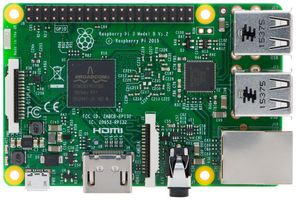
\includegraphics[scale=0.6]{imagenes/raspberry-pi.jpg}\\
    \caption{Imagen de una Raspberry Pi 3 Model B}
  \end{center}
\end{figure}


\subsection{ Arduino }

\begin{center}

\includegraphics[scale=0.6]{imagenes/arduino_logo.png}
\end{center}

Web: \url{https://www.arduino.cc/}\\

Arduino es una compañía open source y open hardware, así como un proyecto y comunidad internacional que diseña y manufactura placas de desarrollo de hardware para construir
dispositivos digitales y dispositivos interactivos que puedan sensar y controlar objetos del mundo real. Arduino se enfoca en acercar y facilitar el uso de la electrónica y 
programación de sistemas embebidos en proyectos multidisciplinarios. Los productos que vende la compañía son distribuidos como Hardware y Software Libre, bajo la Licencia Pública 
General Reducida de GNU (LGPL) o la Licencia Pública General de GNU (GPL),1​permitiendo la manufactura de las placas Arduino y distribución del software por cualquier individuo.
Las placas Arduino están disponibles comercialmente en forma de placas ensambladas o también en forma de kits hazlo tu mismo (DIY, por sus siglas en inglés de "Do It Yourself").\\

Los diseños de las placas Arduino usan diversos microcontroladores y microprocesadores. Generalmente el hardware consiste de un microcontrolador Atmel AVR, conectado bajo la 
configuración de "sistema mínimo" sobre una placa de circuito impreso a la que se le pueden conectar placas de expansión (shields) a través de la disposición de los puertos de 
entrada y salida presentes en la placa seleccionada. Las shields complementan la funcionalidad del modelo de placa empleada, agregando circuiteria, sensores y módulos de 
comunicación externos a la placa original. La mayoría de las placas Arduino pueden ser energizadas por un puerto USB o un puerto barrel Jack de 2.5mm. La mayoría de las placas 
Arduino pueden ser programadas a través del puerto Serial que incorporan haciendo uso del Bootloader que traen programado por defecto. El software de Arduino consiste de dos 
elementos: un entorno de desarrollo (IDE) (basado en el entorno de processing y en la estructura del lenguaje de programación Wiring), y en el cargador de arranque (bootloader,
por su traducción al inglés) que es ejecutado de forma automática dentro del microcontrolador en cuanto este se enciende. Las placas Arduino se programan mediante un computador, 
usando comunicación serial.\\


\begin{figure}[H]
  \begin{center}
    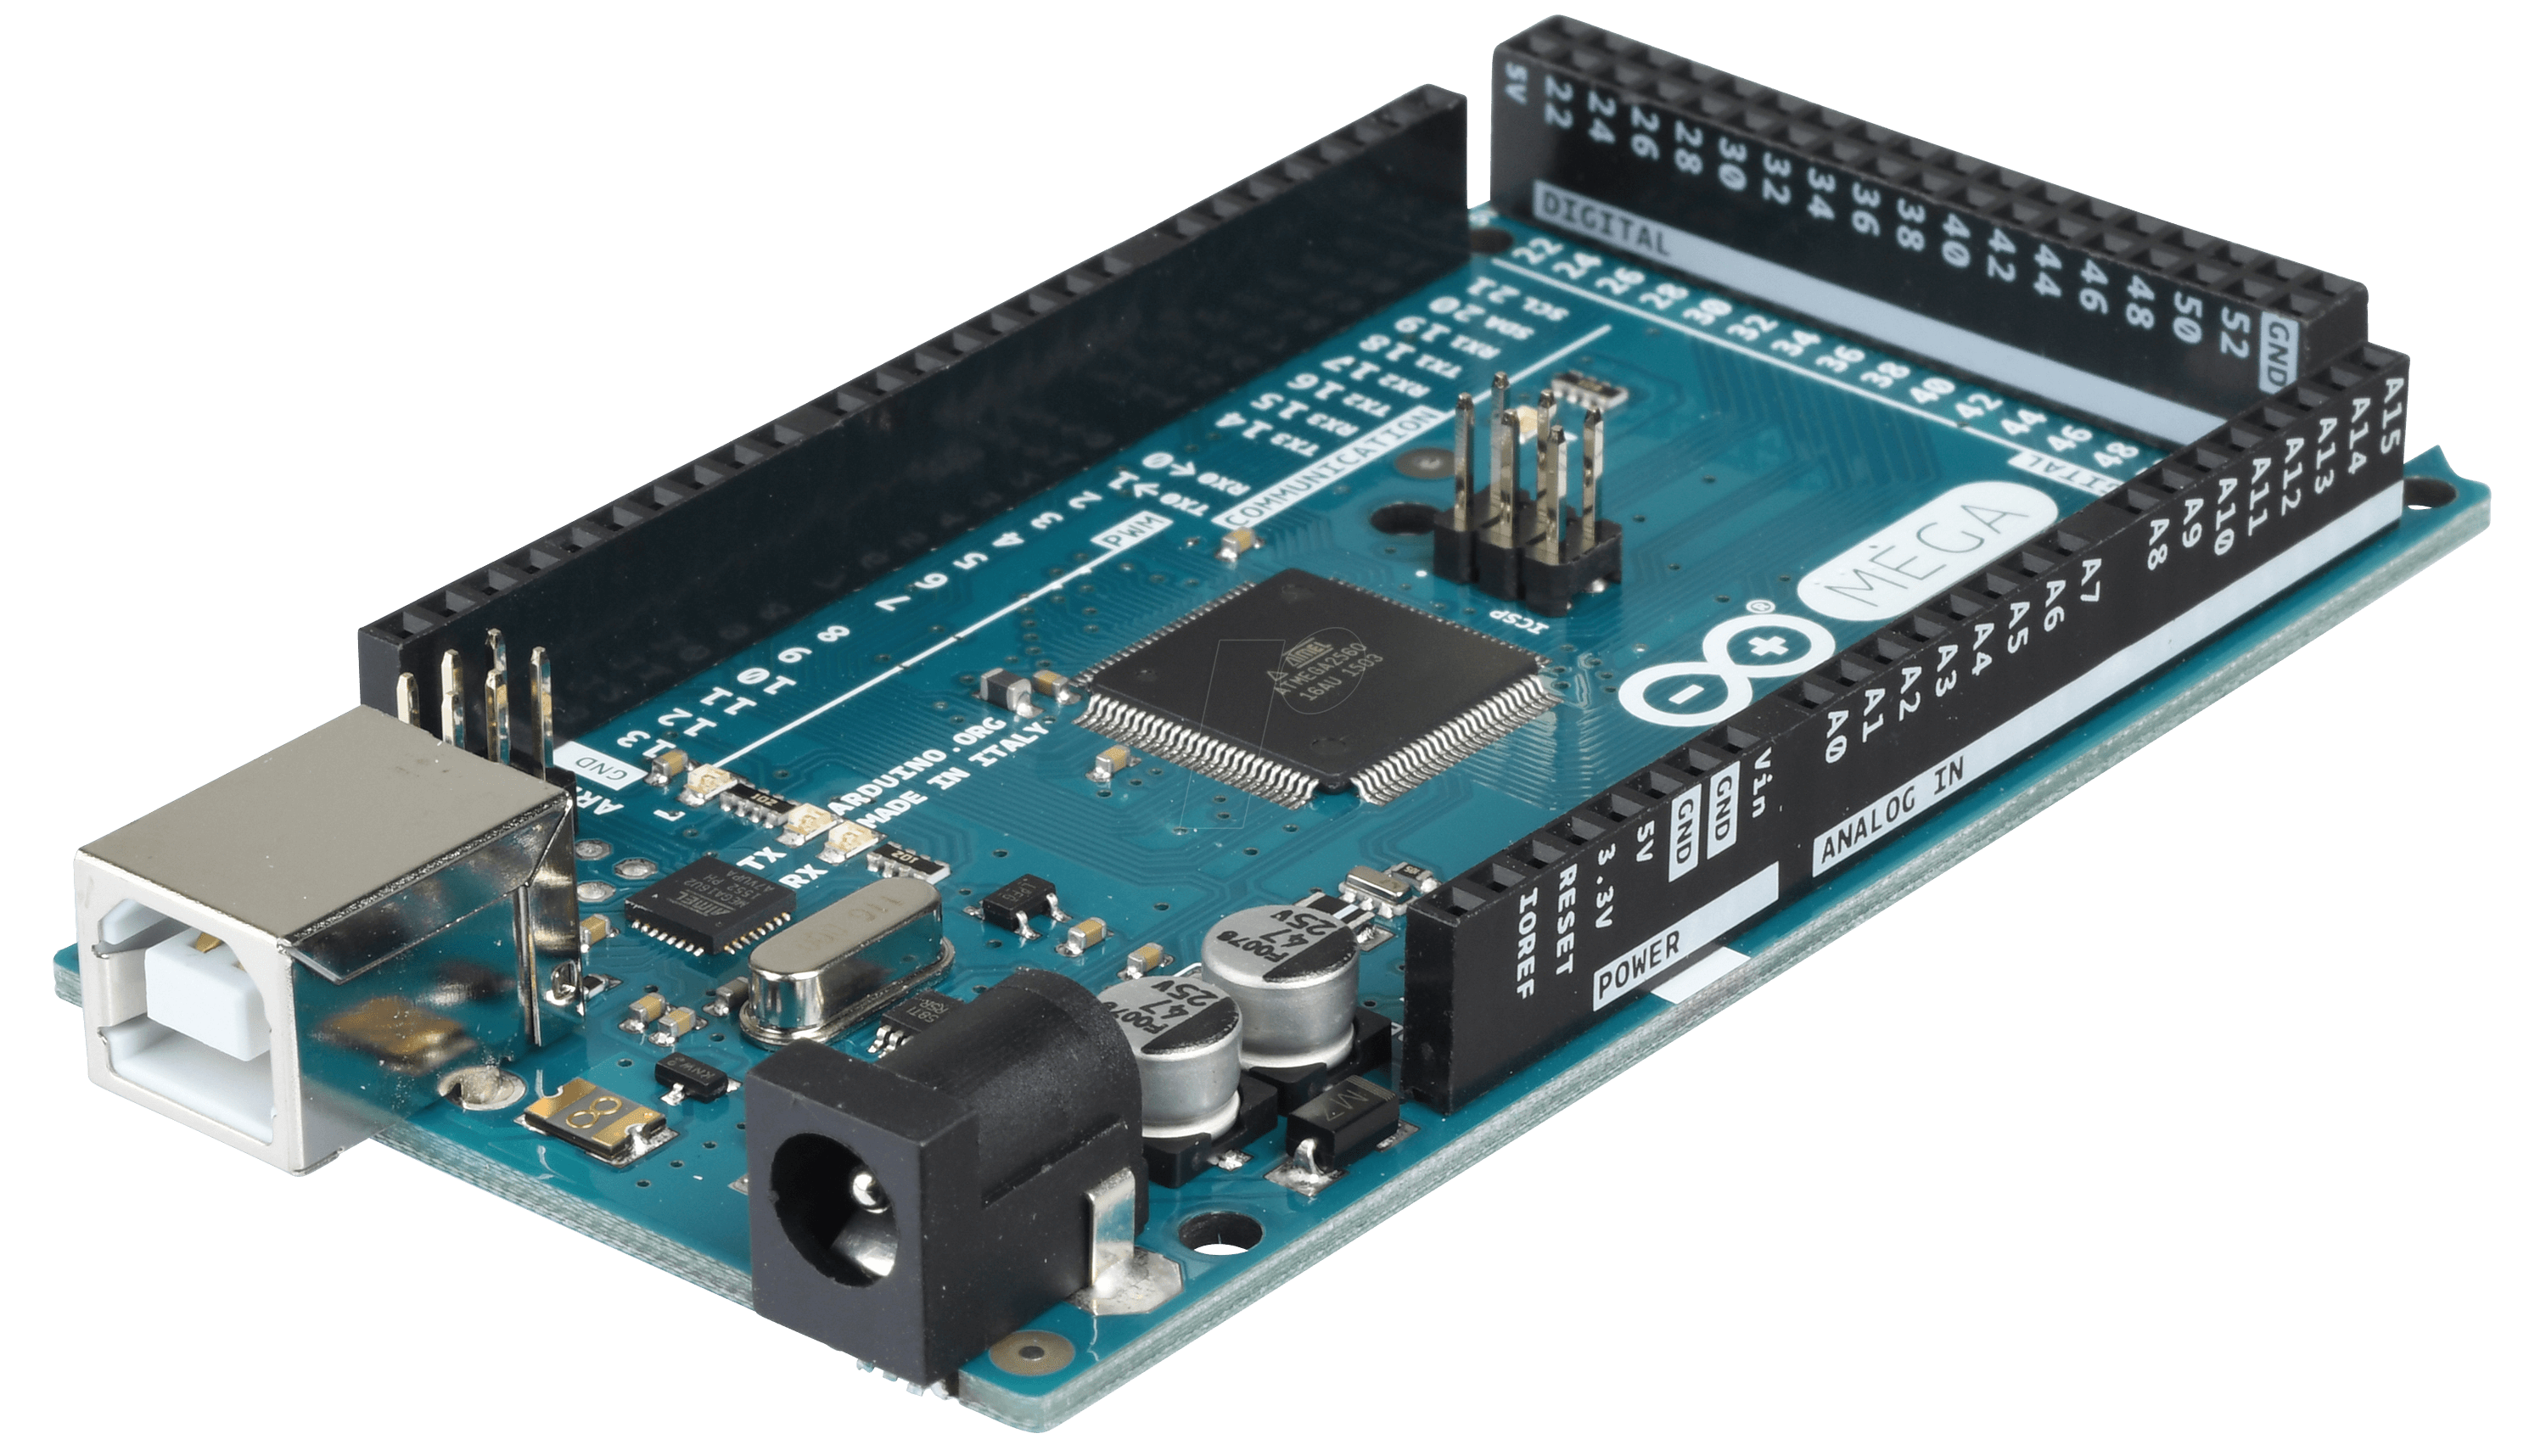
\includegraphics[scale=0.07]{imagenes/arduino_mega.png}\\
    \caption{Placa Arduino MEGA 2560}
  \end{center}
\end{figure}


Para el presente proyecto se ha utilizado la placa Arduino Mega, la cual es una tarjeta de desarrollo open-source construida con un microcontrolador modelo Atmega2560 que posee 
pines de entradas y salidas (E/S), analógicas y digitales. Esta tarjeta es programada en un entorno de desarrollo que implementa el lenguaje Processing/Wiring. Arduino puede
utilizarse en el desarrollo de objetos interactivos autónomos o puede comunicarse a un PC a través del puerto serial (conversión con USB) utilizando lenguajes como Flash,
Processing, MaxMSP, etc. Las posibilidades de realizar desarrollos basados en Arduino tienen como límite la imaginación.\\

El Arduino Mega tiene 54 pines de entradas/salidas digitales (14 de las cuales pueden ser utilizadas como salidas PWM), 16 entradas análogas, 4 UARTs (puertos serial por
hardware), cristal oscilador de 16MHz, conexión USB, jack de alimentación, conector ICSP y botón de reset.  Arduino Mega incorpora todo lo necesario para que el microcontrolador
trabaje; simplemente conéctalo a tu PC por medio de un cable USB o con una fuente de alimentación externa (9 hasta 12VDC). El Arduino Mega es compatible con la mayoría de los 
shields diseñados para Arduino Duemilanove, diecimila o UNO.

\begin{figure}[H]
  \begin{center}
    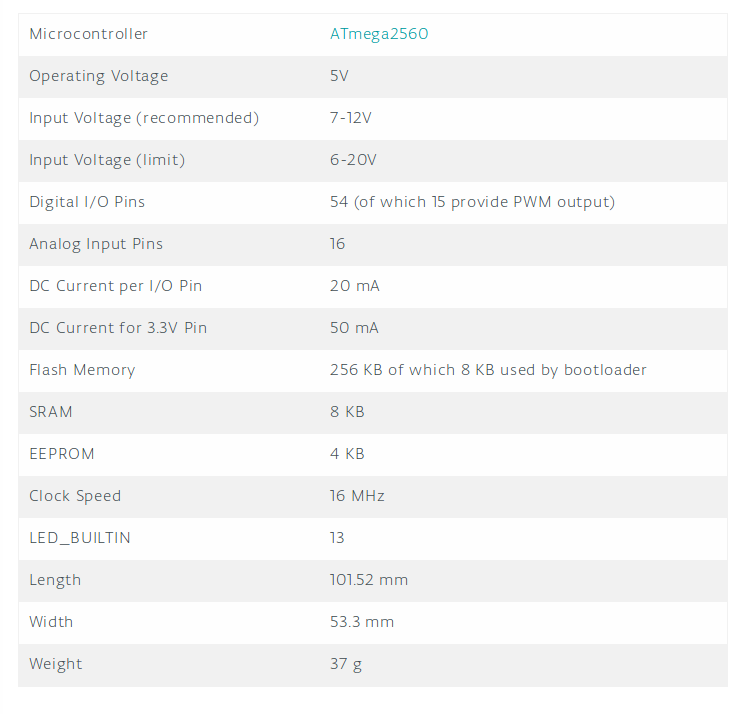
\includegraphics[scale=0.5]{imagenes/arduino_caracteristicas.png}\\
    \caption{Características Arduino MEGA 2560}
  \end{center}
\end{figure}


\subsection {Arduino sensor kit}

Se ha utilizado un pack de diversos sensores para arduino, los sensores utilizados quedarán descritos a mayor detalle en el capítulo referente a sensores \ref{chap:sensores}.

\begin{figure}[H]
  \begin{center}
    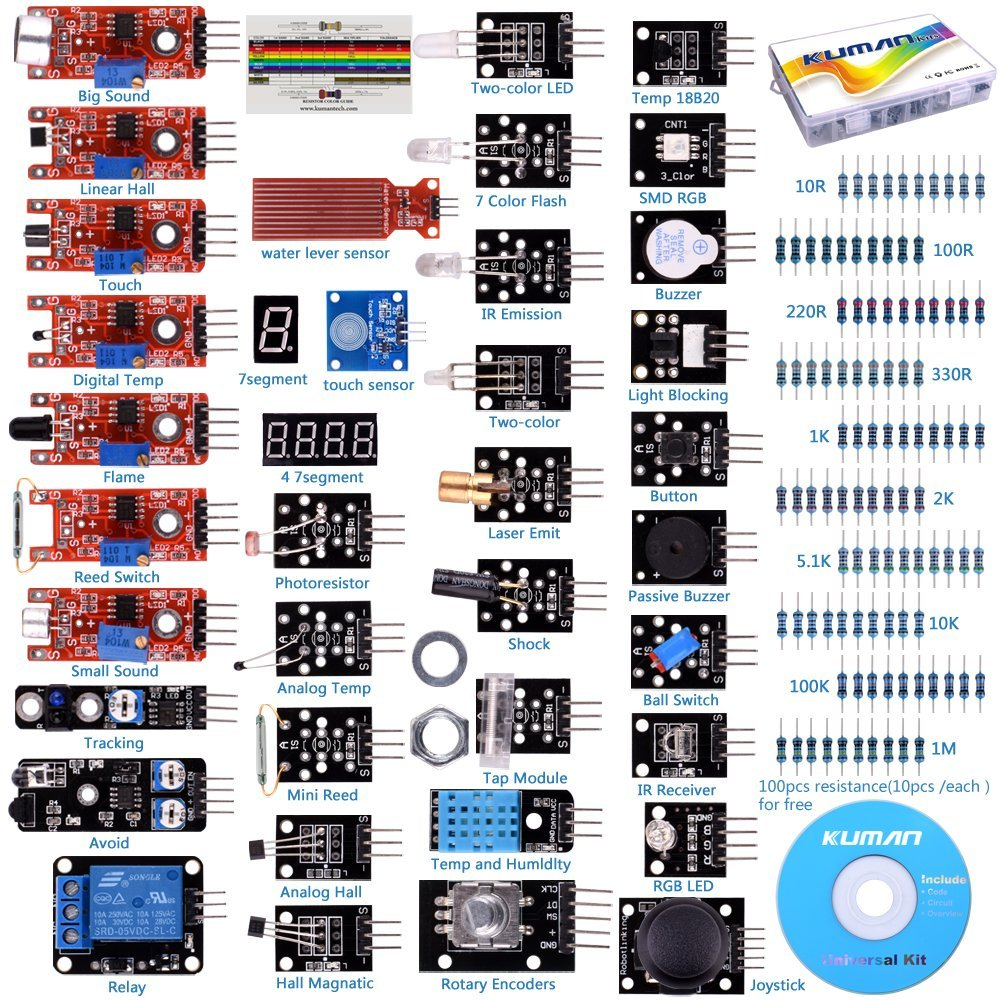
\includegraphics[scale=0.35]{imagenes/arduino_sensor_kit.jpg}\\
    \caption{Pack de sensores para Arduino}
  \end{center}
\end{figure}

\subsection{Controlador de motores doble puente H - L298N}


El módulo controlador de motores L298N H-bridge o puentes H, nos permite controlar la velocidad y la dirección de dos motores de corriente continua o un motor paso a paso de una forma muy sencilla,
gracias a los 2 los dos H-bridge que dispone.\\

Básicamente un puente-H o H-bridge es un componente formado por 4 transistores que nos permite invertir el sentido de la corriente, y de esta forma podemos 
invertir el sentido de giro del motor \footnote{Podrá acceder a información más detallada de la presente controladora en la sección correspondente al capítulo }.\\

El rango de tensiones en el que trabaja este módulo va desde 3V hasta 35V, y una intensidad de hasta 2A. A la hora de alimentarlo hay que tener en cuenta que la 
electrónica del módulo consume unos 3V, así que los motores reciben 3V menos que la tensión con la que alimentemos el módulo.\\

Además el L298N incluye un regulador de tensión que nos permite obtener del módulo una tensión de 5V, perfecta para alimentar nuestro Arduino. Eso sí, este regulador sólo 
funciona si alimentamos el módulo con una tensión máxima de 12V.\\

Es un módulo que se utiliza mucho en proyectos de robótica, por su facilidad de uso y su reducido precio, lo cual ha servido para que sea seleccionado para el presente proyecto.

\begin{figure}[H]
  \begin{center}
    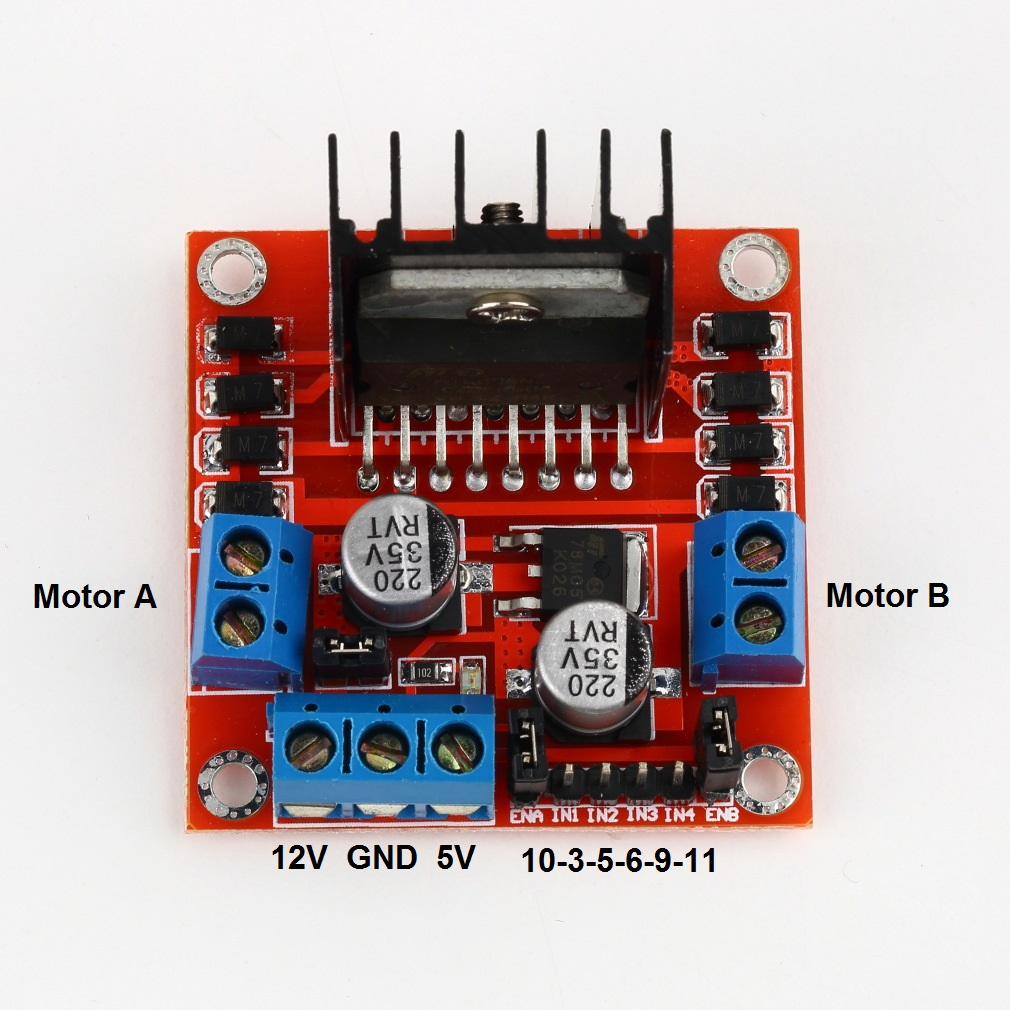
\includegraphics[scale=0.8]{imagenes/l298n.jpg}\\
    \caption{Imagen de la Controlador de motores doble puente H - L298N utilizada.}
  \end{center}
\end{figure}



\subsection{ Batería LiPo }

Para alimentar los motores y su controladora se ha empleado una batería LiPo de 1000mAh a 3,7V. Las batería de polímero de iones de litio, son pilas recargables (células de secundaria), compuestas generalmente de varias células secundarias idénticas en paralelo para aumentar la capacidad 
de la corriente de descarga. Siendo ideales para este tipo de usos.

\begin{figure}[H]
  \begin{center}
    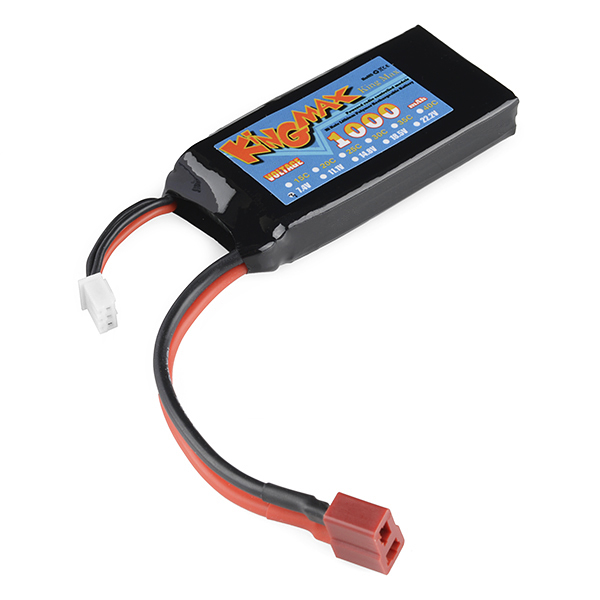
\includegraphics[scale=0.3]{imagenes/robot/bateria-lipo.jpg}\\
    \caption{Imagen de la batería LiPo utilizada.}
  \end{center}
\end{figure}


\subsection{ Tarjeta de expansión con batería de Litio para Raspberry Pi }
\label{componente:bateria-expansion}

Para la alimentación de la placa se ha optado por un módulo de potencia diseñado especialmente para la Raspberry Pi 3 Model B, permitiendo que la placa maestra trabaje sin conexión hasta 9 horas
de forma ininterrumpida.\\

Por otra parte, esta placa dispone de 2 puertos USB adicionales: uno suministra energía para la Raspberry Pi y el otro para una posible pantalla LCD, resultando interesante para otros proyectos.\\

Sus características principales son las siguientes:

\begin{enumerate}
 \item Capacidad de la batería: 3800mAH.
 \item Corriente de descarga máxima: 1.8A.
 \item Tensión de salida sin carga: 5.1V ± 0.1V.
 \item Corriente / voltaje de carga estándar: 1.0A / 5.0V.
 \item Tensión de corte de la carga completa de la batería de iones de litio: 4.18V - 4.2V.
\end{enumerate}


\begin{figure}[H]
  \begin{center}
    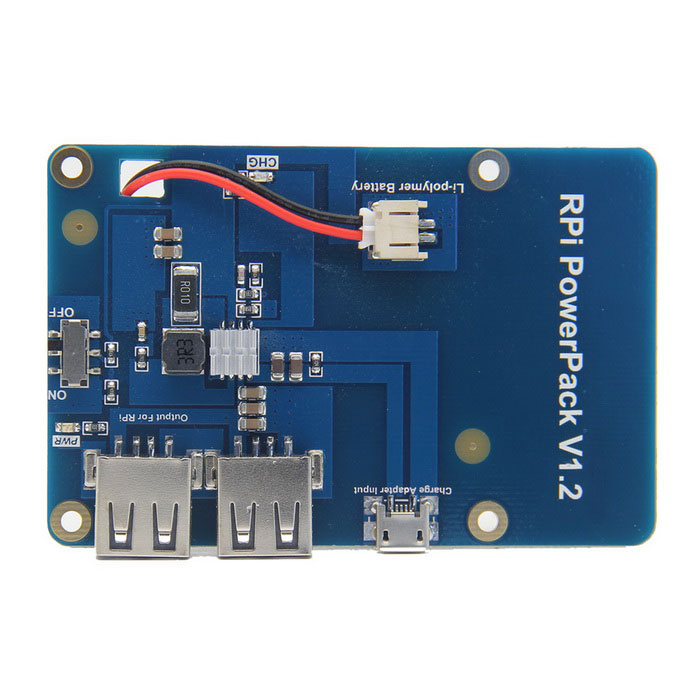
\includegraphics[scale=0.3]{imagenes/robot/modulo-alimentacion.jpg}\\
    \caption{Imagen de la tarjeta de expansión con batería de Litio utilizado.}
  \end{center}
\end{figure}

\subsection{ Cámara USB de alta definición }

Cámara USB para su conexión en la Raspberry para la emisión de imágenes. La cámara seleccionada dispone de las siguientes características:

\begin{itemize}
\item 2 megapíxeles de resolución.
\item Ángulo de visión de 170 grados.
\item Interfaz USB 2.0 de alta velocidad, refresco de 60 fps en resolución 1280X720, 30 fps en resolución 1920X1080.
\item Tamaño reducido y perfil delgado ideal para aplicaciones embebidas.
\end{itemize}

\begin{figure}[H]
  \begin{center}
    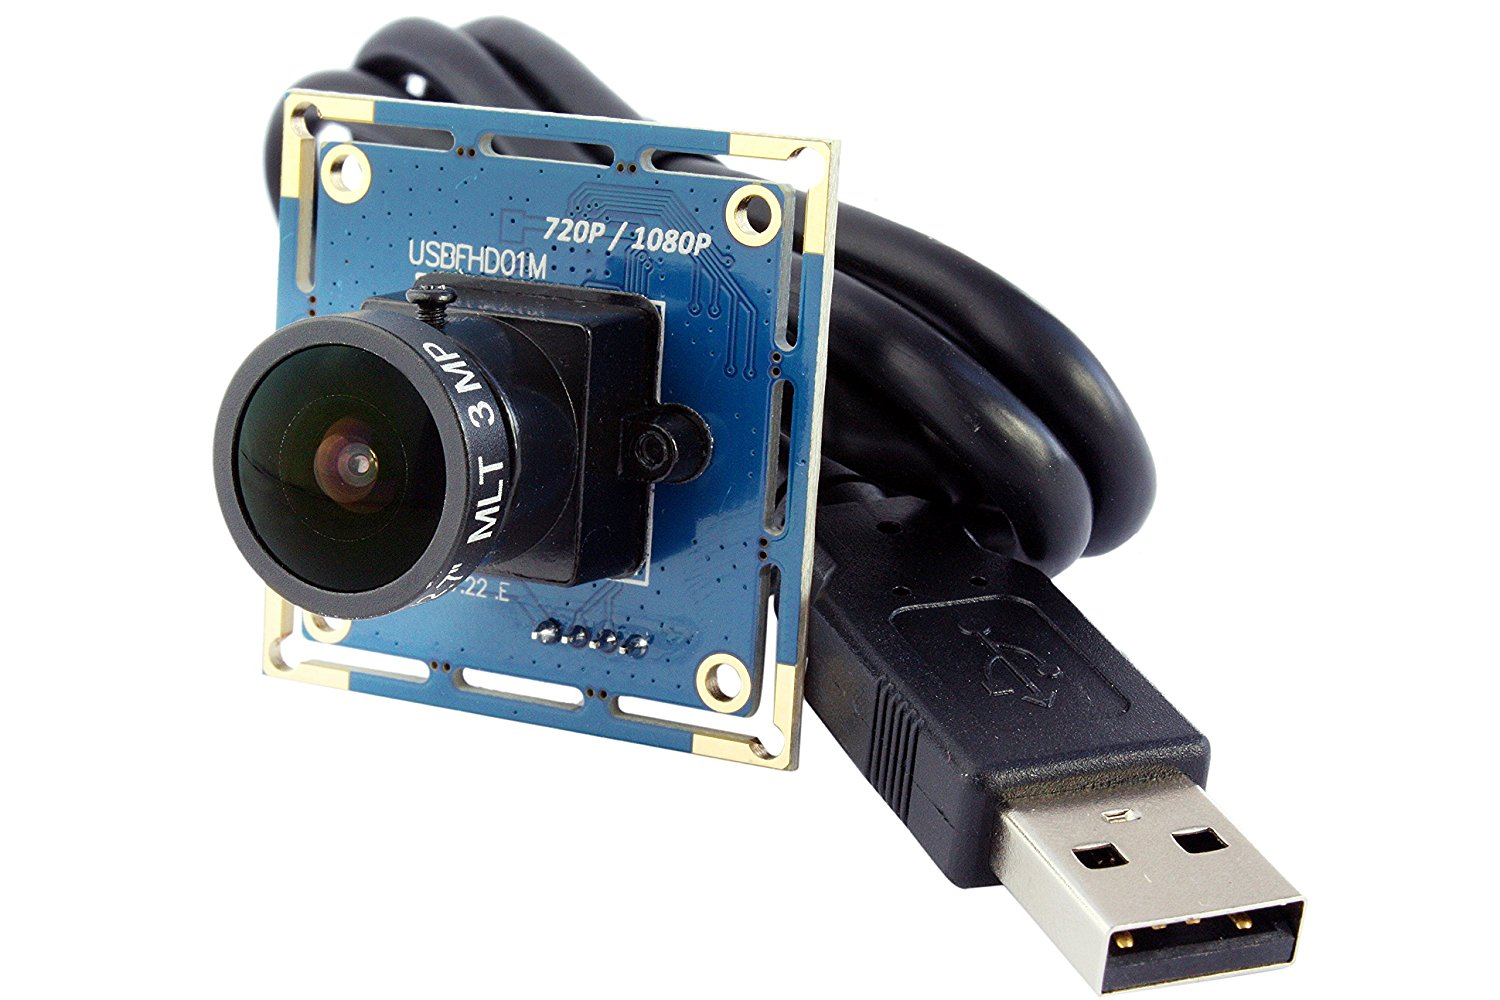
\includegraphics[scale=0.15]{imagenes/robot/camara-usb.jpg}\\
    \caption{Imagen de la cámara USB utilizada.}
  \end{center}
\end{figure}

Los motivos de su elección ha sido principalmente su facilidad de puesta en funcionamiento ya que al tratarse de una cámara USB. Tan sólo debemos conectarla para comenzar con su funcionamiento ya que es detectada 
por prácticamente todas las distribuciones Linux.\\

\subsection{Gamepad}

Gamepad inalámbrico con conexión bluethoot para el manejo del vehículo desde un dispositivo móvil gracias al sistema de acoplamiento del que dispone, Ver figura \ref{figura:control_pad}.

\begin{figure}[H]
  \begin{center}
    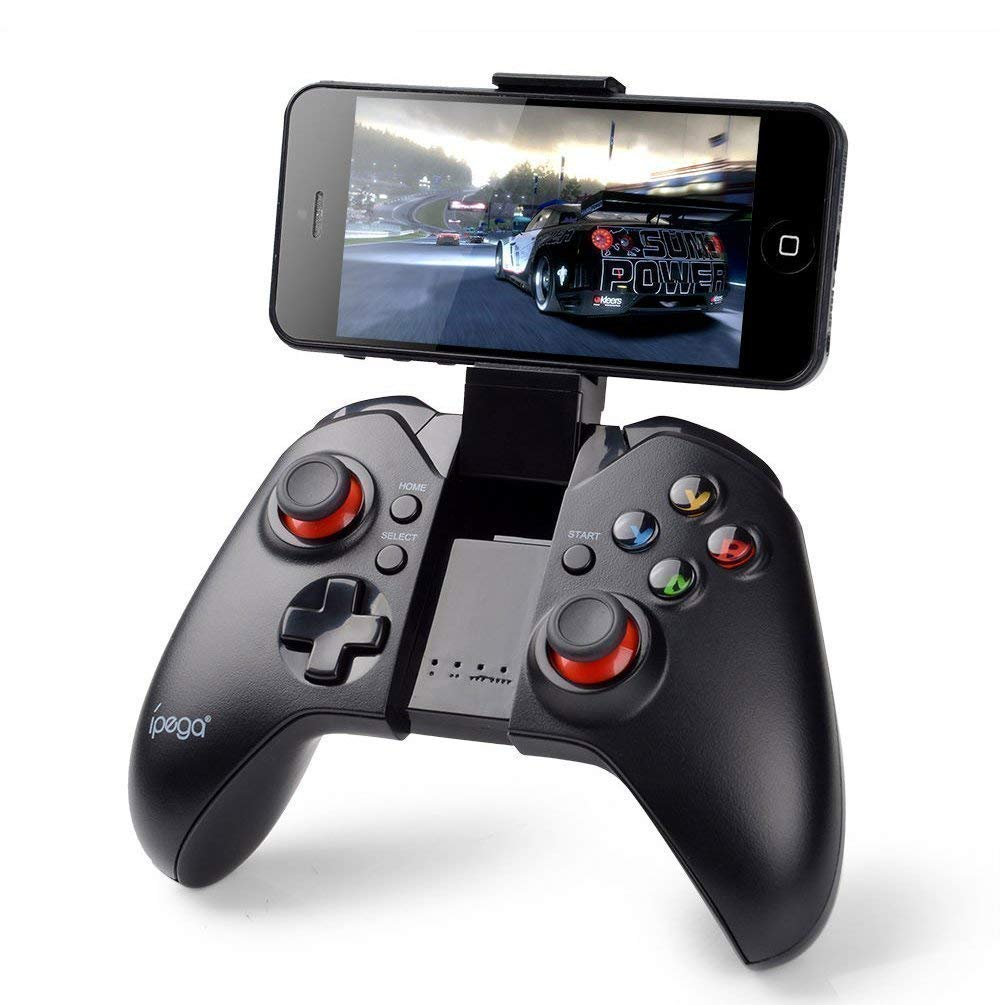
\includegraphics[scale=0.2]{imagenes/robot/control_pad.jpg}
  \end{center}
  \caption{Vista del gamepad utilizado.}
  \label{figura:control_pad}
\end{figure}

% Este archivo es parte de la memoria del proyecto fin de carrera
% de Manuel López Urbina. Protegida bajo la licencia GFDL.
% Para más información, la licencia completa viene incluida en el
% fichero fdl-1.3.tex

% Copyright (C) 2018 Manuel López Urbina

\newpage

\chapter[Requisitos]{Especificación y análisis de requisitos}
\label{chap:requisitos}

En el presente capítulo se recopilan las diferentes carcaterísticas base de obligado cumplimiento por el producto final a desarrollar. Siendo estas características definidas en una
etapa incial del presente proyecto. \\

Debido a que el proyecto implica un desarrollo tanto a nivel software como hardware se realizó una recopilación de requisitos abarcando ambas áreas por separado.\\

\section{Requerimientos hardware}
\label{sec:requerimientos-hardware}

Se ha optado por la construcción de un robot móvil dotado de un chasis de 4 ruedas donde las dos ruedas traseras serán accionadas por un motor mientras que las dos ruedas delanteras
harán de directrices.\\

El motor porpulsor funcionará a corriente continua de manera que en función de la polarización de los terminales haga girar las ruedas en una dirección o la contraria (marcha adelante o atrás), mientras que 
la dirección será accionada por un servomotor.\\

El chasis utilizado deberá permitir añadir multitud de componentes necesarios para construir el robot, deberá disponer de paneles para instalar las diferentes
placas electrónicas y sensores además de ser lo suficientemente liguero para que el sistema en su conjunto tenga agilidad en sus movimientos a la vez que resistencia.\\

El robot además deberá poder obtener imágenes de vídeo y transmitirlas al servidor donde se encuentre alojada la aplicación de control. Por lo que resulta necesario incorporar una cámara de 
pequeñas dimensiones de alta definición.\\

Por otra parte, todo robot necesita de una unidad de central de procesamiento donde se localizará el programa de control. Este programa tendrá la función de interpretar las diferentes señales recibidas,
control de sensores y dispositivos conectados. Además, esta placa es la encargada de distribuir la alimentación por los diferentes componentes hardware que lo necesiten y recibir las señales de
los sensores y enviarla a los motores.\\

Necesidad de poder acoplar multitud de sensores para medicíon de parámetros ambientales resultando necesario incorporar alguna placa dotada de un microcontrolador de fácil programación como podría ser
algunas de las placas proporcionadas por Arduino.\\

Tanto la placa que incorpore el microcontrolador y sus sensores como la unidad central de procesamiento deben disponer de un canal de comunicación para el intercambio de datos entre las mismas.\\


\subsection{Análisis y selección de componentes electŕonicos}

La informática, en los últimos años ha dado un gran impulso con proyectos como el de la Raspberry Pi Foundation, en este caso concreto en áreas como la del IOT \footnote{
Internet de las cosas (en inglés, Internet of Things, abreviado IoT o​ IdC, por sus siglas en español​) es un concepto que se refiere a la interconexión digital de objetos cotidianos
con Internet.​}. En lo referente al hardware, nunca ha sido más fácil coger componentes, juntarlos y con una mínima programación hacer algo totalmente nuevo, interesante y útil al
mismo tiempo gracias a la existencia de proyectos como Arduino.\\

En este caso, nos planteamos la siguiente incógnita; ¿Empleamos una Raspberry Pi o un Arduino?. En internet encontramos tantos y tantos proyectos por 
hacer en los que muchas veces es difícil decidirse.\\

Arduino se compone de una parte Hardware y Software. Es por ello que gracias a los emuladores existentes y sin tocar una sola pieza hardware, podemos simular un proyecto desde 
nuestro ordenador. Podemos programarlo y hacer las conexiones virtuales para ver cómo se comportaría. Arduino es una plataforma simple y dedicada precisamente a eso, 
a montar sobre ella los componentes necesarios para los proyectos. \\

La Raspberry Pi Foundation en cambio, ha diseñado y elaborado un ordenador para enseñar informática a la antigua usanza. La Raspberry Pi es un ordenador asequible, 
suficientemente potente para facilitar el aprendizaje y realizar tareas básicas. Incluso programar y compilar programas que se ejecuten en la Raspberry Pi. Y todo ello en un
tamaño mínimo, similar al de una tarjeta de crédito, alimentado con un cargador de móvil de 2 amperios y que da muchísimo juego para todo tipo de proyectos.\\

Por tanto, en respuesta a la pregunta inicial, se ha decidido que la mejor placa la elaboración del proyecto es aprovechar lo mejor de cada una de ellas. Utilizaremos tanto una Raspberry Pi
como una Arduino Mega aprovechando al máximo el potencial que ofrece cada una de ellas, cada una con sus virtudes y sus defectos.\\


\subsubsection{Ventajas y desventajas de Raspberry Pi y de Arduino}

El punto fuerte de Arduino no es su potencia de cálculo, ni la memoria de la placa, ni la frecuencia del procesador. Entonces, ¿Por qué debemos considerar dichas placas para
utilizarlas en nuestros proyectos? El punto fuerte de Arduino está en la facilidad de conectarse con el mundo, gracias a las entradas tanto analógicas como digitales con las que
cuenta y de lo fácil que resulta activar o desactivar una de las entradas/salidas gracias a su software.

Un Arduino Mega dispone 54 pines de entrada salida digital, de los cuales quince pueden ser utilizados como salidas PWM y controlar con ellos la velocidad de motores, por 
citar alguno de los ejemplos. También tiene 16 entradas analógicas, una frecuencia de 16 MHz y un conector USB y un ICSP y 4 UART. Existen muchísimos tipos de
placas Arduino y cada una con sus características específicas.\\

Otro punto a su favor es la facilidad de prototipado que ofrece y, por supuesto, los Shields o mochilas de expansión, que ofrecen dotar a nuestra placa desde conectividad Wi-Fi, 
GPS, conectividad por radio de largo alcance, displays táctiles, etc. Y muchas de ellas con un bajo coste.\\

Por el contrario la Raspberry Pi puede presumir de músculo y de potencia de cálculo comparada con las placas Arduino como memoria y capacidades multimedia, que van desde la 
reproducción de video en HD, pasando por una salida de audio (de no demasiada calidad, todo hay que decirlo, aunque hay alternativas), así como una salida de vídeo compuesto.
Y, pese a no contar con las capacidades de interconexión de Arduino y con todos sus shields, sí que contamos con (cada vez más) placas de expansión en forma de shields. 
Todo ello gracias a los conectores GPIO, I2S, etc. que incorpora la Raspberry Pi.\\

\begin{figure}[H]
  \begin{center}
    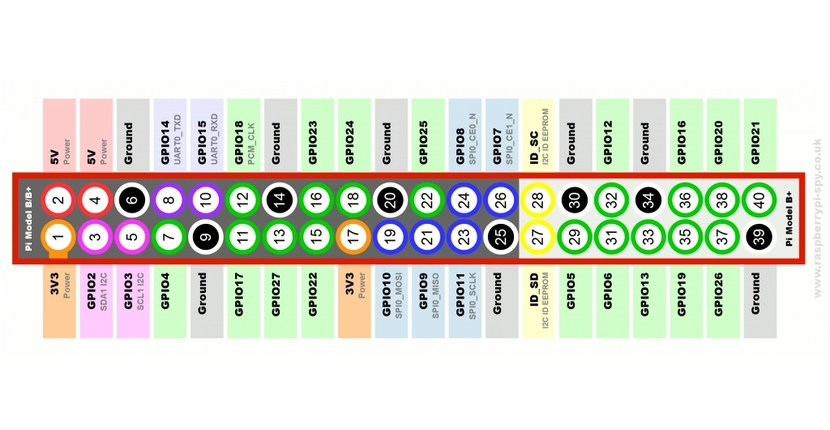
\includegraphics[scale=0.4]{imagenes/robot/gpio-conexiones.jpg}
  \end{center}
  \caption{Esquema GPIO de una Raspberry Pi Model B+.}
  \label{gantt:tareas01}
\end{figure}

Por otra parte, otro de los puntos a tener muy en cuenta es la posibilidad de incorporar las diferentes cámaras desarrolladas de diversas características y tipos diferentes como
la captación de imágenes por infrarrojos, nos damos cuenta de que la Raspberry Pi puede sustituir a un ordenador en tareas simples. Y además podemos usar sus puertos de conexión
para interconectar nuestro proyecto con el mundo como lo haríamos con un Arduino.\\

\begin{figure}[H]
  \begin{center}
    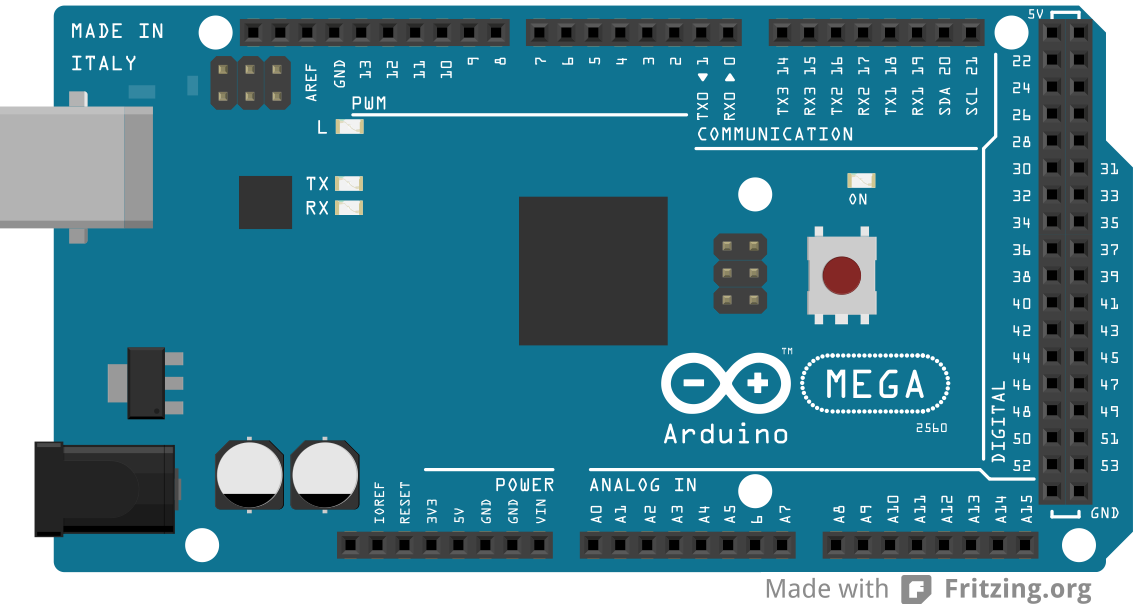
\includegraphics[scale=0.4]{imagenes/arduino_mega_pinout.png}
  \end{center}
  \caption{Placa Arduino Mega donde se visualiza la disposición de sus pines E/S.}
  \label{gantt:tareas01}
\end{figure}

Por tanto, de todo lo anterior podemos concluir Arduino y Raspberry Pi son herramientas complementarias y perfectamente utilizables para cumplir con los requisitos del presente proyecto.\\\\


\section{Requerimientos software}
\label{sec:requerimientos-software}

Habiendo detallado los requerimientos hardware para la construcción del robot pasamos al análisis de los diferentes requerimientos software para la correcta
gestión de los diferentes elementos hardware utilizados y para su correcto funcionamiento.\\

En cuanto a la programación del robot, uno de los requisitos fundamentales es el de disponer de una vía de comunicación bidireccional junto con la posibilidad de
configurar una interfaz de control personalizada en función de los sensores que se deseen utilizar y según las características del medio al que queramos adaptar nuestro vehículo.\\

Otro requerimiento software es el de la posibilidad de integrar la lectura de valores obtenidos por sensores mostrando al usuario los parámetros obtenidos y envío de órdenes
desde un servidor externo. Además de captación y transmisión de vídeo en tiempo real.\\

Todas estas especificaciones quedan resueltas mediante la utilización de la aplicación web RobotUI, la cual se ha decidido utilizar como parte software del presente proyecto.\\

Para el caso que nos concierne en el proyecto, dentro del marco de investigación que define la totalidad de la infraestructura, la funcionalidad principal del mismo a nivel 
software será:\\

\begin{itemize}
\item Definir los pasos para dar de alta un dispositivo robótico en el sistema.
\item Una vez configurado el dispositivo, configurar la interfaz de control con las acciones de control específicas.
\item Realizar un sistema de monitorización y visualización para los usuarios espectadores en tiempo real.
\item Sistema de gestión de base de datos en donde se encuentren los datos de la aplicación recogidos.
\item Panel de administración donde visualizar la información de los usuarios conectados y dispositivos en uso en tiempo real.
\end{itemize}

\section[Especificación]{Especificación de los requisitos}

En esta etapa del modelado de requisitos se captura el propósito general del sistema:

\begin{itemize}
\item Se analiza qué debe hacer el sistema.
\item Se obtiene una versión contextualizada del sistema.
\item Identifica y delimita el sistema.
\item Se determinan las características, cualidades y restricciones que debe satisfacer el sistema.
\end{itemize}

\subsection{Requisitos funcionales}

Los requisitos funcionales que se han obtenido en el sistema son los siguientes:

\begin{itemize}
\item Ser una herramienta multiplataforma y que permita a cualquier usuario definir sus propias interfaces para el control de robots.
\item Dotar de funcionalidad gráfica que permita en tiempo real con mecanismos visuales (en web) visualizar el control de dispositivos robóticos por parte de otros usuarios, modo espectador de la aplicación.
\item Proporcionar un sistema de streaming de vídeo para la difusión de imágenes a los usuarios espectadores procedentes de los robots dispongan de cámara.
\item Implementar un panel de administración para la visualización de usuarios y dispositivos conectados en tiempo real.
\end{itemize}

\subsection{Requisitos no funcionales}

Los requisitos no funcionales son aquellos que describen cualidades o restricciones del sistema que no se relacionan de forma directa con el comportamiento funcional del mismo. A continuación se especifican los más importantes del sistema:
\begin{itemize}
\item No requiere un conocimiento específico del sistema una vez puesto en funcionamiento.
\item La aplicación tendrá manual de uso.
\item La base de datos estará implementada en un lenguaje objeto no relacional como MongoDB.
\item La aplicación estará realizada en el lenguaje de programación Python.
\item La interfaz debe reflejar claramente la distinción entre las distintas partes del sistema.
\item El sistema se desplegará sobre una versión GNU Linux Debian 8 Jessie.
\item El código fuente de la aplicación seguirá un estilo uniforme y normalizado para todos los módulos del mismo.
\end{itemize}


% Este archivo es parte de la memoria del proyecto fin de carrera
% de Manuel López Urbina. Protegida bajo la licencia GFDL.
% Para más información, la licencia completa viene incluida en el
% fichero fdl-1.3.tex

% Copyright (C) 2018 Manuel López Urbina

\newpage

\chapter{Construcción del robot}
\chaptermark{Construcción del robot}
\label{chap:montaje}


En el presente capítulo se recogen todos los procedimientos para la construcción del vehículo robótico, desde el montaje a la interconexión de cada unos de sus elementos.\\

\section{Montaje}

En esta sección se recogen todas las descripciones y procedimientos seguidos y que han resultado de mayor interés a la hora de la construcción del robot y 
sus diferentes interconexiones.\\

\subsection{Chasis}

El chasis consiste en una estructura interna que sostiene, aporta rigidez y da forma a un vehículo. Es análogo al esqueleto de un animal.
Para el caso que nos compete, el vehículo desarrollado consta de un armazón​ que sirve de sujeción de los componentes mecánicos, como el sistema de propulsión y suspensión de las
ruedas, incluyendo la carrocería además de los diferentes componentes electrónicos.​ Este robot debe ser capaz de acceder a y desenvolverse por zonas de difícil acceso, por ello de
que debe disponer de un tamaño compacto que facilite el desplazamiento, lo mantenga en equilibrio en todo momento y que le permita cambiar de dirección fácilmente.\\

\subsection{Tracción y dirección}

Para generar el movimiento, se necesita algún dispositivo que proporcione una fuerza motriz encargada de desplazar el chasis y dotar de la capacidad de movimiento al robot.
Se ha optado por la incorporación de ruedas para desplazarse, debido a su mayor agilidad y fácil manejo.\\

Estos equipos suelen utilizar baterías para alimentar los motores y electrónica, y por tanto, la fuente de alimentación suele ser corriente continua. Utilizando este tipo de
fuente de alimentación, el tipo de dispositivo a utilizar suele variar respecto de las necesidades de cada equipo, en la sección \ref{sub:alimentación} se encuentra información
referente a las mismas.\\

\subsubsection{Motores de corriente continua}

El motor de corriente continua es un dispositivo eléctrico que transforma la energía eléctrica en energía mecánica, de manera que genera un movimiento rotatorio gracias a la  
acción producida por el campo magnético. Este tipo de motores son también denominados como motores de corriente directa, motor CC o motor DC.\\

En caso de nuestro vehículo dispondrá de un motor para proporcionar movimiento a las ruedas traseras y otro de menor potencia para dotar de movimiento lateral a las delanteras 
a modo de dirección.\\

\subsubsection{Servomotores}

Los servomotores son dispositivos capaces de llevar el motor a posiciones angulares específicas al enviar una señal codificada manteniendo la  posición  angular  del  engranaje
mientras la señal persista. Si esta señal cambia, la posición cambia, y si desaparece, el motor deja de mantener la posición. Dentro de un servomotor hay un motor de corriente
continua, una caja reductora, un potenciómetro y una electrónica de control.\\

\begin{figure}[H]
  \begin{center}
    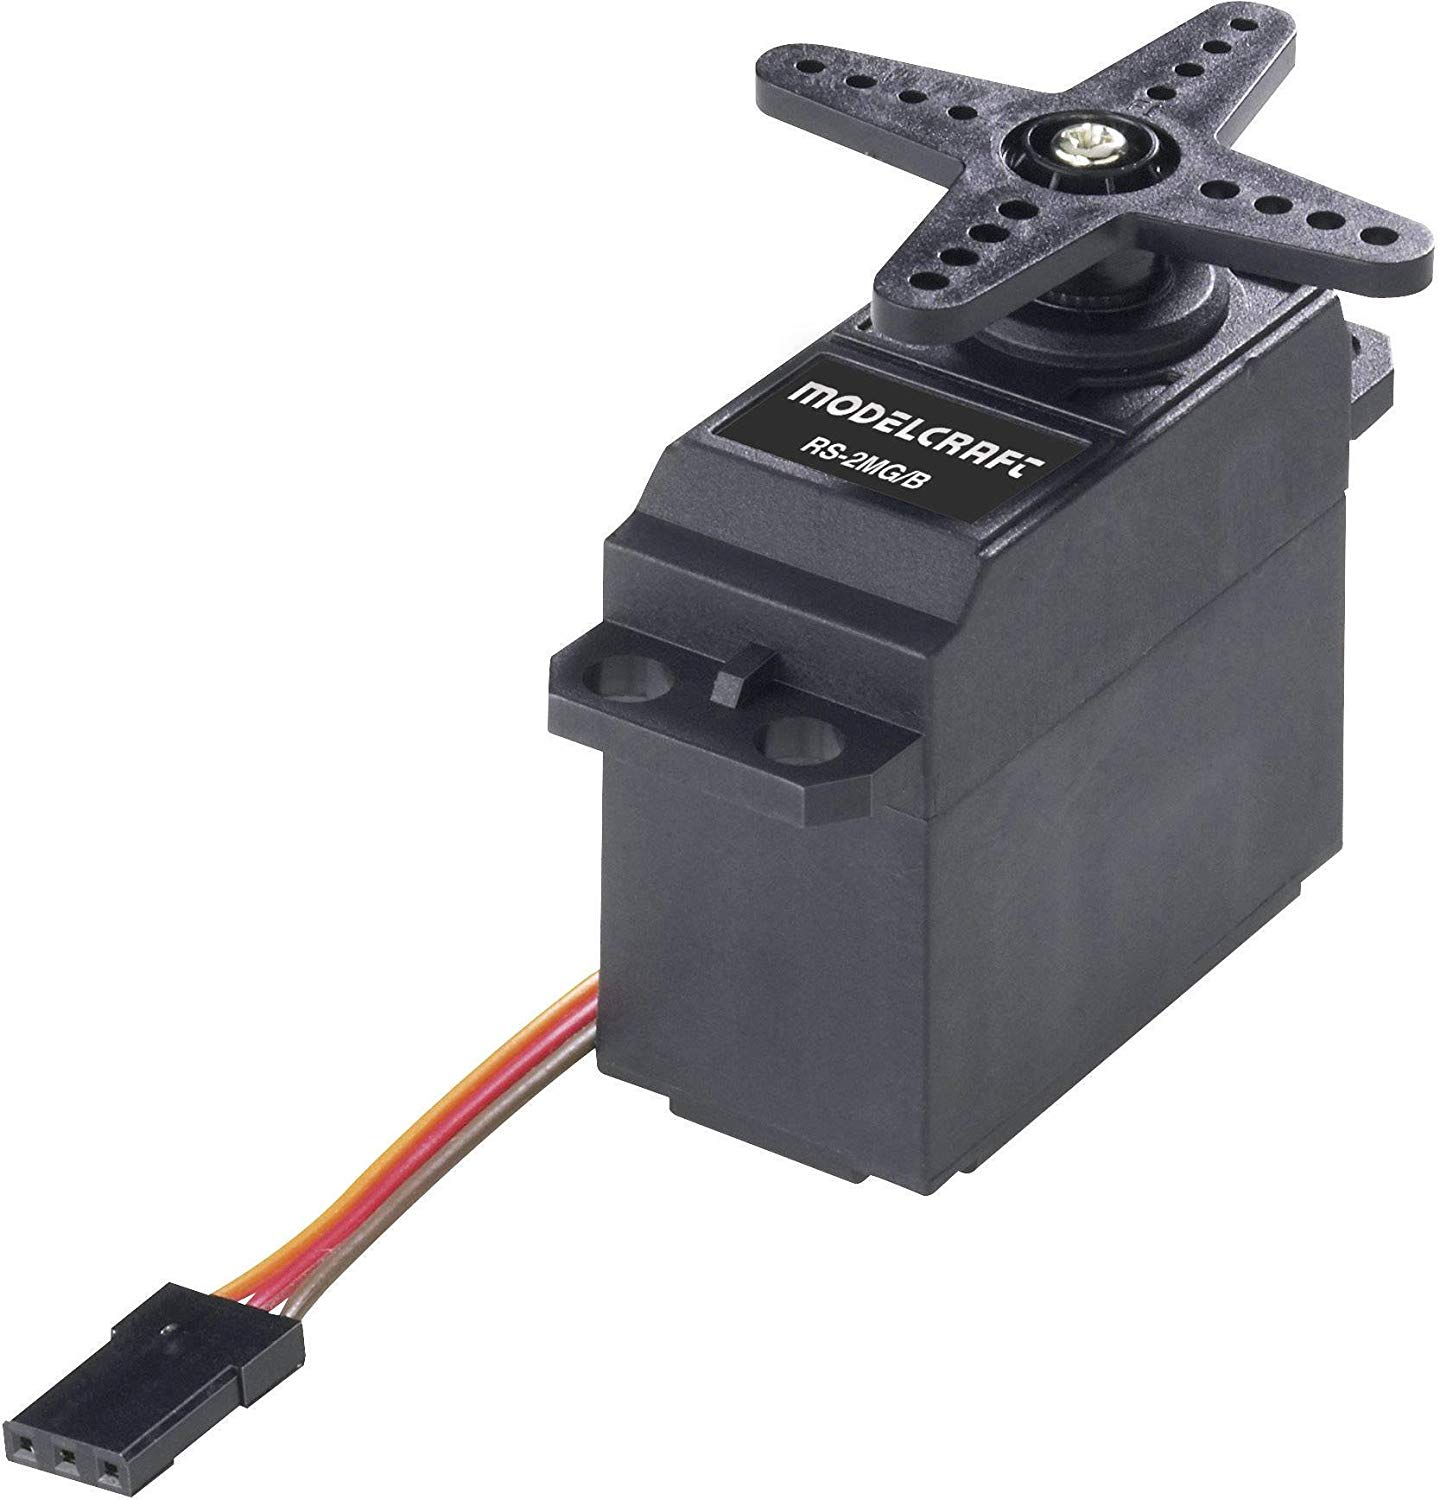
\includegraphics[scale=0.1]{imagenes/servo.jpg}
  \end{center}
  \caption{Imagen de un servomotor.}
  \label{figure:servomotor:}
\end{figure}

Un servomotor se compone de un motor, un circuito de control, un potenciómetro y un conjunto de engranajes. Los cuales se caracterizan por un consumo energético muy reducido.\\

Podemos definir un servomotor como un motor al que se le ha añadido un sistema de control, un potenciómetro y un conjunto de engranajes. Con anterioridad los servomotores no
permitían que el motor girara 360 grados, solo aproximadamente 180; sin embargo, hoy en día existen servomotores en los que puede ser controlada
su posición y velocidad en los 360 grados. Los servomotores son comúnmente usados en modelismo para controlar y dotar de movimiento multitud de elementos.\\

En cuanto al conexionado, los servomotores poseen tres cables de conexión externa, alimentación, tierra y control. Mediante éste último indicamos el ángulo al cuál queremos llegar. 
Un servomotor normal tiene un movimiento angular de 0 a 180º, caso del utilizado en este proyecto. El ángulo está determinado por la duración de un pulso. El servomotor 
espera ver un pulso cada 20 milisegundos. La longitud del pulso determinará el giro que ha de realizar el motor. Un pulso de 1.5 ms hará que el motor se posicione en la posición 
neutra, a 90º respecto al eje. En caso contrario, si el pulso es menor de 1.5 ms,  el motor se acercará a 0º, y si el pulso es mayor de 1.5ms, el eje se acercará a los 180 grados.\\

Inicialmente se pensó en utilizar un dispositivo de este tipo para el control de la dirección del vehículo pero debido a que el chasis utilizado ya incorporaba un motor de continua tradicional
que cumplía muy bien su cometido, éste ha sido descartado. Dicho servomotor podría ser utilizado para dotar de movimiento de elevación, por ejemplo a la cámara que incorpora el vehículo tal y como
se recoge en la sección \ref{sec:mejoras_futuras} correspondiente a mejoras futuras.\\

\subsection{Interconexión de elementos}

En el presente punto se recogen todos aquellos puntos de interés referentes a la interconexión de elementos utilizados, los cuales quedaron descritos en la sección \emph{Tecnologías hardware}
\ref{sec:tecnologias-hardware} junto con sus especificaciones.\\

Comenzando por el módulo central del sistema, la placa Raspberry Pi Model B+\footnote{ Todo lo referente a la utilización de los puertos de Entrada/Salida, puesta en funcionamiento y
utilización de la placa Raspberry Pi se encuentra disponible en el manual de usuario \cite{book:Raspberry} elaborado por uno sus creadores. }, dispone de una serie de pines denominados GPIO (General Purpose Input/Output) es, como su propio nombre indica, 
un sistema de E/S (Entrada/Salida) de propósito general, es decir, una serie de conexiones que se pueden usar como entradas o salidas para usos múltiples. Estos pines se encuentran en todos
los modelos de Raspberry Pi.\\

Comentar que debido a la incorporación de una placa Arduino no se han utilizado ninguno de los puertos GPIO que la Raspberry Pi ofrece a pesar de que hubiesen resultado perfectamente 
funcionales y encontrándose disponibles para cualquier ampliación que se desee realizar con posterioridad. Se ha optado por dejar a la placa tan solo como unidad central de 
procesamiento, conexión del vehículo con una red de internet y transmisión de los datos capturados al servidor y escucha de comandos recibidos.\\

Pero existe una problemática y es que no podemos conectar directamente los pines de salida de nuestra placa Arduino directamente a los motores. Esto es debido a
que la placa no dispone de potencia suficiente para mover actuadores. De hecho, la función de la placa no debe ser ejecutar acciones sino mandar ejecutar acciones a drivers que
realicen el trabajo pesado.\\

\subsection{Driver motores}
\label{sec:drivers}

Un driver motor es un dispositivo, o grupo de dispositivos, que se utilizan para controlar de una manera predeterminada el funcionamiento de un motor eléctrico. El control 
se consigue mediante unas señales de entrada, ya sean analógicas o bien digitales, con las que 
conseguimos:

\begin{itemize}
 \item Seleccionar el sentido de giro del motor: gracias a la utilización de un driver, podemos 
elegir el sentido horario o anti horario del motor de manera muy simple.
\item Regular la velocidad mediante el uso de una señal PWM, el driver permitirá regular la velocidad de variación de un motor DC
\item Permite la alimentación necesaria para el correcto funcionamiento del motor.
\item Protección del circuito: al incluir un driver en el circuito, nos ofrece protección contra 
posibles sobrecargas y fallas que puedan aparecer.
\end{itemize}

Para ello empleamos el L298N, un controlador (driver) de motores integrado en un módulo, el cual nos permite encender y controlar dos motores de corriente continua desde una Raspberry Pi, Arduino o
cualquier placa similar, variando tanto la dirección como la velocidad de giro.\\

La corriente máxima que el L298N es capaz de suministrar a los motores es, en teoría, 2A por salida, permitiendo alcanzar hasta los 3A de pico, y una tensión de alimentación de 3V
a 35V. Sin embargo, el L298N tiene una eficiencia energética extremadamente baja. La electrónica supone una caída de tensión de unos 3V, es decir, la tensión que recibe el motor
es unos 3V inferior a la tensión de alimentación, todo ello unido a la gran cantidad de calor que disipa el driver.\\

Estas pérdidas se traducen en que, a efectos prácticos, es difícil que podamos obtener más de 0.8-1A por fase sin exceder el rango de temperatura de funcionamiento.\\

El L298N tiene la ventaja de que incorpora protecciones contra efectos que pueden producirse al manejar motores de corriente continua. Dispone de protecciones contra situaciones
de elevada intensidad, temperatura, y diodos de protección contra polaridades incorrectas.\\

Dicho módulo cuenta con todos los componentes necesarios para funcionar sin necesidad de elementos adicionales entre los que incluye un regulador \textbf{LM7805} que suministra 5V
a la parte lógica del integrado L298N. Además cuenta con jumpers de selección para habilitar cada una de las salidas del módulo (A y B). La \textbf{salida A} esta conformada
por \textbf{OUT1} y \textbf{OUT2} y la \textbf{salida B} por \textbf{OUT3} y \textbf{OUT4}. Los pines de habilitación 
son \textbf{ENA} y \textbf{ENB} respectivamente.\\

Los pines \textbf{IN1}, \textbf{IN2}, \textbf{IN3} y \textbf{IN4}; son los pines de entrada donde se conectan a pines digitales de Arduino para poder controlar el motor.\\

La alimentación del driver es variable existiendo dos modos de funcionamiento, ya que dispone de un regulador de tensión de 5v incorporado. Cuando el jumper de selección de 5V se
encuentra activo, el módulo permite una alimentación de entre 6V a 12V DC. Como el regulador se encuentra activo, el pin marcado como +5V tendrá un voltaje de 5V DC.
Este voltaje se puede usar para alimentar la parte de control del driver ya sea un micro-controlador o un Arduino no debiendo superar los 500 mA.\\

Cuando el jumper de selección de 5V se encuentra inactivo, el driver permite una alimentación de entre 12V a 35V DC. Como el regulador no está funcionando, tendremos que conectar el pin de +5V a una tensión de 5V para alimentar la parte 
lógica del L298N.\\

En  este  caso  se  utilizará una fuente de 11,1V manteniendo el jumper activo, y así alimentar la parte de control del driver.\\

En la figura \ref{diagrama:L298N-salidas} se muestra el módulo empleado con sus diferentes pines al detalle.\\

\begin{figure}[H]
  \begin{center}
    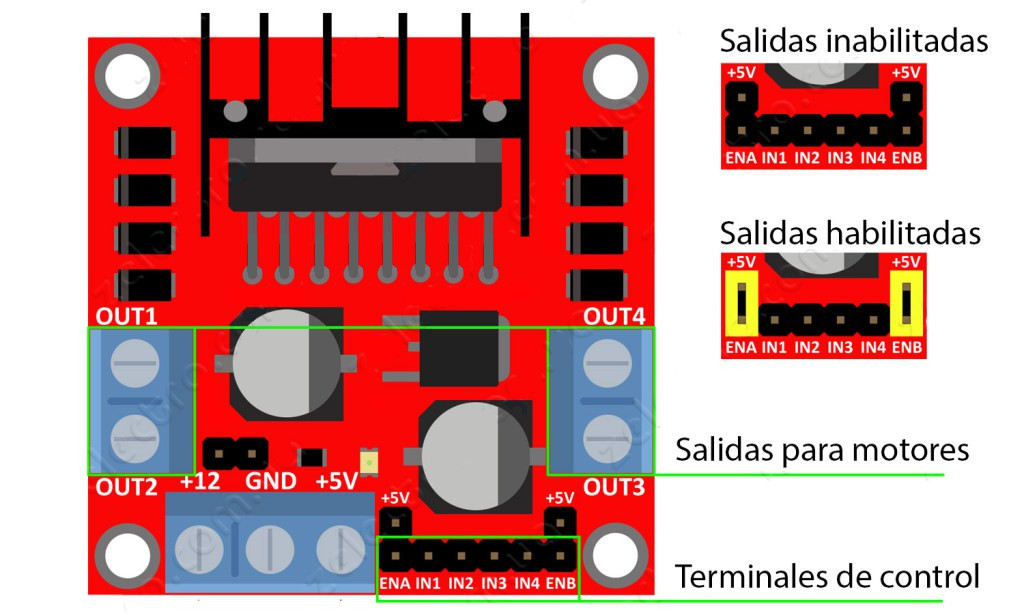
\includegraphics[scale=2]{imagenes/L298N-conexiones.jpg}
  \end{center}
  \caption{Pines de entrada/salida del módulo L298N empleado.}
  \label{diagrama:L298N-salidas}
\end{figure}

Centrándonos a un nivel más bajo, dicho módulo incorpora, lo que conocemos en electrónica como puente en H, el cual es un circuito electrónico que permite cambiar el sentido de giro de los 
motores de corriente continua. Este circuito lo componen cuatro interruptores, los cuales pueden ser mecánico o electrónicos (diodos, transistores...) de forma que,
en función de cuales se abran o cierren, permitirán cambiar el sentido de alimentación de un motor.  Los podemos encontrar como circuitos integrados, pero también se
pueden crear con componentes discretos.\\

\begin{figure}[H]
  \begin{center}
    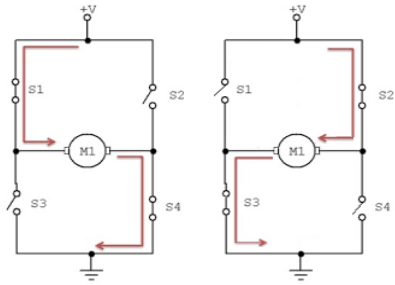
\includegraphics[scale=0.7]{imagenes/esquema_puente_h.png}
  \end{center}
  \caption{Diagrama de funcionamiento del puente H.}
  \label{esquema:funcionamiento_puente_h}
\end{figure}

El funcionamiento de un puente H es bastante simple. Siguiendo la Figura \ref{esquema:funcionamiento_puente_h} podemos observar que, cuando se cierran los interruptores \textbf{S1} y \textbf{S4}, y se abren \textbf{S2} y \textbf{S3}, se aplica una tensión positiva en bornes del motor, así 
que este gira en un sentido y cuando se abren los interruptores \textbf{S1} y \textbf{S4} y se cierran \textbf{S2} y \textbf{S3}, se invierte la tensión en bornes del motor, haciendo que el motor gire en sentido contrario.\\

Y, por contra, si todos los interruptores están abiertos el motor no girará. \\

Para el caso del proyecto, hemos empleado utilizado las salidas para la conexión de dos motores, empleando así todas las que el driver proporciona. Una de ellas para traccionar
el vehículo y la segunda para el accionamiento de la dirección.\\

Se ha optado finalmente por emplear un motor DC para la dirección debido que el chasis empleado para la construcción del robot ya lo traía así incorporado y se ha decidido reutilizar.
De igual modo se podría haber empleado un servomotor para el accionamiento de la dirección, pero debido a una mayor simplicidad en el montaje y puesto que el motor ya incorporado
dispone de una mejor sujeción al chasis así se ha decidido.\\

\subsection{Motores}

En la figura \ref{img:sistema_direccion} se muestra el motor de dirección empleado junto con el sistema de topes de recorrido que incorpora.\\


\begin{figure}[H]
  \begin{center}
    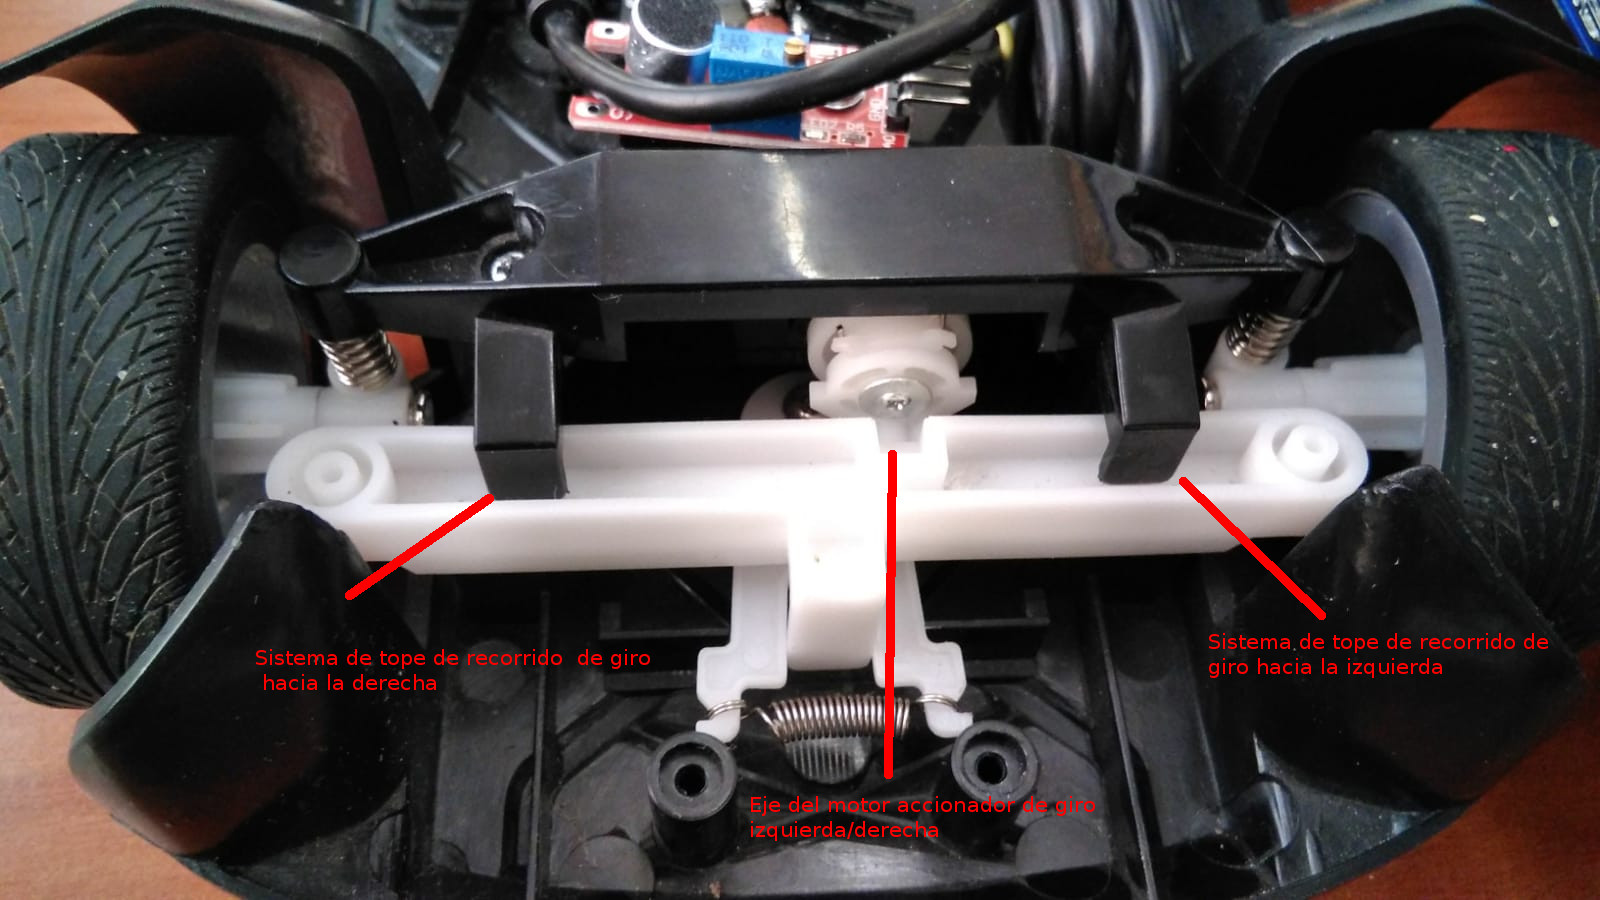
\includegraphics[scale=0.2]{imagenes/robot/motor-direccion.jpg}
  \end{center}
  \caption{Sistema de accionamiento de la dirección.}
  \label{img:sistema_direccion}
\end{figure}

Motor de tracción del vehículo situado en su parte trasera, figura \ref{img:motor_traccion}.

\begin{figure}[H]
  \begin{center}
    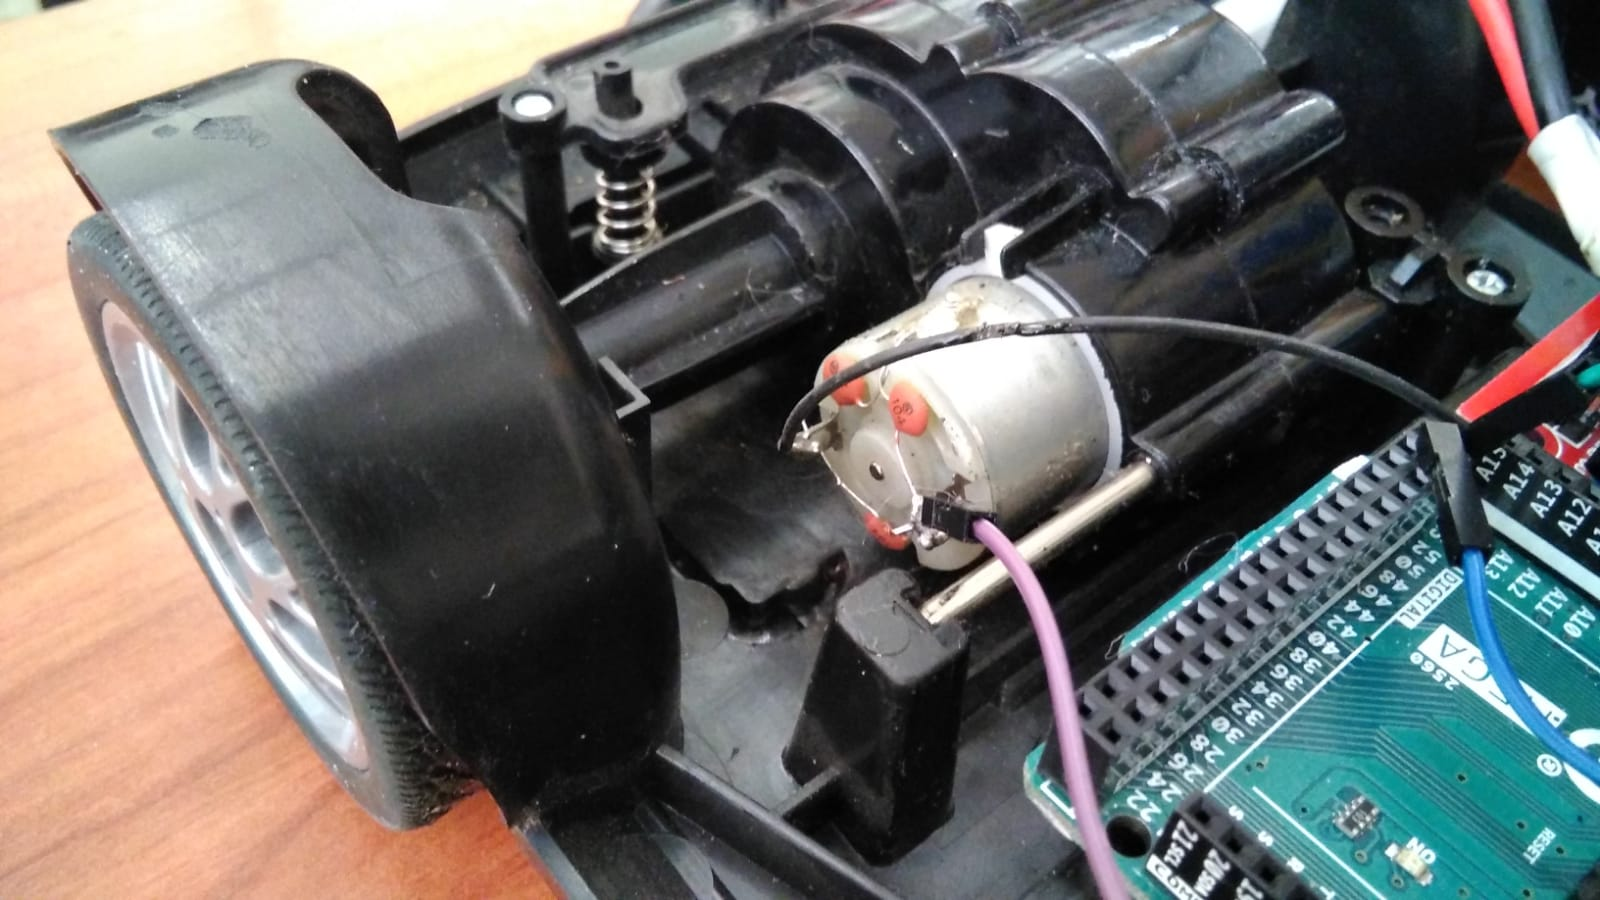
\includegraphics[scale=0.2]{imagenes/robot/motor-traccion.jpg}
  \end{center}
  \caption{Vista del motor de tracción.}
  \label{img:motor_traccion}
\end{figure}


\subsubsection{Conexionado}

\begin{figure}[H]
  \begin{center}
    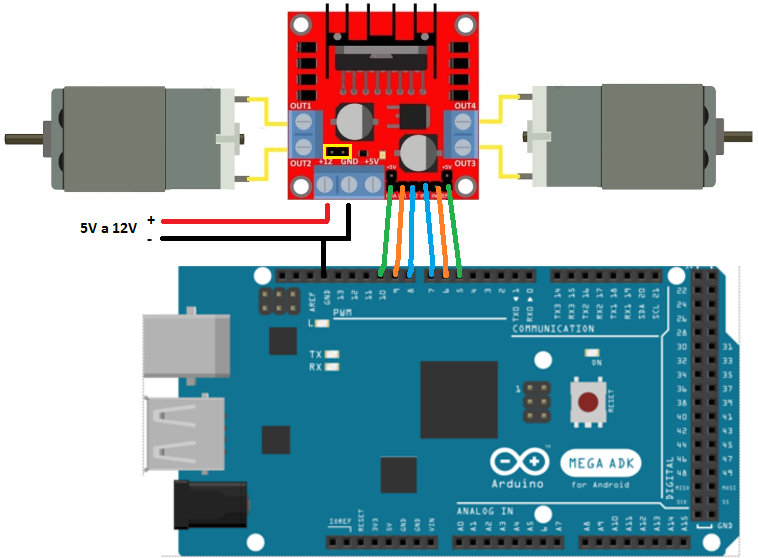
\includegraphics[scale=0.4]{imagenes/L298N_conexionado.png}
  \end{center}
  \caption{Conexionado del conjunto motores, driver y Arduino.}
  \label{img:motor_traccion}
\end{figure}


\section{Alimentación}
\label{sub:alimentación}

Resulta de vital importancia el dotar de energía nuestro proyecto siendo una de las partes más importantes y críticas del mismo. La selección de los componentes adecuados
requiere una realización previa de estudio de las necesidades que se desean cubrir puesto que una decisión equivocada puede implicar un defectuoso
comportamiento del conjunto.\\

Por tanto, cuando se escoja la batería se deben tener en cuenta los siguientes puntos:\\

\begin{enumerate}

 \item \textbf{Consumo máximo del robot:} A partir de las características de todos los
componentes, se tiene que mirar cuál será su consumo máximo (motores a pleno
rendimiento, electrónica consumiendo al máximo, etc.), y una vez determinado,
buscar una fuente de alimentación que sea capaz de proporcionar esta corriente.

\item \textbf{Pico de consumo máximo:} Cuando un motor se pone en marcha, se origina un
pico de consumo por la resistencia que tiene a moverse. Este pico será mayor
cuanta más velocidad se da y/o mayor carga se desee mover. La batería debe ser
capaz de proporcionar estos picos y no ver comprometido su funcionamiento. Si no
fuera capaz, provocaría una bajada de tensión para proporcionar esta corriente, y
podría apagar el resto de la electrónica. Este valor se suele encontrar en las
baterías como C. Por ejemplo, si la batería es de 1000 mAh con un C de 10, podrá
suministrar picos de hasta 10000 mA, o lo que es lo mismo, 10 Amperios.


\item \textbf{Capacidad:} Todas las baterías recargables dan una cifra de carga, se suele
expresar en Ah (Amperios/hora) o mAh (miliamperios/hora). Esta cifra indica
cuantos amperios/hora es capaz de dar la batería antes de descargarse. Por tanto,
si el consumo es de 10 mA y la batería es de 100 mAh, el equipo podrá estar en
marcha durante 10 horas, si por el contrario el consumo es de 100mA y la batería
es de 10mAh, el equipo solo podrá estar en funcionamiento 6 minutos.

\item \textbf{Voltaje:} Este valor dependerá de las tensiones que se necesiten en el circuito, ya
sea por parte del motor, o por parte de la electrónica de control.

\end{enumerate}

En ocasiones, muchos de los diseños de los robots se realizan incorporando dos baterías separadas. Utilizando esta configuración separamos la
parte digital (sistema de control y sensado) de la parte analógica (motores). Los motores son muy ruidosos, y a través de la alimentación pueden inducir ruidos
al resto de circuitería. En el mejor de los casos el sistema será lo suficientemente robusto para soportar estos problemas, pero muchas
veces este ruido falsea las medidas, o hasta puede provocar que la parte del control se resetee.\\

Por esta razón, se ha optado por el uso de dos baterías para la alimentación del conjunto. Una para dotar de energía a la placa de control y otra para la alimentación de los 
motores debido a la gran cantidad de energía que éstos demandan y su elevado consumo.\\

Para la alimentación de la placa Raspberry Pi, se ha optado por la utilización de una batería de Litio desarrollada específicamente para su uso con este modelo de placas el cual permite una integración
perfecta. Dicho módulo de alimentación queda descrito en la subapartado correspondiente de herramientas utilizadas \ref{componente:bateria-expansion}.\\

Imagen de la Raspberry Pi junto con su módulo de expansión de batería:

\begin{figure}[H]
  \begin{center}
    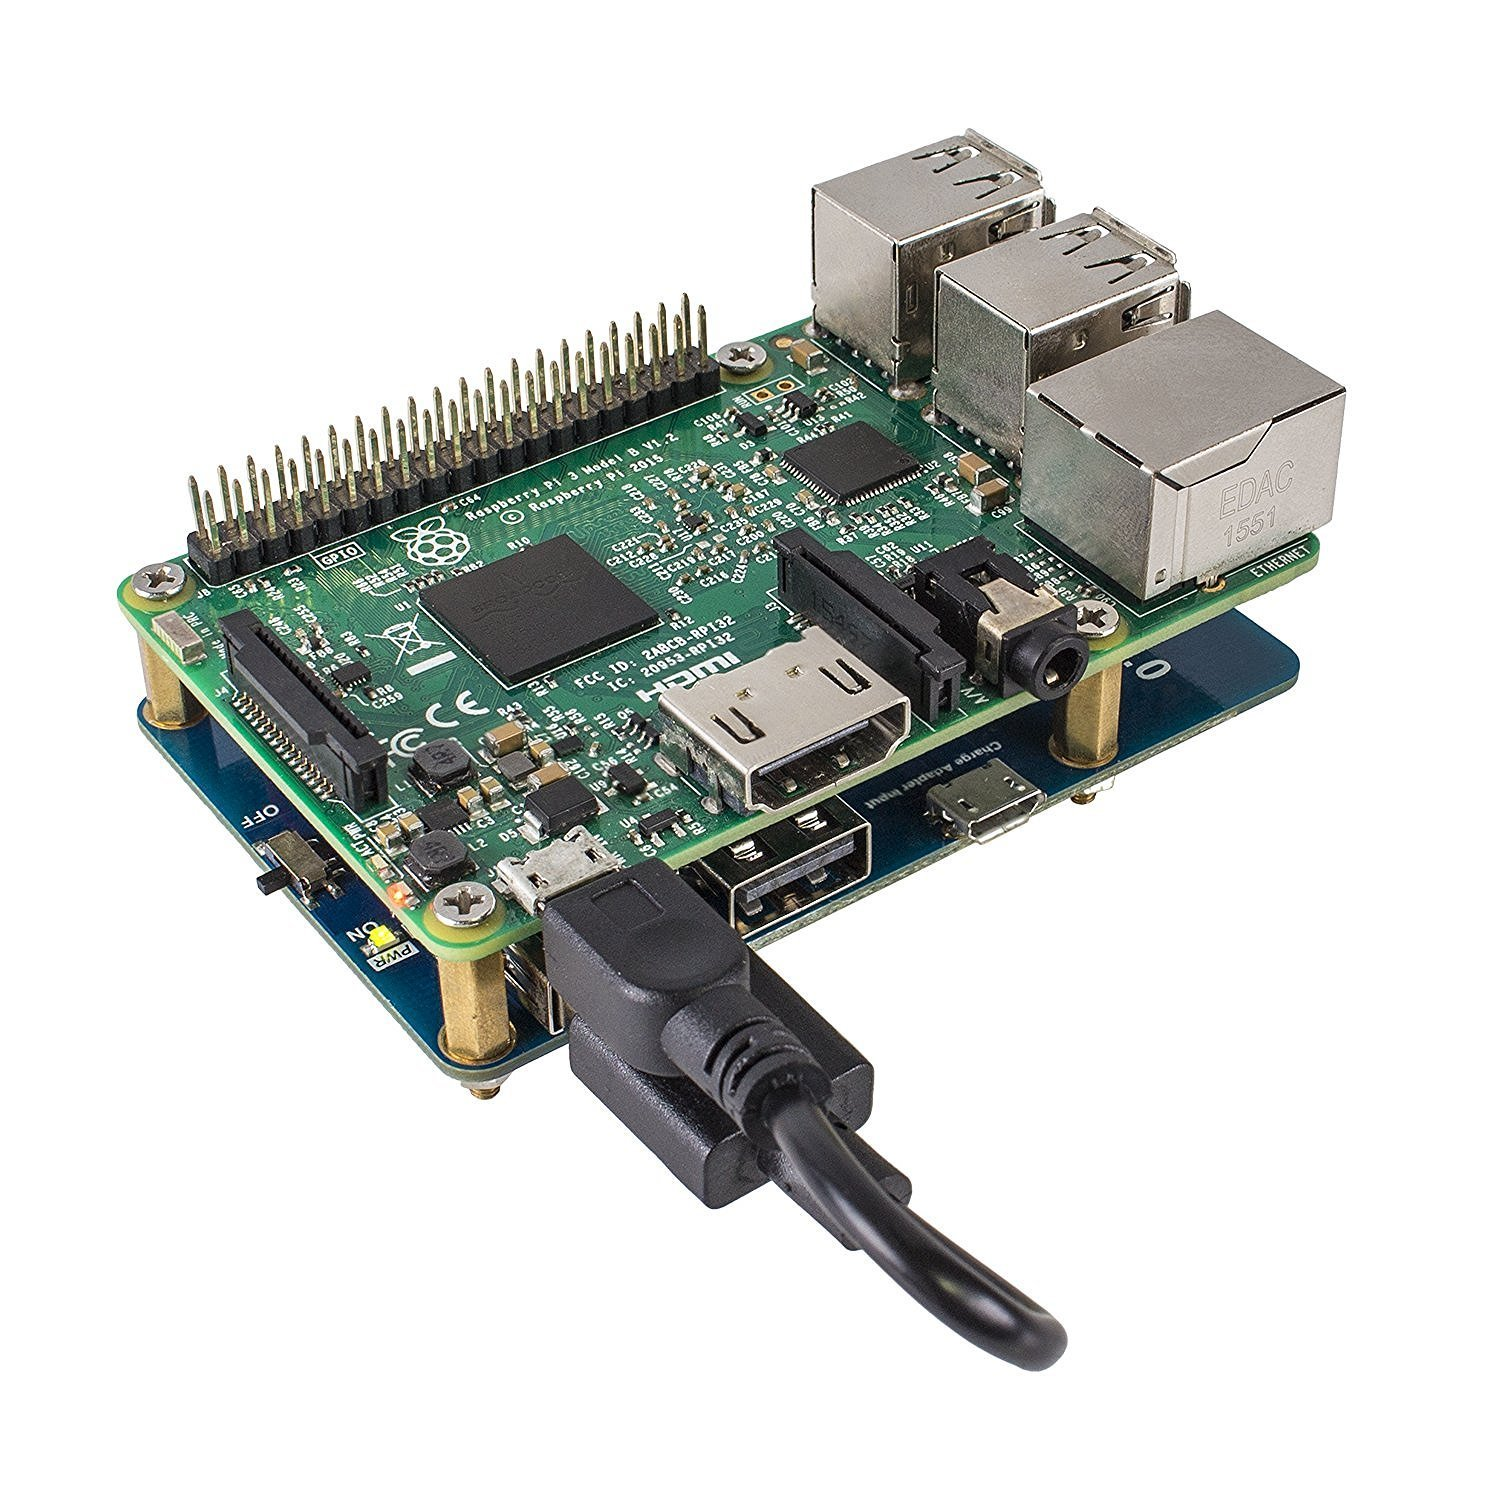
\includegraphics[scale=0.10]{imagenes/modulo-expansion-rpi.jpg}
  \end{center}
  \caption{Conjunto Raspberry Pi y módulo de expansión de alimentación.}
  \label{figura:rpi-modulo-bateria}
\end{figure}

Imagen de la batería LiPo para la alimentación de los motores:

\begin{figure}[H]
  \begin{center}
    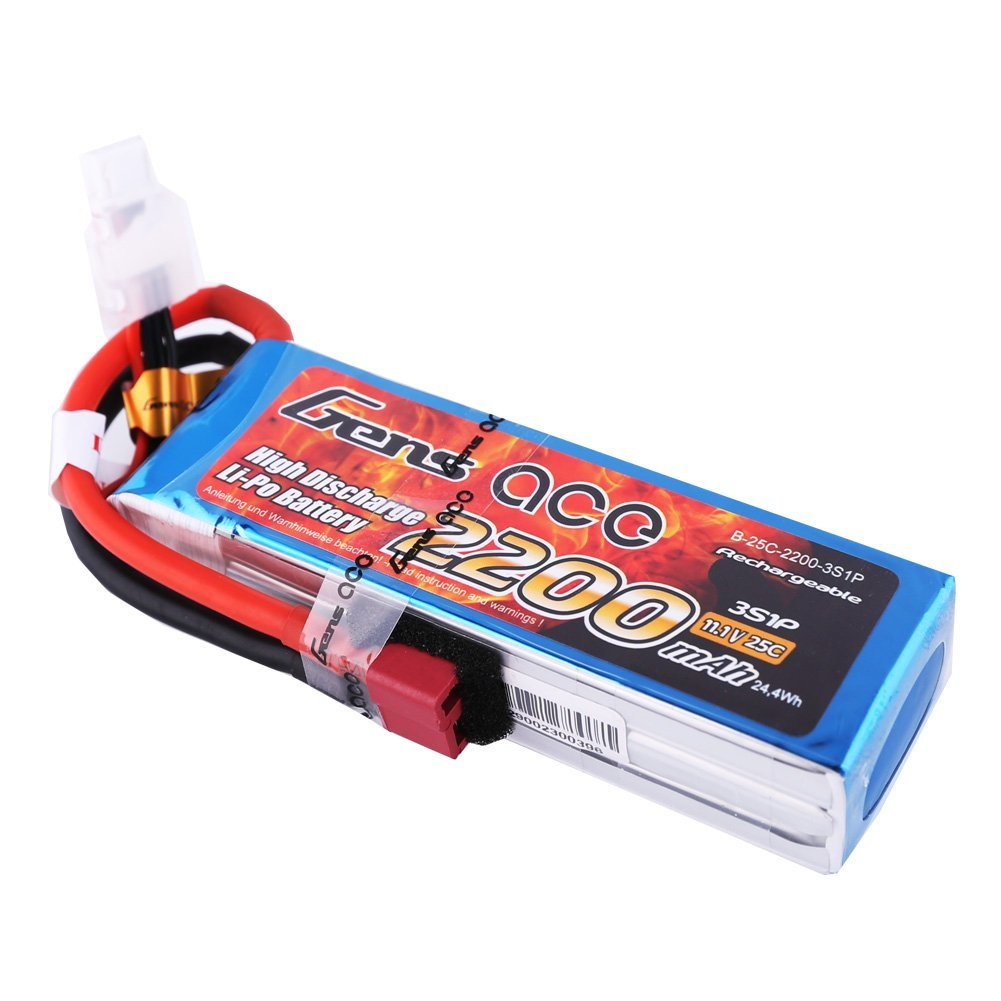
\includegraphics[scale=0.15]{imagenes/robot/bateria.jpg}
  \end{center}
  \caption{Batería LiPo que alimenta los motores.}
  \label{figura:rpi-modulo-bateria}
\end{figure}


\begin{figure}[H]
  \begin{center}
    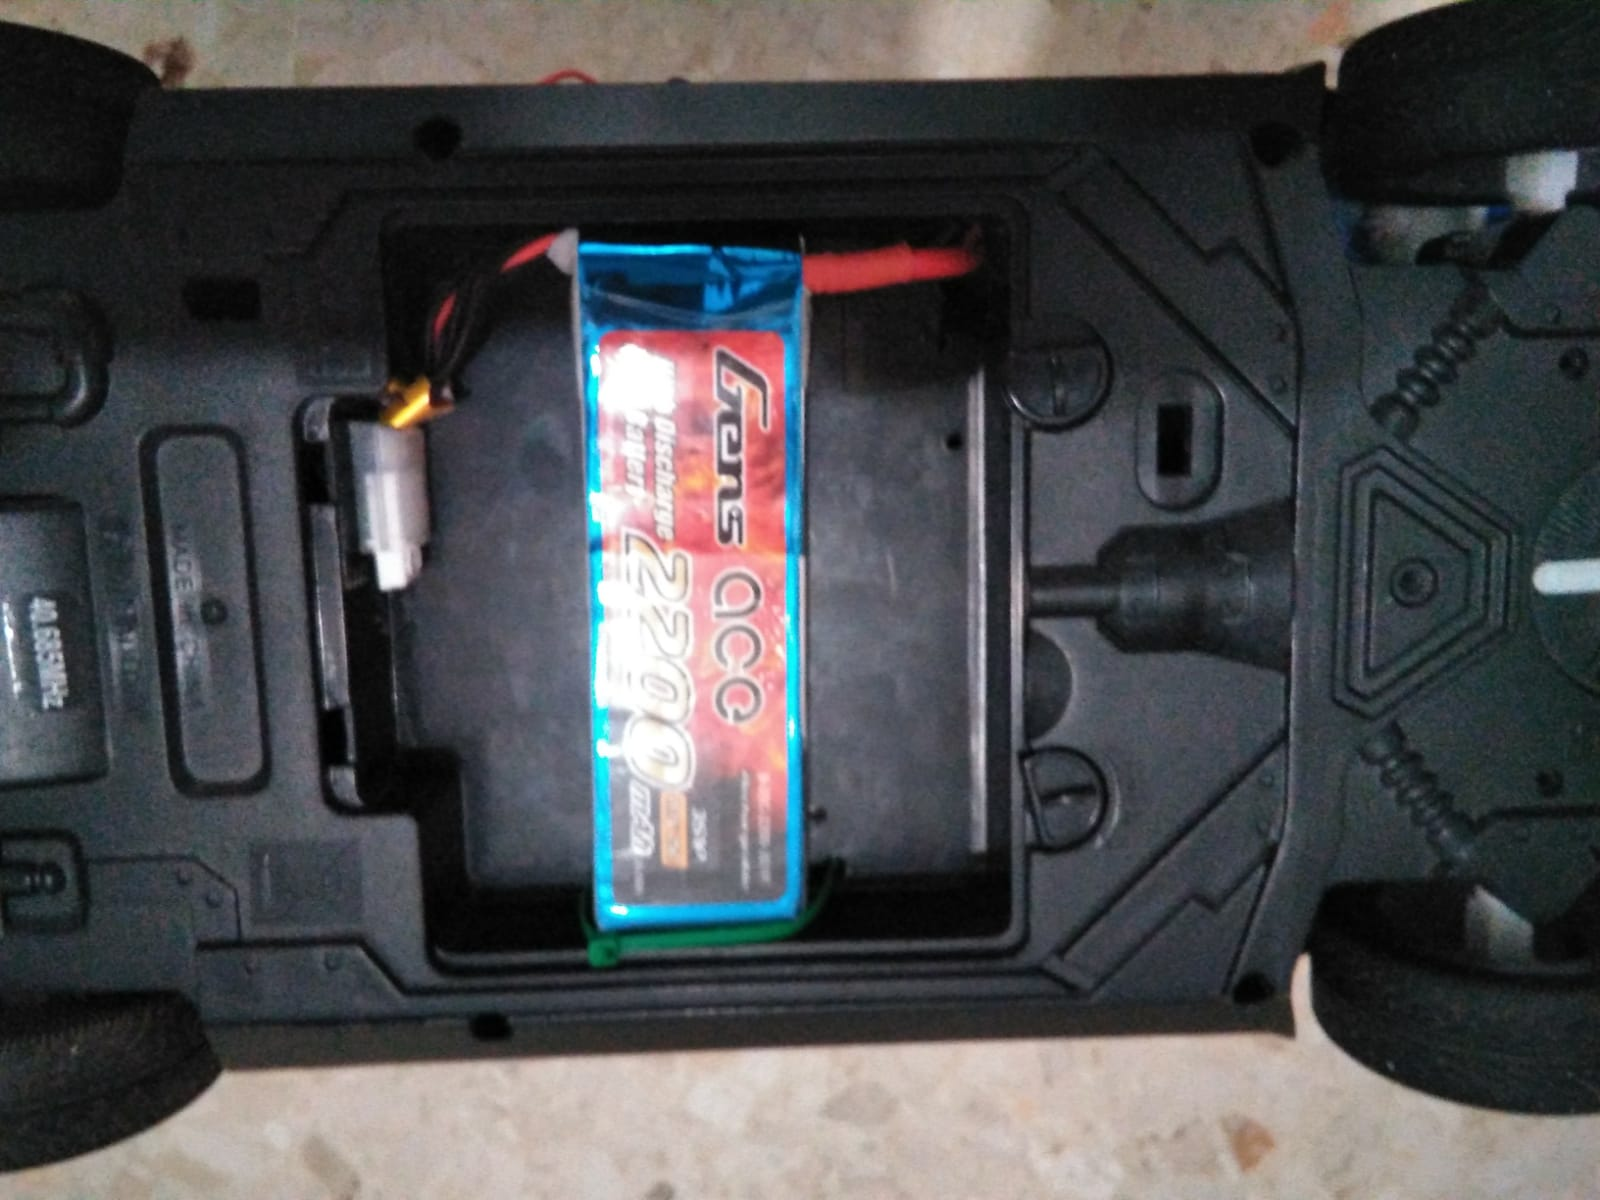
\includegraphics[scale=0.15]{imagenes/robot/alojamiento_bateria.jpg}
  \end{center}
  \caption{Alojamiento de la batería LiPo.}
  \label{figura:rpi-modulo-bateria}
\end{figure}



\subsubsection{ Alimentación USB/Protoboard }

Para alimentar la protoboard sin tener que modificar un cable USB, se ha decidido utilizar una pequeña tarjeta que se conecta en los carriles de tensión de la tarjeta Protoboard, y
proporciona los 5 V de entrada del USB (o de un conector Jack) a las líneas de alimentación de la protoboard. Además este dispositivo integra un interruptor, que permitirá activar y
desactivar los motores, y puede regular la tensión a 3,3 Voltios.\\

\begin{figure}[H]
  \begin{center}
    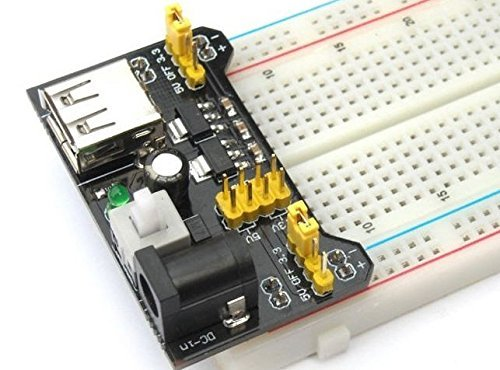
\includegraphics[scale=0.3]{imagenes/alimentador_usb_protoboard.jpg}
  \end{center}
  \caption{Adaptador de entrada USB a protoboard.}
  \label{figura:alimentador_usb_protoboard}
\end{figure}

La alimentación de este módulo se puede realizar de dos formas: mediante el uso de una pila o batería, o mediante un cable USB. Para saber que está correctamente alimentado, este 
dispositivo incorpora un indicador led que avisará si se está usando de forma correcta. Otra característica importante de este módulo, es la posibilidad de elegir la tensión de
salida que proporciona, pudiendo seleccionar una alimentación de 5V y otra de 3,3V a la vez.\\

En la Figura \ref{figura:alimentador_usb_protoboard_esquema} puede verse el esquema eléctrico del módulo.\\

\begin{figure}[H]
  \begin{center}
    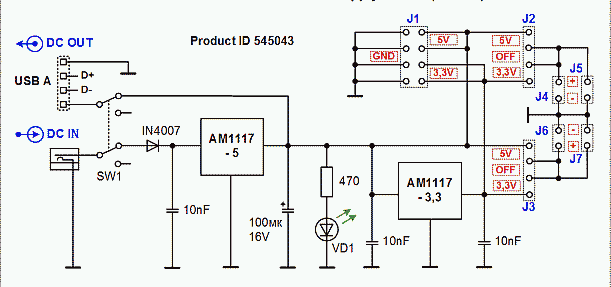
\includegraphics[scale=0.5]{imagenes/esquema_alimentador_protoboard.png}
  \end{center}
  \caption{Esquemático del adaptador de entrada USB a protoboard.}
  \label{figura:alimentador_usb_protoboard_esquema}
\end{figure}

Siguiento el esquema \ref{figura:alimentador_usb_protoboard_esquema} Podemos diferenciar los distintos componentes según su funcionalidad dentro del módulo:

\begin{itemize}
 \item \textbf{Alimentación USB:} Esta entrada solo se utiliza para la alimentación de 5 voltios mediante un conector USB hembra.
 Los pines centrales, D+ y D- no están conectados a ningún elemento, por lo que no puede recibir datos.

 \item \textbf{Alimentación externa:} Se trata de un conector tipo Jack hembra al que se le puede colocar cualquier tipo de batería
 o pila que se encuentre entre los rangos de 6 y 12V permitidos por el módulo.
 
 \item \textbf{AM1117-5 y AM1117-3.3:} Son los dos reguladores de tensión que incorpora el módulo MB102 para regulación de tensión de salida hasta los valores 
 5 y 3,3V respectivamente.
 
 \item \textbf{ Diodos y condensadores} También incorpora una serie de diodos zener \footnote{El diodo Zener es un diodo de silicio altamente dopado​ ideado para que funcione en las zonas de rupturas. Estos tipos de diodos
 resultan fundamentales en los reguladores de tensión proporcionando valores prácticamente constantes con independencia ante variaciones de tensión, resistencia y temperatura. } 
 de portección ante posibles inversiones de polaridad junto con un diodo led para comprobar el correcto funcionamiento del módulo.
 
 \item \textbf{SW1:} Botón cuya finalidad es encender o apagar el módulo de alimentación.
 
 \item \textbf{J1:} Serie de pines en los cuales se tiene una tensión de 5V y 3.3V para la conexión de los diferentes elementos. De los ocho pines que dispone, cuatro pines son
 de GND, dos pines son de 5V y los otros dos pines restantes son de 3.3V.
 
 \begin{figure}[H]
  \begin{center}
    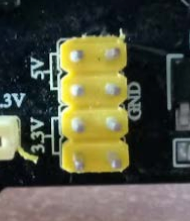
\includegraphics[scale=0.5]{imagenes/usb_board_pines.png}
  \end{center}
  \caption{Vista del conector J1.}
  \label{figura:conector_usb_board_j1}
\end{figure}

  \item \textbf{J2 y J3:} Pines para la selección de la tensión de salida del módulo. Para seleccionar la tensión debemos conectar un jumper\footnote{En electrónica y en particular en informática, un jumper
   es un elemento utilizado para interconectar dos terminales de manera temporal sin tener que efectuar una operación que requiera herramienta adicional cerrando circuito eléctrico del que forma parte. } entre los pines en función de la
  tensión deseada.

   \begin{figure}[H]
  \begin{center}
    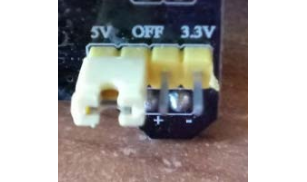
\includegraphics[scale=0.5]{imagenes/usb_board_vout.png}
  \end{center}
  \caption{Vista del conector J2 y J3.}
  \label{figura:conector_usb_board_vout}
\end{figure}

\item \textbf{J4 y J5:} Pines que incorpora el modulo en su parte inferior para la conexión de este en 
una protoboard.

   \begin{figure}[H]
  \begin{center}
    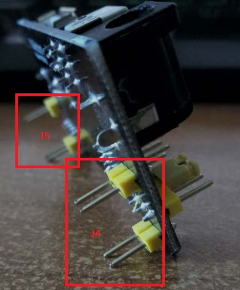
\includegraphics[scale=0.5]{imagenes/pin_usb_board.png}
  \end{center}
  \caption{Vista del conector J4 y J5.}
  \label{figura:conector_usb_board}
\end{figure}
  
\end{itemize}


\subsection{Interconexión entre módulos y fijación}

La conexión entre los diferentes módulos se realiza utilizando cables USB, y cables de interconexión entre la Raspberry/Arduino con la protoboard utilizándose la técnica
conocida como Wire-Wrap o cables tipo jumper-wire.\\

\begin{figure}[H]
  \begin{center}
    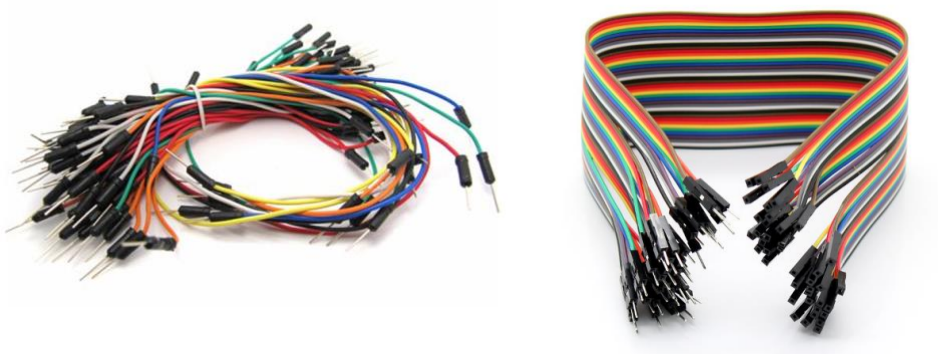
\includegraphics[scale=0.3]{imagenes/cables_interconexion.png}
  \end{center}
  \caption{Cables de interconexión para protoboard.}
  \label{figura:cables_interconexion}
\end{figure}

Para la fijación de los diferentes módulos al chasis se ha empleado tornillería y bridas, éstas últimas para mantener el cableado más ordenado.\\

\subsection{Conexionado general}

La siguiente imagen \ref{vista-conexiones} muestra una visión general de la disposición de todos los elementos que conforman el vehículo junto con sus conexiones:\\


\begin{figure}[H]
  \begin{center}
   \includegraphics[scale=0.3]{diagramas/conexionado_etiquetas_general.png}
  \end{center}
  \caption{Vista del conexionado general del robot.}
  \label{vista-conexiones}
\end{figure}

La Tabla \ref{table:pines_utilizados} muestra los pines utilizados, modo de configuración y propósito en la placa Arduino:\\

\begin{table}[H]
  \begin{center}
    \begin{tabular}{|p{2.5cm}|p{4cm}|p{6cm}|}
      \hline
      {\textbf{Pin Arduino}} & \textbf{ Modo } & \textbf{ Pin destino }\\
      \hline
      {\textbf{ A0 }} & { INPUT } & { Entrada analógica SHARP GP2D12 }  \\
     \hline
      {\textbf{ D48 }} & { INPUT } & { Entrada digital del Buzzer } \\
      \hline
      {\textbf{ D38 }} & { INPUT } & {  Entrada digital del micrófono KY-038 } \\
      \hline
      {\textbf{ A2 }} & { INPUT } & { Entrada analógica del sensor de llama YG1006 } \\
      \hline
      {\textbf{ D4 }} & { OUTPUT } & { TRIG del sensor HC-SR04 trasero derecho } \\
      \hline
      {\textbf{ D5 }} & { INPUT } & { ECHO del sensor HC-SR04 trasero derecho} \\
      \hline
      {\textbf{ D7 }} & { OUTPUT } & { TRIG del sensor HC-SR04 trasero izquierdo } \\
      \hline
      {\textbf{ D2 }} & { INPUT } & { ECHO del sensor HC-SR04 trasero izquierdo } \\
      \hline
      \end{tabular}
  \end{center}
\end{table}      
      

\begin{table}[H]
  \begin{center}
    \begin{tabular}{|p{2.5cm}|p{4cm}|p{6cm}|}
      \hline
      {\textbf{ D3 }} & { INPUT } & { Entrada digital del sensor DTH11 } \\
      \hline      
      {\textbf{ A1 }} & { OUTPUT } & { Entrada analógica del fotoresistor } \\      
      \hline	  
      {\textbf{ D35 }} & { INPUT } & { Entrada analógica del sensor de gas MQ-2 fotoresistor } \\            
      \hline
      {\textbf{ D13 }} & { OUTPUT - PWM } & { Entrada ENA del driver L298N para control de tracción } \\
      \hline
      {\textbf{ D12 }} & { OUTPUT } & { Entrada IN3 del driver L298N para control de tracción } \\
      \hline
      {\textbf{ D11 }} & { OUTPUT } & { Entrada IN4 del driver L298N para control de tracción } \\      
      \hline
      {\textbf{ D10 }} & { OUTPUT - PWM } & { Entrada ENB del driver de motores L298N para control de dirección } \\
      \hline
      {\textbf{ D9 }} & { OUTPUT } & { Entrada IN1 del driver L298N para control de dirección } \\
      \hline
      {\textbf{ D8 }} & { OUTPUT } & { Entrada IN2 del driver L298N para control de dirección } \\      
      \hline
      {\textbf{ D6 }} & { OUTPUT } & { Entrada positiva de los leds de iluminación del vehículo } \\      
      \hline
      {\textbf{ D37 }} & { OUTPUT } & { Entrada positiva del puntero láser del vehículo } \\      
     \hline   
    \end{tabular}
  \end{center}
\caption{ Pines utilizados en la placa Arduino Mega. }
\label{table:pines_utilizados}
\end{table}

La Figura \ref{fig:esquematico-conexiones} muestra el esquemático global de SensorRS.\\

\begin{figure}[H]
  \hspace*{.0in}{\includegraphics[scale=0.45,angle=90]{imagenes/esquema_general.png}}
  \caption{Esquemático del conexionado general del robot.}
  \label{fig:esquematico-conexiones}
\end{figure}


\section{Iluminación}


\subsection{Leds}

Con el fin de dotar de iluminación al vehículo, se ha incorporado una serie de leds en los faros del vehículo tanto en su parte delantera como trasera. Dichos leds van concetados
a un pin del Arduino con la finalidad de poder encenderlos o apagarlos al deseo del operador. \\

La alimentación se encuentra conectada a un pin digital del arduino mientras que la masa a una entrada GND del mismo.\\

A continuación se muestra una imagen de los faros del vehículo en funcionamiento.\\


\begin{figure}[H]
    \centering
    \begin{subfigure}[b]{0.4\textwidth}
        \includegraphics[width=\textwidth]{imagenes/robot/luces_delanteras.jpg}
        \caption{Iluminación frontal}
        \label{fig:gull}
    \end{subfigure}
    ~ %add desired spacing between images, e. g. ~, \quad, \qquad, \hfill etc. 
      %(or a blank line to force the subfigure onto a new line)
    \begin{subfigure}[b]{0.4\textwidth}
        \includegraphics[width=\textwidth]{imagenes/robot/luces_traseras.jpg}
        \caption{Iluminación trasera}
        \label{fig:tiger}
    \end{subfigure}
    \caption{Vehículo SensorRS con la iluminación activada.}\label{fig:iluminacion}
\end{figure}


Por otra parte, se ha incorporado un sensor detector de luminosidad para el encendido automático de luces en lugares de baja iluminación.\\


\subsubsection{Conexionado}

Representación del conexionado de los leds, figura \ref{img:leds_conexiones}.\\

\begin{figure}[H]
  \begin{center}
   \includegraphics[scale=0.5]{imagenes/leds_conexion.png}
  \end{center}
  \caption{Conexionado de los leds de iluminación.}
  \label{img:leds_conexiones}
\end{figure}


\subsection{Puntero láser}

Junto con los leds de iluminación también se ha conectado un puntero láser accionable por el operador.


\subsubsection{Conexionado}

El conexionado del puntero láser se ha realizado del mismo modo que para un led convencional resultando válido el esquema de la Figura \ref{img:leds_conexiones}.\\

\begin{figure}[H]
  \begin{center}
   \includegraphics[scale=0.2]{imagenes/robot/puntero_laser.jpg}
  \end{center}
  \caption{Vehículo SensorRS con el puntero láser situado en un lateral.}
  \label{vista-conexiones}
\end{figure}

\section{Sensores}

En la presente sección recogemos una descripción del funcionamiento y conexionado de los sensores más característicos utilizados en el proyecto.\\

\subsection{Sensores ultrasonidos}
\label{sec:ultrasonido}

Durante el movimiento del robot, es necesario la utilización de sensores de proximidad para
evitar la colisión con objetos. En este proyecto, los sensores empleados son dos sensores
ultrasonidos del modelo HC-SR04.\\

\begin{figure}[H]
  \begin{center}
    \includegraphics[scale=0.4]{imagenes/ultrasonido.jpg}
  \end{center}
  \caption{Sensores ultrasonidos empleados en el proyecto.}
  \label{figura:rpi-modulo-bateria}
\end{figure}

Los sensores irán dispuestos en la trasera del robot teniendo especial cuidado con las posibles interferencias entre dichos sensores, muy frecuentes debido a los rebotes. Es por ello
que se han situado en ambos laterales orientados hacia el exterior.\\

Para el correcto funcionamiento de estos sensores, se da un pulso de nivel alto de un mínimo de
10 μs en el pin al que se conecta el trig del sensor y a continuación se vuelve a poner a cero, tal y
como se especifica en el datasheet. Como consecuencia de este pulso, se generará otro pulso en
el pin de entrada donde se conecta la señal echo. El ancho del pulso recibido determina la
distancia a la que se encuentra el objeto, cuanto mayor es la duración del pulso más lejos se
encuentra el objeto. Utilizando una interrupción que se produzca por cada flanco de subida y
bajada, se puede obtener el ancho de dicho pulso y mediante el uso de un timer se puede medir el
tiempo transcurrido entre dichos flancos.\\

\begin{figure}[H]
  \begin{center}
    \includegraphics[scale=0.3]{imagenes/grafica_ultrasonido.jpg}
  \end{center}
  \caption{Pulsos para la correcta lectura del sensor ultrasonidos.}
  \label{figura:rpi-modulo-bateria}
\end{figure}

Para calcular la distancia a la que se encuentran los objetos situados frente al sensor, se emplea la
fórmula:\\

\begin{equation}
Distancia (cm) = \dfrac{tiempo (\mu s)}{58}
\end{equation}

En dicha fórmula, el tiempo se encuentra en microsegundos y la distancia a la que se encuentra
el objeto se obtiene en centímetros.\\

Otra forma de calcular la distancia sería utilizando la velocidad del sonido (340 m/s) y sabiendo
que la distancia que recorre es en sentido de ida y de vuelta, por tanto habría que dividir la
distancia calculada entre dos.\\

El comportamiento de la función encargada de medir la distancia de los sensores ultrasonidos se
puede descomponer en dos diagramas de flujo, uno encargado de dar los pulsos para iniciar la
lectura y otro que se encarga de medir la distancia.\\

Indicar que la distancia que se puede medir utilizando este sensor de proximidad
abarca el rango 2 cm – 400cm, tal y como se especifica en las características técnicas del mismo.\\

Por otra parte, es posible que objetos de pequeña dimensión o bien de superficie rugosa den problemas
a la hora de medir las distancias, debido a que no se refleja la señal o bien porque se producen
reflexiones.\\


\begin{figure}[H]
  \begin{center}
    \includegraphics[scale=0.3]{imagenes/ultrasonido_directividad.jpg}
  \end{center}
  \caption{Directividad del sensor HCSR-04.}
  \label{figura:rpi-modulo-bateria}
\end{figure}

Los sensores ultrasonidos se emplearán tanto para medir distancias con los objetos próximos
como para detener el vehículo, si es necesario, cuando hay riesgo de colisión.\\

\subsubsection{Conexionado}

El sensor HC-SR04 dispone de 4 pines, la toma de tierra \textbf{GND}, pin de echo \textbf{ECHO}, trig \texbf{TRIG} y para la alimentación \textbf{VCC} 
(5V). En la siguiente imagen puedes ver el esquema de conexión con Arduino.

\begin{figure}[H]
  \begin{center}
    \includegraphics[scale=0.8]{imagenes/conexionado_ultrasonido.png}
  \end{center}
  \caption{Conexionado del sensor HC-SR04 con Arduino.}
  \label{figura:sensor_HC-SR04_conexionado}
\end{figure}


 \begin{figure}[H]
  \begin{center}
    \includegraphics[scale=0.2]{imagenes/robot/ultrasonido_instalado.jpg}
  \end{center}
  \caption{Sensores ultrasónicos situados en la parte trasera del vehículo.}
  \label{figura:sensor_mq_2_potenciometro}
\end{figure}

\subsection{Sensor de temperatura y humedad DHT11}
\label{sec:dth11}

% https://programarfacil.com/blog/arduino-blog/sensor-dht11-temperatura-humedad-arduino/

Para poder controlar la temperatura y la humedad relativa de la zona por la que se mueve el
robot, se ha decidido añadir un sensor de temperatura. En concreto se trata del sensor DHT11, que
se controla por un pin de propósito general.\\

\begin{figure}[H]
  \begin{center}
    \includegraphics[scale=0.3]{imagenes/dth11.jpg}
  \end{center}
  \caption{Sensor de temperatura DHT11.}
  \label{figura:sensor_dth11}
\end{figure}

El sensor DHT11 en su versión PCB consta de tres pines. Un pin \textbf{VCC} de alimentación, uno \textbf{DATA} para la transferencia de
datos que se conecta al microcontrolador y un pin que conectado a tierra \textbf{GND}.\\

\subsubsection{transmisión de datos}

A pesar de que conectemos el pin de datos a un pin digital de nuestro microcontrolador, se trata de un dispositivo analógico. Dentro del propio dispositivo se hace la
conversión entre analógico y digital.\\

Por lo tanto, partimos de una señal analógica que luego es convertida en formato digital y se enviará al microcontrolador. La trama de datos es de 40 bits correspondiente a la
información de humedad y temperatura del DHT11.\\

\begin{figure}[H]
  \begin{center}
    \includegraphics[scale=0.6]{imagenes/dth11_bits.jpg}
  \end{center}
  \caption{Disposición de los bits de datos del DHT11.}
  \label{figura:sensor_dth11_bits}
\end{figure}

El primer grupo de 8-bit es la parte entera de la humedad y el segundo grupo la parte decimal. Lo mismo ocurre con el tercer y cuarto grupo, la parte entera de la temperatura 
y la parte decimal. Por último los bits de paridad para confirmar que no hay datos corruptos.\\

Estos bits de paridad lo único que hacen es asegurarnos de que la información es correcta, sumando los 4 primero grupos de 8-bit. Esta suma debe ser igual a los bit de
paridad. Si nos centramos en la imagen anterior y sumamos los bits, comprobamos que todo está correcto.\\

\begin{equation}
0011 0101 + 0000 0000 + 0001 1000 + 0000 0000 = 0100 1101
\end{equation}

El sensor DHT11 tiene una resolución en el sensor de temperatura de un grado centígrado y en la
humedad relativa del 1 por ciento y se recomienda respetar un intervalo de al menos un segundo entre las
tomas de medidas para el correcto funcionamiento del dispositivo. Ante frecuencias de trabajo
mayores, se daña el dispositivo.\\

\subsubsection{Conexionado}

El sensor DHT11 integrado dentro de una PCB ya viene con la resistencia pull-up integrada. Esta resistencia puede resultar muy útil en ocasiones, pero si añadimos un cable
de más de 20 metros, deberemos tener en cuenta dicho factor.\\

Este modelo de DHT11, como comentamos anteriormente, dispone de 3 pines, la toma de tierra \textbf{GND}, para los datos \textbf{DATA} y para la alimentación \textbf{VCC} 
(de 3,5V a 5V). En la siguiente imagen puedes ver el esquema de conexión con Arduino.\\

\begin{figure}[H]
  \begin{center}
    \includegraphics[scale=0.6]{imagenes/dth11_conexionado.jpg}
  \end{center}
  \caption{Conexionado de DHT11 con Arduino.}
  \label{figura:sensor_dth11_bits}
\end{figure}

\subsection{Sensor de gases}

% http://www.arduinohobby.com/deteccion-de-gas-con-arduino/

Para la detección de gas se ha empleado un sensor basado en la serie MQ ampliamente utilizados y bastante populares en muy diversas aplicaciones entre ellas incluida la robótica.
Existen una lista grande de sensores MQ donde cada uno fue diseñado para detectar un tipo de gas o sustancia especifica (o conjunto de ellas). El utilizado en el presente trabajo 
es un MQ-2 que detecta gases combustibles, incluyendo propano, butano, gas natural y humo. Para su activación y prueba basta con usar un encendedor para mostrar su operación. 
Otros modelos pueden detectar gases más raros como el hidrógeno o CO (monóxido de carbono), o incluso gases tóxicos como el amoníaco.\\

\begin{figure}[H]
  \begin{center}
    \includegraphics[scale=0.6]{imagenes/mq2_sensor.jpg}
  \end{center}
  \caption{Sensor MQ-2.}
  \label{figura:sensor_mq_2}
\end{figure}

El sensor puede ser conectado de manera digital, analógica o mixta. Con la conexión digital podemos usarlo para detección de seguridad, con la analógica podemos medir la cantidad 
de gas en el aire en ppm (partes por millón), y si usamos ambos a la vez, podemos obtener una funcionalidad mixta.\\

Este tipo de sensores presentan la particularidad de que necesitan un tiempo de “calentamiento” antes de poder arrojar lecturas válidas. Es aconsejable un mínimo de 2 minutos
de calentamiento previo comenzando una vez alimentado el sensor. Trascurrido un par de minutos entonces se podrá realizar una medición efectiva.\\

En el presente proyecto nos hemos decantado por utilizar la detección de gas mediante el uso de su salida digital. Dicha salida digital, con nombre \textbf{D0}, tendrá un estado
0 o 1, representando 0 = 0v, y 1 = 5v aproximadamente, y que representan 0 = detección de gas, y 1 = sin detección de gas. 

\subsubsection{ Calibración del punto de detección de gas}

El sensor dispone de un potenciómetro (un componente que posee una ranura para su ajuste con un pequeño destornillador) que nos permite calibrar el umbral donde queremos que
notifique haber detectado gas. La calibración nos permite decidir el nivel de sensibilidad del módulo a la detección de gases.\\

La manera de calibrarlo es mientras está conectado, para ello simplemente giramos el potenciómetro hacia la izquierda hasta que un led se active, siendo
el testigo indicativo de detección de gas. El ajuste de la sensibilidad dependerá del resultado deseado, si se desea un mayor grado de sensibilidad, debemos girar hacia la derecha
hasta que se apague el led de testigo. Sin embargo si se quiere un mayor grado de tolerancia, se deberá girar hacia la derecha hasta el nivel deseado.\\

\begin{figure}[H]
  \begin{center}
    \includegraphics[scale=0.6]{imagenes/mq2_trasera.jpg}
  \end{center}
  \caption{Vista del potenciómetro del sensor MQ-2.}
  \label{figura:sensor_mq_2_potenciometro}
\end{figure}

\subsubsection{Conexionado}

Conexionado del sensor MQ-2 en su modo digital. Siendo \textbf{D0} pin digital, \textbf{GND} a tierra y \textbf{VCC} a alimentación 5V.\\

\begin{figure}[H]
  \begin{center}
    \includegraphics[scale=0.6]{imagenes/mq_2_conexionado.png}
  \end{center}
  \caption{Sensor MQ-2 utilizando el pin digital del microcontrolador.}
  \label{figura:mq_2_conexionado}
\end{figure}


\subsection{ Sensor de sonido }
%https://www.luisllamas.es/detectar-sonido-con-arduino-y-microfono-ky-038/

Para la detección de sonidos hemos empleado un micrófono el cual actúa como un transductor convirtiendo las ondas sonoras en señales eléctricas.\\

La salida producida por un micrófono es una señal eléctrica analógica que representa el sonido recibido. Sin embargo, esta señal suele ser demasiado baja para ser medida
siendo necesario amplificarla.\\

\begin{figure}[H]
  \begin{center}
    \includegraphics[scale=0.6]{imagenes/micro_amplificador.png}
  \end{center}
  \caption{Amplificación de la señal de audio recibida.}
  \label{figura:micro_amplificacion}
\end{figure}

La placa utilizada, KY-038 incorpora un micrófono junto con un comparador LM393, el cual permite obtener la lectura tanto analógica como digitalmente.\\

\begin{figure}[H]
  \begin{center}
    \includegraphics[scale=0.6]{imagenes/micro.png}
  \end{center}
  \caption{Vista del sensor de audio KY-038 utilizado.}
  \label{figura:micro_amplificacion}
\end{figure}

Los pines de los que dispone el sensor son: \textbf{AO}, Analog Output, \textbf{GND}, Ground, \textbf{VCC}, Alimentación de 3.3V a 12V y \textbf{DO}, Digital Output.\\

Lo más característico de este sensor es que la señal que nos entrega es digital y analógica, lo cual nos permite decidir cual utilizar según nuestras necesidades.
Si necesitamos saber el valor del sensor, podremos utilizar directamente la salida analógica para conseguir los datos crudos. Sino, podemos utilizar la salida digital, la cual
se activa o se desactiva según si el sensor llega a medir la intensidad del sonido que le configuremos, mediante la definición de la sensibilidad del sensor, de igual modo al sensor de detección de gases. \\

\subsubsection{Conexionado}

Conexionado del sensor KY-038 en su modo digital:

\begin{figure}[H]
  \begin{center}
    \includegraphics[scale=0.6]{imagenes/micro_conexionado.png}
  \end{center}
  \caption{Sensor KY-038 utilizando el pin digital del microcontrolador.}
  \label{figura:mq_2_conexionado}
\end{figure}


\subsection{Fotoresistor}

Un fotoresistor, o LDR (light-dependent resistor) es un dispositivo cuya resistencia varía en función de la luz recibida. Podemos usar esta variación para medir, a través de 
las entradas analógicas, una estimación del nivel del luz percibida en el entorno del vehículo siendo de utilidad para el encendido automático de la iluminación en aquellas situaciones 
donde resulte necesaria.\\

Un fotoresistor está formado por un semiconductor, típicamente sulfuro de cadmio CdS. Al incidir la luz sobre él algunos de los fotones son absorbidos, provocando que electrones pasen
a la banda de conducción y, por tanto, disminuyendo la resistencia del componente. Por tanto, un fotoresistor disminuye su resistencia a medida que aumenta la luz sobre él.
Los valores típicos son de 1 Mohm en total oscuridad, a 50-100 Ohm bajo luz brillante.\\


\begin{figure}[H]
  \begin{center}
    \includegraphics[scale=0.05]{imagenes/fotoresistor_utilizado.jpg}
  \end{center}
  \caption{Vista del fotoresistor utilizado.}
  \label{figura:micro_amplificacion}
\end{figure}


Por tanto, un fotoresistor disminuye su resistencia a medida que aumenta la luz sobre él. Los valores típicos son de 1 Mohm en total oscuridad, a 50-100 Ohm bajo condiciones de 
luz brillante.\\

\subsubsection{Conexionado}

Conexionado del fotoresistor a la placa Arduino:

\begin{figure}[H]
  \begin{center}
    \includegraphics[scale=0.5]{imagenes/fotoresistor_conexionado.png}
  \end{center}
  \caption{Vista del fotoresistor utilizado.}
  \label{figura:conexionado_fotoresistor}
\end{figure}


\subsection{Sensor de llama}

Un sensor de llama óptico es un dispositivo que permite detectar la existencia de combustión por la luz emitida por la misma. Esta luz puede ser detectada por un sensor óptico, 
y ser capturado por las entradas digitales y las entradas analógicas de Arduino.\\

La llama es un fenómeno de emisión de luz asociado a los procesos de combustión siendo ésta un proceso que desprende grandes cantidades de energía en forma de calor generándose
compuestos intermedios que liberan parte de su energía mediante la emisión de luz.\\

El espectro de emisión de la llama generada depende de los elementos que intervienen en la reacción. En el caso de combustión de productos con carbón en presencia del oxígeno 
tenemos dos picos característicos en ultravioleta en longitudes de onda de 185nm-260nm y en infrarrojo en longitudes de onda 4400-4600nm.\\

\begin{figure}[H]
  \begin{center}
    \includegraphics[scale=0.4]{imagenes/espectro.png}
  \end{center}
  \caption{Espectro visible por el ojo humano.}
  \label{fig:}
\end{figure}

Estos dispositivos se ajustan a las longitudes de onda características de la aparición de la llama y normalmente combinan las señales ultravioleta y de infrarrojo.\\
 
 \begin{figure}[H]
  \begin{center}
    \includegraphics[scale=0.9]{imagenes/sensor_llama.jpg}
  \end{center}
  \caption{Vista del sensor de llama YG1006 utilizado.}
  \label{figura:sensor_mq_2_potenciometro}
\end{figure}

Estos sensores constan únicamente de un sensor infrarrojo ajustado al rango de los 760-1100 nm siendo su ángulo de detección de 60º, y la distancia de detección entre 0.40 m a 0.80.\\

Este tipo de sensores de llama infrarrojos suelen incorporar una placa de medición estándar con el comparador LM393, que permite obtener la lectura tanto como un valor analógico
como de forma digital cuando se supera un cierto umbral, que se regula a través de un potenciómetro ubicado en la placa.\\

 \begin{figure}[H]
  \begin{center}
    \includegraphics[scale=1.3]{imagenes/longitudes_onda.png}
  \end{center}
  \caption{Gráfico de sensibilidad espectral del sensor YG1006.}
  \label{figura:longitudes_onda}
\end{figure}

Como vemos en la figura \ref{figura:longitudes_onda}, las longitudes de onda de estos sensores poco tienen que ver con las emisiones características de las llamas, las cuales
pueden variar su espectro según múltiples factores siendo uno de ellos el material en combustión. Pudiéndose abarcar espectros desde tonos azulados de las llamas de gas a los
verdosos producidos por el sulfato de cobre. De hecho, estos sensores también son afectados incluso por la iluminación interior, dando lugar a numerosos falsos positivos.\\

Por tanto, la sensibilidad y fiabilidad de estos detectores de reducido coste no resultan suficientes para considerarlos un auténtico dispositivo de seguridad.\\
 
\subsubsection{Conexionado}

El esquema eléctrico es muy simple. Debemos alimentar el módulo conectando \textbf{GND} y \textbf{VCC} a los pines correspondientes de Arduino y salida \textbf{D0} a una de las 
entradas digitales de Arduino.\\

 \begin{figure}[H]
  \begin{center}
    \includegraphics[scale=0.4]{imagenes/llama_conexionado.png}
  \end{center}
  \caption{Vista del conexionado del sensor de llama YG1006.}
  \label{figura:sensor_mq_2_potenciometro}
\end{figure}

 \begin{figure}[H]
  \begin{center}
    \includegraphics[scale=0.2]{imagenes/robot/llama_instalado.jpg}
  \end{center}
  \caption{Sensor de llama instalado en la parte delantera del vehículo.}
  \label{figura:sensor_mq_2_potenciometro}
\end{figure}

\subsection{Sensor de proximidad}

La familia de los sensores Sharp GP2Dxx son una gama de sensores muy utilizados tanto en lo que viene a denominarse robótica móvil casera como en el ́ámbito de investigación debido
principalmente a su facilidad de integración y reducido coste (unos 15  Euros). En la Figura \ref{figura:sensor_sharp} puede verse una imagen de un GP2D12.\\

 \begin{figure}[H]
  \begin{center}
    \includegraphics[scale=0.3]{imagenes/sharp.jpg}
  \end{center}
  \caption{Sensor GP2D12.}
  \label{figura:sensor_sharp}
\end{figure}

Los sensores GP2D12 proporcionan una salida analógica entre 0 y 3 voltios dependiendo de la distancia a la que se encuentre el objeto. Dicha salida analógica no es
lineal sino que sigue una curva, la cual se muestra en la figura \ref{figura:curva_sharp}.

 \begin{figure}[H]
  \begin{center}
    \includegraphics[scale=1.4]{imagenes/curva_sharp.png}
  \end{center}
  \caption{Curva de tensión de salida según la distancia al obstáculo.}
  \label{figura:curva_sharp}
\end{figure}

Estos sensores se basan en el principio de triangulación para realización de las medidas. El elemento situado a la izquierda del sensor según vemos en la figura \ref{figura:sensor_sharp}
es un led infrarrojo que emite un haz que ser ́a rebotado por el objeto y posteriormente recogido por el elemento situado a la derecha. Este ́ultimo se conoce como PSD (Position 
Sensing Device, Dispositivo de Percepción de Posición)  y  puede  entenderse  como  una  lente situada sobre un array de células sensibles a la luz infrarroja. Dependiendo del 
ángulo de incidencia del haz rebotado en la lente, se activa una u otra célula del array permitiendo estimar la distancia a la que se encuentra el objeto.\\

El conexionado del GP2D12 con un microcontrolador requiere de una entrada del conversor analógico-digital a la que se conectará el pin de salida del sensor 
(el de más a la izquierda visto de frente según se muestra en la figura \ref{figura:pines_sharp}). Los otros dos pines corresponden, respectivamente, con \textbf{GND} y con
\textbf{Vcc}, la tensión de alimentación, que deberá ser de 5 voltios.\\

 \begin{figure}[H]
  \begin{center}
    \includegraphics[scale=1.8]{imagenes/pines_sharp.png}
  \end{center}
  \caption{Conexiones del GP2D12.}
  \label{figura:pines_sharp}
\end{figure}

En la siguiente tabla se recoge un resumen de las especificaciones del sensor:\\


\begin{table}[H]
  \begin{center}
    \begin{tabular}{|p{8cm}|p{2cm}|}
      \hline
      {Rango} & {18-80 cm}\\
      {Periodo de lectura} & {40 ms}\\
      {Máximo ángulo de reflexión} & {> 40 $^{\circ}$}\\
      {Tensión de alimentación} & {4.5-5.5 V}\\
      {Ruido de salida} & { < 200 mV }\\
      {Consumo medio} & { 35 mA }\\
      {Consumo de pico} & { 200 mA }\\
      \hline
      \end{tabular}
  \end{center}
  \caption{Resumen de las especificaciones del GP2D12.}
\end{table}

\subsubsection{Conexionado}

El esquema eléctrico es muy simple. Debemos alimentar el módulo conectando GND y
VCC a los pines correspondientes de Arduino y salida D0 a una de las entradas digitales
de Arduino.\\

 \begin{figure}[H]
  \begin{center}
    \includegraphics[scale=0.6]{imagenes/sharp_conexionado.png}
  \end{center}
  \caption{Conexionado del GP2D12.}
  \label{figura:pines_sharp}
\end{figure}


 \begin{figure}[H]
  \begin{center}
    \includegraphics[scale=0.2]{imagenes/robot/sharp_instalado.jpg}
  \end{center}
  \caption{Sensor de proximidad Sharp GP2D12 instalado en la parte frontal del vehículo.}
  \label{figura:sensor_mq_2_potenciometro}
\end{figure}


\subsection{Buzzer o zumbador}

Un buzzer pasivo, un zumbador o altavoz, son dispositivos que permiten convertir una señal eléctrica en una onda de sonido. Son unos dispositivos muy simples ya que no disponen 
de electrónica interna, por lo que tan solo debemos proporcionar una señal eléctrica para conseguir el sonido deseado.\\

Por contra, los buzzer activos disponen de un oscilador interno siendo exclusivamente necesario alimentarlos para que se emita un sonido.\\

Los buzzer pasivos, como el incorporado en el presente trabajo, tienen la particularidad de que al proporcionar y controlar nosotros la señal eléctrica, poseen la ventaja de
que podemos variar el tono emitido modificando la señal que aplicamos al pin de control permitiendo la generación de melodías.\\

En el caso que compete a este proyecto se ha empleado un buzzer para la emisión de sonidos intermitentes a modo de alarma activados tras la detección de alguna situación de riesgo.
Estas situaciones son determinadas por parte de alguno de los demás sensores de los que dispone el vehículo, como por ejemplo
puede ser la detección de llamas cercanas o ante la presencia de gases peligrosos.\\


Tanto los buzzers como los altavoces son elementos denominados transductores electroacústicos, es decir, son dispositivos que poseen la propiedad de convertir señales eléctricas
en sonido, que para el caso concreto de los buzzers entran en la categoría de los transductores piezoeléctricos. Esto significa que tienen la propiedad de variar su volumen al 
ser atravesados por corrientes eléctricas aprovechando este fenómeno para hacer vibrar una membrana al atravesarlo con una señal eléctrica y con la consecuente emisión del sonido.\\

 \begin{figure}[H]
  \begin{center}
    \includegraphics[scale=0.6]{imagenes/diagrama_buzzer.png}
  \end{center}
  \caption{Representación de la variación de volumen del material piezoeléctrico al paso de la corriente.}
  \label{figura:sensor_mq_2_potenciometro}
\end{figure}


\subsubsection{Conexionado}

La conexión con Arduino como en la mayoría de los casos resulta bastante sencilla. Simplemente alimentamos el módulo conectando \textbf{Vcc} y \textbf{GND} a Arduino, y la entrada
de señal conectada a cualquier pin digital de Arduino configurado como salida.\\

 \begin{figure}[H]
  \begin{center}
    \includegraphics[scale=0.6]{imagenes/conexionado_buzzer.png}
  \end{center}
  \caption{Conexionado del buzzer.}
  \label{figura:pines_sharp}
\end{figure}




\newpage

\chapter{Desarrollo software }
\chaptermark{desarrollo}
\label{chap:desarrollo-software}

\section{Metodología de desarrollo}

Este proyecto ha sido elaborado empleando una metodología de desarrollo basada en el modelo de desarrollo incremental para la parte software referente a todos los subsistemas web y una metodología de 
desarrollo en cascada para el desarrollo de la parte software referente al robot de pruebas.\\

El modelo de desarrollo incremental proporciona una serie de características que lo hacen idóneo para este proyecto. Dicho modelo se basa en la filosofía de construir 
e ir incrementando las funcionalidades del sistema mediante el desarrollo de los diferentes módulos. Esto permite ir aumentando gradualmente las capacidades del software. \\

Dicha metodología de desarrollo resulta especialmente útil en las siguientes situaciones:\\

\begin{itemize}
 \item Facilita el desarrollo permitiendo a cada miembro del equipo desarrollar un módulo particular. En el caso del presente proyecto me ha permitido desarrollar un módulo tras otro de una manera secuencial.
 \item Es similar al ciclo de vida en cascada aplicándose un ciclo en cada nueva funcionalidad del programa.
 \item A final de cada ciclo se entrega el software al cliente. En el caso que compete a este proyecto se mantenía una reunión con el director del proyecto para su aprobación.
\end{itemize}

Centrándonos nuevamente en el desarrollo del proyecto, los motivos que llevaron a cabo la elección de un modelo de desarrollo incremental viene dada por la necesidad de simplificar e ir
desarrollando de una forma gradual y modularizada debido a la extensión del proyecto. Más si cabe que el equipo de desarrollo solo consta de una persona.\\

Por otro lado, para el desarrollo del vehículo de pruebas y por su simplicidad, se ha optado por un desarrollo en cascada. El modelo de desarrollo en cascada resulta adecuado en situaciones
en las que:\\

\begin{itemize}
 \item Se dispone de unos requisitos claros y precisos.
 \item El sistema a desarrollar es de pequeña envergadura.
 \item Las tecnologías utilizadas son conocidas por los desarrolladores.
\end{itemize}

Siendo precisamente éstas las características del proyecto del vehículo a desarrollar puesto que se trata de un desarrollo de pequeño tamaño y las herramientas empleadas ya me resultaban conocidas
tras la realización de otros trabajos previos.\\

Por tanto el proyecto queda distribuido en los siguientes subsistemas:\\

\begin{figure}[H]
  \begin{center}
    \includegraphics[scale=.6]{diagramas/subsistemas.png}
  \end{center}
  \caption{Subsistemas existentes en el proyecto junto con el modelo de ciclo de vida
utilizado para su desarrollo.}
  \label{website:pagina-principal}
\end{figure}

\subsubsection{Diagrama de casos de uso}

Una vez analizados los componentes hardware principales a utilizar, pasamos al análisis de los diferentes requerimientos funcionales para el vehículo a desarrollar.

\begin{figure}[H]
  \begin{center}
    \includegraphics[scale=.5]{diagramas/casos-uso-robot.png}
  \end{center}
  \caption{Diagrama de casos de uso para la interacción con el robot.}
  \label{diagram:caso-uso}
\end{figure}

\subsubsection{Estados del robot}

Otro de los requerimientos es que el robot deberá de responder a una serie de estados de tal modo que en la aplicación se conozca las diferentes situaciones en la que se pueda encontrar un robot.
En el autómata diseñado encontramos un modo desactivado, modo de espera y modo de conexión. El autómata representativo es el siguiente:\\

\begin{figure}[H]
  \begin{center}
    \includegraphics[scale=0.6]{imagenes/robot/automata-estados.png}
  \end{center}
  \caption{Autómata representativo de los diferentes estados del robot.}
  \label{figura:automata-estados}
\end{figure}

Donde:\\

\begin{itemize}
  \item Estado q0 inicial y final se corresponde con el estado apagado.
 \item Estado q1 se corresponde con el estado en escucha.
 \item Estado q2 se corresponde con el estado en funcionamiento.
\end{itemize}


\section{Software de control}
 
Para la programación del robot se ha empleado el lenguaje de programación JavaScript en un entorno de ejecución Node.js. A continuación se describirá aquellos aspectos más importantes
referentes al código desarrollado para el control del robot.\\

Primeramente se ha realizado la carga de librerías necesarias, entre ellas encontramos:

\begin{itemize}
 \item \emph{pigpio}: Módulo para la comunicación y control de los pines GPIO.
 \item \emph{child process}: El módulo child\_process proporciona la capacidad de generar procesos secundarios. Se ha empleado para la captura de vídeo mediante el lanzado de comandos ffmpeg.
 \item \emph{socket.io}: Biblioteca que establece enlaces bidireccionales en tiempo real y en comunicación basada por eventos.
 \item \emph{Arduino programming language}  está basado en C++ y aunque la referencia para el lenguaje de programación de Arduino está en \href{http://arduino.cc/en/Reference/HomePage}, también es posible usar comandos estandar de C++ en la programación de Arduino.
\end{itemize}


\subsection{Entrada/Salida}

En segundo lugar se han definido los diferentes pines GPIO a utilizar y si serán empleados como pines de entrada o de salida:

\begin{table}[H]
  \begin{center}
    \begin{tabular}{|p{2.5cm}|p{2.5cm}|p{4.5cm}|}
      \hline
      {\textbf{GPIO}} & \textbf{ Modo } & \textbf{ Control }\\
      \hline
      {\textbf{ 2 }} & { OUTPUT } & { Motores lado izquierdo }  \\
     \hline
      {\textbf{ 3 }} & { OUTPUT } & { Motores lado izquierdo } \\
      \hline
      {\textbf{ 17 }} & { OUTPUT } & {  Motores lado derecho } \\
      \hline
      {\textbf{ 27 }} & { OUTPUT } & { Motores lado derecho } \\
     \hline   
    \end{tabular}
  \end{center}
\caption{ Configuración establecida para los puertos GPIO. }
\end{table}


Si para el vehículo que deseemos programar resultan necesarios más pines para la utilización de servos, sensores o cualquier otro elemento, tan solo debemos inicializarlos e indicar si van a ser pines de entrada
o de salida. Si existen dudas al respecto se puede acceder a la documentación de la biblioteca \emph{pigpio} en el siguiente enlace: \url{https://www.npmjs.com/package/pigpio}.
Para el caso de este proyecto, la inicialización de los pines se ha realizado mediante las siguientes instrucciones:

\begin{lstlisting}[language=JavaScript]
  // Carga del módulo.
  var Gpio = require('pigpio').Gpio;

  // Pines utilizados. Motores izquierdos: 2 y 3, motores derechos: 17 y 27
  var gpio2 = new Gpio(2, {mode: Gpio.OUTPUT}),
    gpio3 = new Gpio(3, {mode: Gpio.OUTPUT}),
    gpio17 = new Gpio(17, {mode: Gpio.OUTPUT}),
    gpio27 = new Gpio(27, {mode: Gpio.OUTPUT});
\end{lstlisting}



\subsection{Comunicaciones}

En el punto anterior hemos visto las diferentes configuraciones de Entrada/Salida establecidas para el control de los diferentes motores y sensores. En el presente y sucesivos puntos describiremos los diferentes
canales de comunicación abiertos y los flujos de información existentes. En la figura \ref{figura:comunicaciones-robot} se muestra un gráfico representativo de los diferentes flujos de datos existentes:


\begin{figure}[H]
  \begin{center}
    \includegraphics[scale=0.6]{diagramas/flujo-comunicaciones-robot.png}
  \end{center}
  \caption{Canales de comunicación abiertos por el robot.}
  \label{figura:comunicaciones-robot}
\end{figure}


Primeramente al accionar el robot, éste envía una notificación al servidor indicando que se encuentra en modo \emph{online} y permanece a la espera de que algún usuario de la aplicación decida conectarse para su control.
Canal de comunicación representado en amarillo en la figura \ref{figura:comunicaciones-robot}.\\

Un usuario ve disponible el robot y decide conectarse. Entonces se establece un enlace entre el robot, servidor, y el usuario, cliente. Flujo de comunicación representado en negro, figura \ref{figura:comunicaciones-robot}.\\

El usuario envía comandos al robot a través del canal abierto y las respuestas son enviadas a al cliente, transmisiones representados en verde para datos y en azul para el vídeo, figura \ref{figura:comunicaciones-robot}.\\

Las tres vías de comunicación entre el robot y el usuario discurren dentro de un mismo canal de comunicación (socket). En el siguiente punto se describirá más detalladamente el procedimiento.

\subsubsection{ Formato del mensaje}



MOTOR-
SRV-


\subsubsection{Sockets}

Ahora bien, una vez definidos los pines que activarán nuestros motores y los canales de comunicación necesitamos que éstos sean activados cuando desde una red externa lo indiquemos haremos uso
de la biblioteca Socket.io. Comenzamos el código incluyendo las librerías necesarias:

\begin{lstlisting}[language=JavaScript]
  var io_client = require('./node_modules/socket.io-client');
  var sails_client = require('./node_modules/sails.io.js');
\end{lstlisting}

Para la comunicaciones usuario y dispositivo robótico se ha empleado la biblioteca socket.io-client.\\

Para las comunicaciones directas con el servidor se ha empleado el SDK\footnote{Un kit de desarrollo de software o SDK (siglas en inglés de software development kit) es generalmente un conjunto de herramientas
de desarrollo de software que le permite al programador o desarrollador de software crear aplicaciones para un sistema concreto, por ejemplo ciertos paquetes de software, frameworks, etc.} proporcionado por el framework
para comunicarse con Sails a través de sockets desde una aplicación Node.js o desde el propio navegador.\\


El siguiente paso una vez cargadas las librerías es establecer las diferentes conexiones. El primer comportamiento deseado es, por parte del robot, lanzar un mensaje al servidor indicando su disponibilidad al servidor con la finalidad de
enviar las diferentes notificaciones a los usuarios que estén usando la aplicación. Para ello establecemos la conexión y enviamos un mensaje al servidor con el identificador del robot junto con su estado online igual a true. A continuación mostramos
el código:\\

\begin{lstlisting}[language=JavaScript]
  var io_server = sails_client(io_client);
  io_server.sails.url = 'http://46.101.102.33:80';
  io_server.socket.get('/robot/changetoonline/', {robot: '59188631c8e94ba54f7a4bdc', online: true});
\end{lstlisting}



Una vez realizado el paso anterior, tenemos un robot que ha indicado a la aplicación web principal de que se encuentra en estado online pero nada más. El siguiente paso sería establecer alguna comunicación que se mantuviera a la escucha a 
la espera de la llegada de nuevas conexiones. Para la creación del socket basta con la siguiente instrucción, la cual recibe un puerto que utilizará para mantenerse a la escucha:\\

\begin{lstlisting}[language=JavaScript]
  var io = require('./node_modules/socket.io').listen(8085, { log: false });
\end{lstlisting}


Con la finalidad de ir capturando los diferentes eventos, se han definido las siguientes funciones para la conexión y desconexión de los clientes:\\

\begin{lstlisting}[language=JavaScript]

io.sockets.on('connection', function (socket)
{

  //Almacenamiento del número total de clientes conectados.
  sockets[socket.id] = socket;
  console.log("Total clientes conectados : ", Object.keys(sockets).length);
  
  //Envío de un saludo.
  socket.emit('robotmsg', {msg: "!!!HOLA!!!"});


  //Salida de un cliente.
  socket.on('disconnect', function() {
    console.log('Bye!');
    stopStreaming(socket);
  });  
  
}
\end{lstlisting}

Cuando un evento \emph{action} es recibido se activada la función que procesa el comando recibido y activa las salidas correspondientes, la cual establece los pines necesarios a los valores
1 o 0 según el parámetro establecido. La tabla \ref{table:table-pin-out} muestra las diferentes combinaciones de salidas y su acción correspondiente:

\begin{table}[H]
  \begin{center}
    \begin{tabular}{|p{2.5cm}|p{2.5cm}|p{2.5cm}|p{2.5cm}|p{2.5cm}|}
      \hline
      {\textbf{Acción}} & \textbf{ GPIO 2 } & \textbf{ GPIO 3 } & \textbf{  GPIO 17 } & \textbf{ GPIO 27 }\\
      \hline
      { \textbf{ UP } } & { 1 } & { 0 }  & { 1 }  & { 0 }  \\
      \hline
      { \textbf{ DOWN } } & { 0 } & { 1 }  & { 0 }  & { 1 } \\
      \hline
      { \textbf{ LEFT } } & { 1 } & { 0 }  & { 0 }  & { 0 } \\
      \hline
      { \textbf{ RIGHT } } & { 0 } & { 0 }  & { 1 }  & { 0 } \\
      \hline
      { \textbf{ STOP } } & { 0 } & { 0 }  & { 0 }  & { 0 }  \\
     \hline   
    \end{tabular}
  \end{center}
\caption{ Combinaciones de salida para los puertos GPIO y su acción correspondiente. }
\label{table:table-pin-out}
\end{table}

A continuación se muestra el ejemplo desarrollado para la activación de los motores en sentido de giro y dirección según la tabla anterior:\\

\begin{lstlisting}[language=JavaScript]
  // Escucha de comandos.  
  socket.on('action', function (data){

    console.log('Comando recibido: ' + data);

    switch(data) {
      case 'UP':
        gpio2.digitalWrite(1);
        gpio3.digitalWrite(0);
        gpio17.digitalWrite(1);
        gpio27.digitalWrite(0);
        console.log('UP');
        break;

      case 'RIGHT':
        gpio2.digitalWrite(0);
        gpio3.digitalWrite(0);
        gpio17.digitalWrite(1);
        gpio27.digitalWrite(0);
        console.log('UP');
        break;

      case 'LEFT':
        gpio2.digitalWrite(1);
        gpio3.digitalWrite(0);
        gpio17.digitalWrite(0);
        gpio27.digitalWrite(0);
        console.log('UP');
        break;

      case 'DOWN':
        gpio2.digitalWrite(0);
        gpio3.digitalWrite(1);
        gpio17.digitalWrite(0);
        gpio27.digitalWrite(1);
        console.log('UP');
        break;

      case 'STOP':
        gpio2.digitalWrite(0);
        gpio3.digitalWrite(0);
        gpio17.digitalWrite(0);
        gpio27.digitalWrite(0);
        console.log('UP');
        break;

      default:
        console.log('command not found');
    }

  })
    
\end{lstlisting}


Diagrama de bloques del robot controlado vía WiFi:

\begin{figure}[H]
  \begin{center}
    \includegraphics[scale=0.3]{diagramas/diagrama_bloques_robot.png}
  \end{center}
  \caption{Diagrama de bloques del robot controlado por WiFi.}
  \label{figura:diagrama-bloques-robot}
\end{figure}


Componentes necesarios para el desarrollo del Robot controlado vía WiFi

\begin{itemize}
 \item Microcontrolador
 \item Raspberry Pi con WiFi incorporado
 \item Sensor de temperatura
 \item Sensor de humerdad.
 \item Sensor de sonidos de baja intensidad.
 \item Sensor de sonidos de elevada intensidad.
 \item Sensor de humos.
 \item Sensor de llamas.
 \item Otros sensores...
 \item Controladora de motores L289N.
 \item Cámara USB.
 \item Buzzer
\end{itemize}


\subsubsection{ Streaming de vídeo }

Para realizar la transferencia de vídeo desde el robot hacia el cliente se ha empleado la librería FFmpeg \footnote{ Los conocimientos necesarios para la comprensión de la herramienta FFmepg y sus modos de 
utilización se han adquirido accediendo a la documentación disponible en la referencia \cite{website:7} correspondiente con la documentación oficial.} haciendo uso de su herramienta de línea de comandos.\\

El procedimiento de captura de vídeo y su posterior transmisión es realizado mediante la siguiente instrucción de Ffmpeg:\\

\begin{lstlisting}[language=bash]
  ffmpeg -f video4linux2 -i /dev/video0 -s 300x150 -f mjpeg pipe:1 -b:v 28k -bufsize 28k
\end{lstlisting}

En los puntos sucesivos analizaremos qué es lo que realiza la instrucción anterior y por qué resulta clave en todo el proceso de difusión, comprendido desde la captura del 
vídeo hasta su posterior transmisión al usuario que está controlando el robot.\\

Nada prodríamos transmitir si no disponemos inicialmente de los datos que queremos difundir. De ahí que inicialmente debamos realizar la captura de las diferentes imágenes a partir de la cámara
USB conectada a la Raspberry Pi. Para ello se utiliza la API de captura de vídeo video4linux2 \footnote{ Video4Linux o V4L es una API de captura de video para Linux. Muchas webcams USB, sintonizadoras
de tv, y otros periféricos son soportados. Video4Linux está integrado con el núcleo Linux. V4L está en su segunda versión (V4L2). El V4L original fue incluido en el ciclo 2.1.X de desarrollo del
núcleo Linux. Video4Linux2 arregla algunos fallos y apareció en los núcleos 2.5.X. } (o simplemente v4l2) la cual dispone las bibliotecas de Ffmpeg. Tan solo debemos especificar el dispositivo de 
captura.\\

El nombre del dispositivo de captura es un nodo de dispositivo de archivo, por lo general los sistemas Linux tienden a crear automáticamente estos nodos cuando el dispositivo
está conectado al sistema, y ​​tiene un nombre del tipo /dev/videoN, donde N es un número asociado al dispositivo.\\ 


Para proceder a la captura de las imágenes nos bastaría con introducir el siguiente comando:\\

\begin{lstlisting}[language=bash]
  ffmpeg -f video4linux2 -i /dev/video0 -s 300x150 -f mjpeg video_out.mpeg
\end{lstlisting}

Ahora bien, el comando anterior toma las imágenes de la cámara y las almacena en el archivo especificado \emph{ video\_out.mpeg} especificando una resolución de salida de 300x150 píxeles
empleando la opción -s. Pero nosotros no deseamos exactamente ese comportamiento. Debemos canalizar esos datos capturados hacia el socket creado con la finalidad de ir transmitiendo los 
diferentes frames y no almacenándolos en disco tal y como realiza la instrucción anterior.\\


Para resolver este problema podemos emplear el sistema de tuberías que implementan los sistemas UNIX \footnote{ Una tubería (pipe, cauce o '|') consiste en una cadena de 
procesos conectados de forma tal que la salida de cada elemento de la cadena es la entrada del próximo. Permiten la comunicación y sincronización entre procesos. Es común el uso de
buffer de datos entre elementos consecutivos. }.

En cualquier sistema Unix se puede hacer que la salida de una determinada orden sea la entrada estándar de otra, lo que le confiere a las órdenes Unix una enorme potencia.
Para realizar dicha "canalización`` debemos utilizar las siguientes opciones:\\

\begin{lstlisting}[language=bash]
  pipe:1 -b:v 28k -bufsize 28k
\end{lstlisting}


Con la opción \emph{pipe:1} accedemos al protocolo pipe de UNIX, el cual lee y escribe de las \emph{tuberias} UNIX siendo el número 1 la tubería correspondiente a la salida estándar 
stdout ( 0 para stdin y 2 para stderr), la cual podría ser omitida puesto que es la salida por defecto.\\

La opción \emph{-b:v 28k} establece la tasa de transferencia, en nuestro caso una tasa de 28 kbit/s.\\

La opción \emph{-bufsize 28k} establece un tamaño de buffer \footnote{Un buffer de datos es un espacio de la memoria en un disco o en un instrumento digital reservado para el almacenamiento
temporal de información digital, mientras que está esperando ser procesada.} de 28 kbits.\\

A continuación mostramos el código de transmisión de vídeo al completo junto con la captura de los diferentes eventos activados cuando se produce la salida de datos por cada una de las salidas estándar:\\

\begin{lstlisting}[language=JavaScript]

  function startStreaming(socket) {
    //ffmpeg -f video4linux2 -i /dev/video0 -s 300x150 -f mjpeg pipe:1 -b:v 28k -bufsize 28k

    if (running_camera == false){
      console.log('Starting streaming....');
      var args = ["-f", "video4linux2", "-i", "/dev/video0", "-s", "300x150","-f","mjpeg", "pipe:1", "-b:v 28k", "-bufsize 28k"]
      ffmpeg_command = require('child_process').spawn("ffmpeg", args);
      running_camera = true
    }

    ffmpeg_command.on('error', function(err, stdout, stderr) {
      console.log("ffmpeg stdout:\n" + stdout);
      console.log("ffmpeg stderr:\n" + stderr);
      running_camera = false
    });


    ffmpeg_command.on('close', function (code) {
      console.log('ffmpeg exited' + code );
      running_camera = false
    });


    ffmpeg_command.stderr.on('data', function (data) {
      //console.log('stderr: ' + data);
    });

    ffmpeg_command.on('end', function() {
      console.log('Finished');
      running_camera = false
    });

    ffmpeg_command.stdout.on('data', function (data) {
      //console.log('stdout: ' + data);
      var frame = new Buffer(data).toString('base64');
      socket.emit('canvas',frame);
    });
  }

\end{lstlisting}


\subsubsection{Código de ejemplo completo}

Finalmente se muestra el código completo para el robot de pruebas desarrollado. Dicho código puede emplearse como guía de referencia o plantilla para futuros proyectos con la idea de integrarlos en la aplicación RobotUI.\\


\begin{lstlisting}[language=JavaScript]
var io_client = require('./node_modules/socket.io-client');
var sails_client = require('./node_modules/sails.io.js');
var io_server = sails_client(io_client);
io_server.sails.url = 'http://46.101.102.33:80';
io_server.socket.get('/robot/changetoonline/', {robot: '59188631c8e94ba54f7a4bdc', online: true});

// Inicia servidor socket.io en el puerto 8085.
var io =io_client.listen(8085, { log: false });

// Carga de módulos necesarios.
var ffmpeg_command, running_camera = false, child_process = require('child_process');

var Gpio = require('pigpio').Gpio;
// Pines utilizados. Motores izquierdos: 2 y 3, motores derechos: 17 y 27
var gpio2 = new Gpio(2, {mode: Gpio.OUTPUT}),
  gpio3 = new Gpio(3, {mode: Gpio.OUTPUT}),
  gpio17 = new Gpio(17, {mode: Gpio.OUTPUT}),
  gpio27 = new Gpio(27, {mode: Gpio.OUTPUT});


console.log('Esperando conexión...');

var sockets = {};

io.sockets.on('connection', function (socket)
{

  sockets[socket.id] = socket;
  console.log("Clientes totales conectados: ", Object.keys(sockets).length);

  socket.on('disconnect', function() {
    console.log('¡Adios!');
    //stopStreaming(socket);
  });


  socket.on('start-stream', function() {
    startStreaming(socket);
  });

  socket.emit('robotmsg', {msg: "¡¡¡Bienvenido!!!"});
  console.log('emitiendo: ' + "¡¡¡Bienvenido!!!");

  socket.on('action', function (data){

    console.log('Comando recibido: ' + data);

    switch(data) {
      case 'UP':
        gpio2.digitalWrite(1);
        gpio3.digitalWrite(0);
        gpio17.digitalWrite(1);
        gpio27.digitalWrite(0);
        console.log('UP');
        break;

      case 'RIGHT':
        gpio2.digitalWrite(0);
        gpio3.digitalWrite(0);
        gpio17.digitalWrite(1);
        gpio27.digitalWrite(0);
        console.log('UP');
        break;

      case 'LEFT':
        gpio2.digitalWrite(1);
        gpio3.digitalWrite(0);
        gpio17.digitalWrite(0);
        gpio27.digitalWrite(0);
        console.log('UP');
        break;

      case 'DOWN':
        gpio2.digitalWrite(0);
        gpio3.digitalWrite(1);
        gpio17.digitalWrite(0);
        gpio27.digitalWrite(1);
        console.log('UP');
        break;

      case 'STOP':
        gpio2.digitalWrite(0);
        gpio3.digitalWrite(0);
        gpio17.digitalWrite(0);
        gpio27.digitalWrite(0);
        console.log('UP');
        break;

      default:
        console.log('command not found');
    }

  })
});

function stopStreaming(socket) {
  delete sockets[socket.id];
  // no more sockets, kill the stream
  if (Object.keys(sockets).length == 0) {
    if (ffmpeg_command){
      ffmpeg_command.kill();
      running_camera = false;
      console.log('Stop streaming');
    }
  }
}

function startStreaming(socket) {
  //ffmpeg -f video4linux2 -i /dev/video0 -s 300x150 -f mjpeg pipe:1 -b:v 28k -bufsize 28k

  if (running_camera == false){
    console.log('Starting streaming....');
    var args = ["-f", "video4linux2", "-i", "/dev/video0", "-s", "300x150","-f","mjpeg", "pipe:1", "-b:v 28k", "-bufsize 28k"]
    ffmpeg_command = child_process.spawn("ffmpeg", args);
    running_camera = true
  }

  ffmpeg_command.on('error', function(err, stdout, stderr) {
    console.log("ffmpeg stdout:\n" + stdout);
    console.log("ffmpeg stderr:\n" + stderr);
    running_camera = false
  });


  ffmpeg_command.on('close', function (code) {
    console.log('ffmpeg exited' + code );
    running_camera = false
  });


  ffmpeg_command.stderr.on('data', function (data) {
    //console.log('stderr: ' + data);
  });

  ffmpeg_command.on('end', function() {
    console.log('Fin');
    running_camera = false
  });

  ffmpeg_command.stdout.on('data', function (data) {
    //console.log('stdout: ' + data);
    var frame = new Buffer(data).toString('base64');
    socket.emit('canvas',frame);
  });

}

\end{lstlisting}

Para la ejecución del código introducimos el siguiente comando:

\begin{lstlisting}[language=bash]
  sudo node raspberry.js
\end{lstlisting}

Siendo \emph{raspberry.js} el nombre del archivo que contiene nuestro código.





% Este archivo es parte de la memoria del proyecto fin de carrera
% de Manuel López Urbina. Protegida bajo la licencia GFDL.
% Para más información, la licencia completa viene incluida en el
% fichero fdl-1.3.tex

% Copyright (C) 2018 Manuel López Urbina

\newpage

\chapter{ Pruebas }
\label{chap:pruebas}

La realización de pruebas de software, es una de las fases del ciclo del software de gran imporatncia, la cual permite la identificación de posibles fallos en la implementación, 
calidad o usabilidad de la aplicación con la finalidad de que el producto final cumpla una serie de garantías y sea de calidad.\\

\section{Plan de pruebas}

Debido a la arquitectura de SensorRS y a la metodología basada en desarrollo incremental que se ha seguido en el desarrollo y construcción del proyecto robótico,
se ha establecido un plan de pruebas en el que las diferentes partes han ido siedo analizadas y testeadas de forma independiente. La aplicación y el robot ha sido sometido 
a las siguientes pruebas:\\

\begin{description} 

\item [Pruebas de funcionamiento:]\\

\begin{itemize}
    \item[]
 \item Se controla que los diferentes elementos y componentes electrónicos se encuentran correctamente alimentados y con un conexionado lo suficientemente fuerte y estable 
 para que no de lugar a posibles futuras fallas.
\end{itemize}


\item [Pruebas de comunicaciones:]\\

\begin{itemize}
    \item[]
 \item Se comprueba que se realiza una comunicación correcta entre la placa Arduino - Raspberry Pi y entre Raspberry PI - Servidor.
\end{itemize}


\item [Pruebas de control:] \\

\begin{itemize}
    \item[]
 \item Se comprueba que se realiza un manejo adecuado del dispositivo robótico.
 \item Se comprueba que se obtiene y muestra correctamente las diferentes mediciones obtenidas de los sensores.
\end{itemize}

\end{description}

% Este archivo es parte de la memoria del proyecto fin de carrera
% de Manuel López Urbina. Protegida bajo la licencia GFDL.
% Para más información, la licencia completa viene incluida en el
% fichero fdl-1.3.tex

% Copyright (C) 2018 Manuel López Urbina

\newpage


\chapter{Organización temporal}
\label{chap:planificación}

La planificación general del proyecto siguiendo un modelo SCRUM, empleando para ello el panel de tareas Trello; un gestor de proyectos que permite aplicar una metodología de desarrollo ágil.\\

\begin{figure}[H]
\hspace*{-.2in}{\includegraphics[scale=0.25]{imagenes/panel-trello.png}}
\caption{Panel de actividades - Trello}
\end{figure}

Cabe destacar que para el desarrollo de SensorRS ha sido necesario emplear varias herramientas, utilidades y bibliotecas. Algunas de ellas ya habían sido utilizadas en ciertas
ocasiones, bien sea en el ámbito estudiantil o profesional. Sin embargo, otras han requerido un periodo de formación previo, en el que se han adquirido los conocimientos necesarios
para poder desarrollar el presente proyecto.\\

La mayor parte del proceso de investigación fue dedicado al estudio de las diferentes tecnologías referentes a la programación de microcontroladores e interconexión de elementos
electrónicos. Todo ello ha implicado un esfuerzo bastante considerable en el uso, aprendizaje e investigación de las diferentes tecnologías existentes y comprobar su potencial.\\

Una vez determinadas las diferentes herramientas a utilizar se comenzó con la implementación comenzando por la programación de ejemplos básicos en Arduino.\\

La figura \ref{gantt:tareas01} muestra una visión de las diferentes tareas desarrolladas para la elaboración del proyecto junto con la descomposición de cada una de ellas:\\

\begin{figure}
  \begin{center}
    \includegraphics[scale=0.6]{imagenes/planificacion/descomposicion_tareas01.png}
  \end{center}
  \caption{Descomposición de las tareas implicadas en la construcción del vehículo robótico SensorRS (Primera Parte).}
  \label{gantt:tareas01}
\end{figure}

Los puntos más importantes del proyecto se han dividido en hitos, así como entregas que se definieron en cada reunión que se realizaba con el director del proyecto. 
También se ha definido una planificación temporal del desarrollo del proyecto mediante un diagrama de Gantt con la duración de las tareas recogidas en el panel de actividades de Trello.\\
\newpage

\section{Planificación temporal de tareas}
\chaptermark{Planificación}

A continuación se definirán los diferentes hitos que componen el diagrama de Gantt divididos en las diferentes subtareas principales de cada uno de ellos:\\

\subsection{Hito 1: Planificación y análisis }
\label{subsec:hito1}

En esta primera etapa de desarrollo del proyecto final de carrera se realizaron los estudios previos necesarios para abordar cualquier proyecto de cierta envergadura.\\

Este hito se descompone en las siguientes tareas principales:

\begin{enumerate}
 \item Planificación y estudio del proyecto. En esta fase se centró en la elaboración de un documento, a modo borrador, con la idea a desarrollar, objetivos del proyecto y su alcance.
 \item Análisis de herramientas existentes, de las tecnologías a implementar, la arquitectura del sistema, las tecnologías de BD, visualización, para la selección de las herramientas más adecuadas 
 para afrontar el desarrollo con garantías y no sea necesaria una ``vuelta atrás'' por necesidad imperiosa de cambio de tecnología. En definitiva se buscaba una herramienta libre, con un respaldo de una comunidad importante
 y que resuelva la problemática o necesidad de trabajar con sensores y transmisión de datos.
\end{enumerate}

\subsection{Hito 2: Definición de requisitos }
\label{subsec:hito2}

Este segundo hito queda dividido en las siguientes etapas:

\begin{enumerate}
 \item Elaboración de un documento formal con la propuesta de proyecto definiendo sus objetivos y alcance, para la aprobación por parte del director del proyecto.
 \item Se definen las las funcionalidades que debe cumplir el sistema, elementos electrónicos y software a utilizar, definición de requisitos funcionales y no funcionales. 
\end{enumerate}

\subsection{Hito 3: Montaje del vehículo}
\label{subsec:hito2}

En este segundo hito, uno de los de mayor magnitud, se comienza con el montaje e interconexión de los elementos hardware del vehículo, el cual queda dividido en las siguientes subtareas:\\

\begin{enumerate}
 \item Instalación del sistema operativo y software necesario en la placa Raspberry Pi.
 \item Conexión por puerto serie de la placa Arduino y Raspberry pi.
 \item Interconexión de sensores.
 \item Montaje de los elementos sobre el chasis del vehículo.
 \item Alimentación de todo el conjunto.
\end{enumerate}

Se realiza la construcción y montaje e instalación software del vehículo robótico y comprobación de las diferentes conexiones.

\subsection{Hito 4: Programación del vehículo SensorRS }
\label{subsec:hito3}

Este tercer hito comprende toda la programación lógica del vehículo dividiéndose principalmente en dos partes:

\begin{enumerate}
 \item Programación de la placa Raspberry Pi, código en Node.js para la comunicación con el servidor de control, captura de valores de la palaca Arduino y transmisión de datos.
 \item Programación de la placa Arduino.
\end{enumerate}

\subsection{Hito 5: Mejoras en la aplicación de control RobotUI }
\label{subsec:hito6}

Debido a nuevas necesidades del proyecto y diversos aspectos mejorables de la aplicación uno de los hitos del presente proyecto ha sido dedicado a la realización de estas tareas entre las que destacan:\\

\begin{enumerate}
 \item Incorporación de la posibilidad de de utilización de un Gamepad para el control de los diferentes dispositivos robóticos.
 \item Renovación de la interfaz incluyendo la última versión del popular framework Bootstrap para Html, Css y JavaScript.
 \item Mejoras en el apartado de comunicaciones estableciendo un canal específico para la transmisión de vídeo y otro para el de comando y valores de los sensores.
\end{enumerate}


\subsection{Hito 6: Documentación }
\label{subsec:hito6}

Se finaliza la memoria para la revisión por parte del director del proyecto y su posterior impresión. Se prepara la presentación para la defensa ante tribunal.

\section{Diagrama de Gantt}

A continuación se muestra el diagrama de Gantt donde quedan reflejados los diferentes hitos descritos en el punto anterior.

\begin{figure}
  \hspace*{.8in}{\includegraphics[scale=0.38,angle=90]{imagenes/planificacion/gantt_01.png}}
  \caption{Diagrama de Gantt. Desarrollo del proyecto.}
\end{figure}


\newpage


\chapter{ Guía de Usuario}
\label{chap:manual-usuario}

La aplicación RobotUI ha sido creada por Manuel López Urbina para el proyecto fin de carrera de la titulación de Ingeniería Informática de la Universidad de Cádiz.\\

Resulta de vital importancia consultar esta guía antes y/o durante la utilización de los diferentes elementos tanto hardware, robot de pruebas desarrollado, como software del presente proyecto ya 
que le proporcionará una guía paso a paso en el manejo correcto de la aplicación.\\

La resolución recomendada para la aplicación debe ser superior o igual a 1024x768 (Estándar XGA), aunque es adaptable a cualquier resolución debido a su diseño web responsive.\\

RobotUI ha sido elaborado con un claro propósito; el de  proporcionar a los usuarios un medio donde compartir sus dispositivos robóticos con el resto de usuarios. Esto es posible gracias a una serie de
herramientas desarrolladas para que, sin necesidad de tener grandes conocimientos en programación, puedan configurar un entorno para el manejo de sus proyectos robóticos y tener 
posibilidad de compartir sus dispositivos y experiencias con el resto de usuarios.\\

La particularidad de RobotUI es que el usuario propietario del robot tiene la posibilidad de permitir el manejo de sus dispositivos robóticos al resto de usuarios que él mismo considere de una 
manera controlada o, por otra parte, permitir que otros usuarios visualicen, como si de espectadores se tratase, el control que un determinado usuario realiza de un determinado robot.
Todo ello en tiempo real.\\

Por tanto, tras esta breve introducción en el ámbito de la aplicación, en este manual se describen los diferentes pasos a realizar para configurar sus dispositivos correctamente en el sistema
y abrirlo a toda una comunidad de usuarios. Además de tener abierto el acceso a otros muchos dispositivos de otras personas.\\

\subsection{Objetivo de esta guía}

Esta guía tiene como objetivo proporcionar al usuario un soporte de ayuda e iniciación a la utilización de RobotUI.\\

Esta sección comprende:\\

\begin{itemize}
 \item Introducción.
 \item Guía de acceso al código fuente de la aplicación.
 \item Guía de uso de la aplicación.
 \item Guía para la puesta en marcha y programación de un robot.
\end{itemize}

\subsection{Dirigido a}

Esta guía esta dirigida al usuario final del proyecto SensorRS. Tiene la finalidad de proporcionar una guía descriptiva de los procedimientos de creación, configuración y utilización de los diferentes dispositivos 
robóticos en sus dos modalidades disponibles, la de control y la de visualización.

\subsection{Obtener SensorRS}

El código fuente junto con la presente memoria se encuentra disponible en el repositorio GitHub en el enlace \url{https://github.com/lopomaster/SensorRS} o usando la herramienta
Git, escribiendo en la consola el siguiente comando:\\

\begin{lstlisting}[language=bash]
 git clone git@github.com:lopomaster/SensorRS.git 
\end{lstlisting}


\section{ Uso de SensorRS }
\label{sec:uso-sensorrs}


\subsection{ Configuración }
\label{sec:configuracion}

Para la puesta en funcionamiento es necesario establecer una series de configuraciones en el código del robot con la finalidad de conectarlo a la aplicación RobotUI.\\

El manual de usuario de RobotUI se encuentra accesible en el respositorio del proyecto localizado en \url{ https://github.com/lopomaster/SAILS-RobotUI }
Para acceder a la aplicación, el usuario deberá acceder al siguiente enlace: \url{www.robotui.com}. \\

Al acceder podrá ver el portal de entrada a la aplicación. En él puede acceder al resto de funcionalidades identificándose con sus credenciales y acceder a los formularios de registro
de usuario.\\

\begin{figure}[H]
  \begin{center}
    \includegraphics[scale=0.3]{imagenes/manual-usuario/pagina-principal.png}
  \end{center}
  \caption{Página principal RobotUI.}
  \label{website:pagina-principal}
\end{figure}


\subsection{ Programa tu robot }
\label{sec:programacion-robot}

NOTA: Esta guía comprende una serie de pasos para realizar la programación de un dispositivo robótico para la aplicación RobotUI. En este caso particular, el robot empleado posee como base una placa 
Raspberry Pi, la cual emplea para la conexión de sensores y motores haciendo uso de su sistema de Entrada/Salida Gpio.\\

El sistema es compatible con cualquier dispositivo, no solo limitado a las placas Raspberry. La única diferencia radica en que se deberán emplear a nivel de programación las bibliotecas adecuadas 
para la activación o lectura de las Entadas/Salidas correspondientes al modelo de placa utilizado.\\

Antes de proceder con la programación de nuestro robot debemos de realizar su creación en la aplicación RobotUI como queda descrito en el punto \ref{sec:creacion-robot} y 
tomar nota del identificador único que la aplicación proporciona para dicho robot y que posteriormente necesitaremos.\\	

\begin{figure}[H]
  \begin{center}
    \includegraphics[scale=.6]{imagenes/manual-usuario/identificador.png}
  \end{center}
  \caption{Panel informativo de un robot donde se aprecia su identificador.}
  \label{website:pagina-principal}
\end{figure}

Una vez creado el robot y configurada su interfaz, añadiendo los diferentes elementos disponibles como acciones, vídeo, etiquetas, etcétera, recogidos en el punto \ref{subsec:configuracion-interfaz}: Configuración de la interfaz.
Podemos comenzar con la programación del robot.\\

Para ello debemos seguir una serie de pasos:\\

\begin{enumerate}
  \item Generar una archivo de extensión .js, con el código base mostrado en el punto \ref{codigo:base}.
  \item Reemplazar en el código la palabra \emph{IDENTIFICADOR} por el identificador único de nuestro robot obtenido en la vista informativa del mismo.
  Por ejemplo: 59188631c8e94ba54f7a4bdc.
  \item Indicar el puerto en el que el robot permanecerá a la escucha. Para ello debemos reemplazar palabra \emph{PUERTO} del código inferior por el puerto deseado. Por ejemplo 8085. 
  \item El siguiente paso es es determinar qué puertos GPIO necesitaremos y si van a ser utilizado en modo Entrada, Salida o Entrada/Salida dentro de la sección \emph{PINES} de la plantilla.
  En este caso se ha empleando la biblioteca \emph{pigpio} cuya documentación se encuentra disponible en el siguiente enlace: \url{https://www.npmjs.com/package/pigpio}.
  \item Definir el funcionamiento de los diferentes eventos dentro de la sección \emph{EVENTOS}.
\end{enumerate}


\subsubsection{código base}
\label{codigo:base}

\begin{lstlisting}[language=JavaScript]

var io_client = require('./node_modules/socket.io-client');
var sails_client = require('./node_modules/sails.io.js');
var io_server = sails_client(io_client);
io_server.sails.url = 'http://46.101.102.33:80';
io_server.socket.get('/robot/changetoonline/', {robot: 'IDENTIFICADOR', online: true});

// Inicia servidor socket.io en el puerto PUERTO.
var io =io_client.listen( PUERTO, { log: false });

var ffmpeg_command, running_camera = false, child_process = require('child_process');

var Gpio = require('pigpio').Gpio;


// SECCION PINES 

// EJEMPLO: 
//      var gpio2 = new Gpio(2, {mode: Gpio.OUTPUT}),
//	    gpio3 = new Gpio(3, {mode: Gpio.OUTPUT}),
//	    gpio17 = new Gpio(17, {mode: Gpio.OUTPUT}),
//	    gpio27 = new Gpio(27, {mode: Gpio.OUTPUT});


// FIN SECCION PINES


console.log('Esperando conexión...');

var sockets = {};

io.sockets.on('connection', function (socket)
{

    // SECCION EVENTOS

    // FIN SECCION EVENTOS
});

function stopStreaming(socket) {
  delete sockets[socket.id];
  // no more sockets, kill the stream
  if (Object.keys(sockets).length == 0) {
    if (ffmpeg_command){
      ffmpeg_command.kill();
      running_camera = false;
      console.log('Stop streaming');
    }
  }
}

function startStreaming(socket) {
  if (running_camera == false){
    console.log('Starting streaming....');
    var args = ["-f", "video4linux2", "-i", "/dev/video0", "-s", "300x150","-f","mjpeg", "pipe:1", "-b:v 28k", "-bufsize 28k"]
    ffmpeg_command = child_process.spawn("ffmpeg", args);
    running_camera = true
  }

  ffmpeg_command.on('error', function(err, stdout, stderr) {
    console.log("ffmpeg stdout:\n" + stdout);
    console.log("ffmpeg stderr:\n" + stderr);
    running_camera = false
  });


  ffmpeg_command.on('close', function (code) {
    console.log('ffmpeg exited' + code );
    running_camera = false
  });


  ffmpeg_command.stderr.on('data', function (data) {
    //console.log('stderr: ' + data);
  });

  ffmpeg_command.on('end', function() {
    console.log('Fin');
    running_camera = false
  });

  ffmpeg_command.stdout.on('data', function (data) {
    //console.log('stdout: ' + data);
    var frame = new Buffer(data).toString('base64');
    socket.emit('canvas',frame);
  });

}

\end{lstlisting}

A continuación mostramos dos posibles eventos para añadir al código base superior a modo orientativo:\\

El primer fragmento de cógigo se activa al recibir un evento tipo \emph{action} (evento lanzado desde la interfaz al presionar cualquier botón generado por el usuario), captura el comando recibido,
y si es igual a \emph{UP}, entonces habilita el pin gpio1 con el valor 1. Pin inicializado previamente en la sección de pines del código base.\\

\begin{lstlisting}[language=JavaScript]

socket.on('action', function (data){
    if (data == 'UP') {
        gpio1.digitalWrite(1);
    }
});

\end{lstlisting}

El segundo fragmento de código devuelve la lectura del pin \emph{gpio2} cada vez que recibe el comando \emph{READ} y mandando al cliente el valor de lectura obtenido:\\

\begin{lstlisting}[language=JavaScript]

  socket.on('action', function (data){
      if (data == 'READ') {
	var temp =  gpio2.digitalRead(1);
	socket.emit('robot_temp', {msg: temp});
    }
  });
\end{lstlisting}
 

En la parte referente a la interfaz de control de la aplicación RobotUI, para lanzar o capturar los comandos correspondientes a los ejemplos superiores, en el primer caso, debemos crear un botón 
cuyo código a emitir sea \emph{UP} y para el segundo, debemos añadir un botón cuyo código de emisión sea \emph{READ} y una etiqueta cuyo nombre de evento se corresponda con \emph{robot\_temp}.\\

Una vez generado el código para nuestro robot debemos copiarlo a la placa Raspberry Pi o computador que actuará como Robot para nuestra aplicación y ejecutarlo. Para la ejecución del código
introducimos el siguiente comando:\\

\begin{lstlisting}[language=bash]
  sudo node raspberry.js
\end{lstlisting}

Siendo \emph{raspberry.js} el nombre del archivo que contiene nuestro código.

Obteniendo el siguiente resultado:

\begin{figure}[H]
  \begin{center}
    \includegraphics[scale=.6]{imagenes/manual-usuario/espera-conexion.png}
  \end{center}
  \caption{ Robot a la espera de conexión entrante.}
  \label{website:pagina-principal}
\end{figure}

  %\ inclir fotografías y revisar...

% Este archivo es parte de la memoria del proyecto fin de carrera
% de Manuel López Urbina. Protegida bajo la licencia GFDL.
% Para más información, la licencia completa viene incluida en el
% fichero fdl-1.3.tex

% Copyright (C) 2017 Manuel López Urbina

\chapter{Comentarios finales}
\label{chap:conclusiones}

\section{Presupuesto}


\begin{table}[H]
  \begin{center}
    \begin{tabular}{|p{8cm}|p{2cm}|p{2cm}|p{2cm}|}
      \hline
      \vspace{+0.2in}{\textbf{Descripción}} & {\textbf{Unidades}} & {\textbf{Precio \EUR{} unidad }} & {\textbf{Total \EUR{}}}\\
      \hline
      \vspace{+0.2in}{Raspberry Pi 3 Modelo B} &  \vspace{+0.2in}{1} &  \vspace{+0.2in}{38,70} &  \vspace{+0.2in}{38,70}\\
      \hline
      \vspace{+0.2in}{Cámara USB alta definición} &  \vspace{+0.2in}{1} &  \vspace{+0.2in}{39,90} &  \vspace{+0.2in}{39,90}\\
      \hline
      \vspace{+0.2in}{Tarjeta de expansión con batería de Litio para Raspberry Pi} &  \vspace{+0.2in}{1} &  \vspace{+0.2in}{16,99} &  \vspace{+0.2in}{16,99}\\
      \hline
      \vspace{+0.2in}{Lipo batería (3.7v, 600mAh Lipo) } & \vspace{+0.2in}{1} & \vspace{+0.2in}{13,99} & \vspace{+0.2in}{13,99}\\
      \hline
      \vspace{+0.2in}{Indicador Tester de baterías Lipo} & \vspace{+0.2in}{1} & \vspace{+0.2in}{8,90} & \vspace{+0.2in}{8,90}\\
      \hline      
      \vspace{+0.2in}{Cargador baterías Lipo} & \vspace{+0.2in}{1} & \vspace{+0.2in}{21,90} & \vspace{+0.2in}{21,90}\\
      \hline
      \vspace{+0.2in}{Chasis vehículo Radiocontrol} & \vspace{+0.2in}{1} & \vspace{+0.2in}{54} & \vspace{+0.2in}{54}\\
      \hline
      \vspace{+0.2in}{Droplet DigitalOcean} & \vspace{+0.2in}{2 meses} & \vspace{+0.2in}{5/mes} & \vspace{+0.2in}{10}\\
      \hline        
      \vspace{+0.2in}{Horas de programación} & \vspace{+0.2in}{350 horas} & \vspace{+0.2in}{50/hora} & \vspace{+0.2in}{17500}\\
      \hline
    \end{tabular}
  \end{center}
\end{table}

\begin{table}[H]
  \begin{flushright}
    \begin{tabular}{p{8cm}p{2cm}}
      \vspace{+0.1in}\textbf{Total bruto:} &\vspace{+0.1in}{\EUR{17745,38}}\\
      \vspace{+0.1in}\textbf{I.V.A. \%: } & \vspace{+0.1in}{21\%}\\
      \vspace{+0.2in}\textbf{Total presupuesto:} & \vspace{+0.2in}{\EUR{21471,91}}\\
    \end{tabular}
  \end{flushright}
\end{table}


\section{Conclusiones}

La elaboración de este proyecto ha resultado muy gratificante a nivel personal. Uno de los motivos principales ha sido la necesidad de trabajar en numerosas áreas de conocimiento entre las que 
encontramos, por un lado la programación web, haciendo uso del framework Sails js, junto con el empleo de una base de datos no relacional. 
Todo ello combinado con la robótica. Algunas de las plataformas mencionadas eran desconocidas al inicio del desarrollo de proyecto y han sido adquiridas tras una amplia labor de investigación.\\

Entre los elementos desarrollados se destaca:

\begin{itemize}
 \item La elaboración de un vehículo de pruebas haciendo uso de una Raspberry Pi 3 Modelo B
 \item Aprendizaje a la utilización del framework Sails.js
 \item Aprendizaje al trabajo con eventos en tiempo real mediante el empleo de WebSockets, tecnología nunca utilizada por mí hasta la fecha
 \item Empleo de una base de datos no relacional como Mongo DB.
 \item Transmisión de gran cantidad de datos entre cliente servidor y servidor cliente. Streaming de vídeo y emisión de comandos entre otros datos.
\end{itemize}


Pienso que el resultado final del proyecto es ideal para aquellas personas aficionadas a la robótica y programación proporcionando una herramienta sea utilizable por la gran comunidad poseedora 
de cualquier proyecto robótico y que puedan compartirlo con el resto del mundo.\\

Una vez presentado podré continuar añadiendo mejoras y muchas cosas que tengo pensadas y que, posiblemente, se realicen para el proyecto del máster de Ingeniería de Sistemas y Computación que me 
encuentro realizando en la actualidad.

\section{Mejoras futuras}

La aplicación puede mejorarse en diversos aspectos. A continuación, se citan algunas de las mejoras que pueden llevarse a cabo:

\begin{itemize}

\item Incorporación de advertencias acústicas tras la detección de una señal de tráfico.

\item Mejora del diseño de la interfaz gráfica.

\item Permitir la definición de las teclas de control del teclado e incorporación de dispositivos tales como gamepads o joysticks.

\item Elaborar un generador de código para la exportación en los dispositivos robóticos, reduciendo por tanto las labores de programación.

\end{itemize}




%\backmatter % Apéndices, bibliografía ...

\backmatter


%\nocite{*}
\appendix
% Este archivo es parte de la memoria del proyecto fin de carrera
% de Manuel López Urbina. Protegida bajo la licencia GFDL.
% Para más información, la licencia completa viene incluida en el
% fichero fdl-1.3.tex

% Copyright (C) 2017 Manuel López Urbina

\newpage

\begin{appendix}
\backmatter

\chapter{Anexos}
\label{appendix:anexos}


Anexos con las instrucciones para la instalación de todos los componentes software empleados en el desarrollo del proyecto.\\

\section{Instalación de Node.js}


Instalación de los prerrequisitos:\\

\begin{lstlisting}[language=bash]
sudo apt-get install python-software-properties python g++ make
\end{lstlisting}


Si está utilizando Ubuntu 16.04, necesitará hacer los siguiente:\\

\begin{lstlisting}[language=bash]
sudo apt-get install software-properties-common
\end{lstlisting}


Añadimos el repositorio:\\

\begin{lstlisting}[language=bash]
sudo add-apt-repository ppa:chris-lea/node.js
\end{lstlisting}

Actualizamos la lista de paquetes:\\

\begin{lstlisting}[language=bash]
sudo apt-get update
\end{lstlisting}

Instalación de  Node.js:\\

\begin{lstlisting}[language=bash]
sudo apt-get install nodejs
\end{lstlisting}




\section{Instalación Sails.js}

Esta guía proporciona las pautas necesarias para la configuración de un entorno de trabajo para el desarrollo de aplicaciones Sails. Esta guía no cubre la instalación de en un entorno de producción.\\

\subsection{Prerrequisitos}

Partiendo de que se encuentra Node.js correctamente instalado en una máquina con Ubuntu 16.04.2 LTS. Ubuntu es una plataforma muy popular y utilizada en el desarrollo de Sails.js, al igual que otros sistemas operativos basados en Unix, como Mac OS X. La instalación es relativamente fácil y existe multitud de información gracias a su amplia comunidad de desarrolladores.\\

\begin{itemize}

\item{Una máquina con Ubuntu 16.04.2 LTS }
\item{Node js instalado.}


\end{itemize}

\subsection{Instalación}

A continuación detallaremos los pasos para la instalación de Sails. Lo primero que haremos es instalar Sails haciendo uso de npm, el gestor de paquetes que viene con el propio Node. Para ello, lo que vamos a hacer es ir directamente a la terminal y e introducir lo siguiente:\\

\begin{lstlisting}[language=bash]
sudo npm install sails -g
\end{lstlisting}

La opción -g, qe significa global, lo que hace es instalar Sails a nivel global, la cual nos permitirá acceder a las funcionalidades de Sails que emplearemos para la creación de nuestros proyectos.\\

Es posible que necesite permisos de administrador para instalar Sails a nivel global.\\

Para comprobar que la instalación se realizó correctamente, crearemos un proyecto inicial y levantaremos el servidor. Para ello introducimos en la terminal:\\

\begin{lstlisting}[language=bash]
sails new my_first_app
\end{lstlisting}

Cambiamos de directorio (cd) al nuevo directorio creado, en el cual nos aseguraremos de que Sails está correctamente instalado. Para ello arrancaremos el servidor y comprobaremos en nuestro navegador en localhost 1337 (localhost: 1337) que Sails está funcionando correctamente.\\


\begin{lstlisting}[language=bash]
cd my_fisrt_app
sails lift
\end{lstlisting}


Tras introducir en nuestro navegador \emph{localhost: 1337} debemos obtener el siguiente resultado:


\begin{figure}[H]
  \begin{center}
    \includegraphics[scale=0.3]{imagenes/running_sails.png}
  \end{center}
  \label{fig:logo}
 \caption{Iniciando Sails.}
\end{figure}


Y en nuestro navegador:\\

\begin{figure}[H]
  \begin{center}
    \includegraphics[scale=0.3]{imagenes/browser_sails.png}
  \end{center}
  \label{fig:logo}
 \caption{Sails en funcionamiento \protect\footnotemark.}
\end{figure}



\section{Instalación de MongoDB}

MongoDB es una base de datos libre y de código abierto NoSQL utilizada comúnmente en aplicaciones web modernas. Esta guía le ayudará a configurar MongoDB en su máquina para un entorno de aplicación de producción.\\

\subsection{Prerrequisitos}

Para seguir esta guía es necesario:
\begin{itemize}

\item{Una máquina con Ubuntu 14.04.}
\item{Un usuario con permisos de administrador (no root).}
\end{itemize}

\subsection{Instalación}


Para la instalación de MongoDB se puede optar con la versión disponible en los repositorios de paquetes de Ubuntu a pesar de que no sea la última versión disponible. Los repositorios propios de MongoDB proporcionan
la versión más actualizada siendo la forma recomendada de instalación. Para la instalación desde repositorios externos, Ubuntu garantiza la autenticidad de los paquetes de software al verificar que están firmados
con las claves GPG, por lo que primero tenemos que importar la clave para el repositorio oficial de MongoDB.\\

Para ello, debemos ejecutar:\\

\begin{lstlisting}[language=bash]
sudo apt-key adv --keyserver hkp://keyserver.ubuntu.com:80 --recv 7F0CEB10
\end{lstlisting}


Después de importar con éxito la clave, obtendremos el siguiente:\\

\begin{lstlisting}[language=bash]
Gpg: Número total procesado: 1
Gpg: importado: 1 (RSA: 1)
\end{lstlisting}

A continuación, tenemos que actualizar los detalles del repositorio de MongoDB para que APT sepa de dónde descargar los paquetes.\\

Introduzca el siguiente comando para crear un archivo de lista para MongoDB.\\

\begin{lstlisting}[language=bash]
echo "deb http://repo.mongodb.org/apt/ubuntu "\$(lsb_release -sc)"/mongodb-org/3.0 multiverse" | sudo tee /etc/apt/sources.list.d/mongodb-org-3.0.list
\end{lstlisting}

Después de agregar los detalles del repositorio, necesitamos actualizar la lista de paquetes.\\

\begin{lstlisting}[language=bash]
sudo apt-get update
\end{lstlisting}


Ahora podemos instalar el propio paquete MongoDB.\\

\begin{lstlisting}[language=bash]
sudo apt-get install -y mongodb-org
\end{lstlisting}

Este comando instalará varios paquetes que contengan la última versión estable de MongoDB junto con útiles herramientas de administración para el servidor MongoDB.\\

Después de la instalación del paquete, MongoDB se iniciará automáticamente. Puede comprobarlo ejecutando el siguiente comando.\\

\begin{lstlisting}[language=bash]
service mongodb status
\end{lstlisting}

Si MongoDB se está ejecutando, se mostrará una salida como la siguiente (con un ID de proceso diferente).\\

\begin{lstlisting}[language=bash]
 mongodb.service - An object/document-oriented database
   Loaded: loaded (/lib/systemd/system/mongodb.service; enabled; vendor preset: enabled)
   Active: active (running) since sáb 2017-02-04 13:07:01 CET; 11h ago
     Docs: man:mongod(1)
 Main PID: 807 (mongod)
    Tasks: 10
   Memory: 84.8M
      CPU: 4min 7.494s
   CGroup: /system.slice/mongodb.service
            - 807 /usr/bin/mongod --config /etc/mongodb.conf
\end{lstlisting}

También es posible detener, iniciar y reiniciar MongoDB utilizando los siguientes comandos:\\

\begin{lstlisting}[language=bash]
service mongodb stop
service mongodb start
\end{lstlisting}


\section{Instalación del control de versiones Git}

Para seguir esta guía es necesario disponer de una máquina con Ubuntu 14.04.\\

La forma más sencilla de tener Git instalado y configurado para su utilización es mediante el uso de los repositorios predeterminados de Ubuntu. 
Este es el método más rápido, pero, por contra puede ser que la versión disponible no sea la más reciente. 
Si necesita la última versión, deberá seguir los pasos para compilar Git desde el origen.\\

Si no necesitamos disponer de la última versión podemos instalarlo desde el repositorio de Ubuntu. Para ello introducimos los siguientes comandos en una terminal:\\

\begin{lstlisting}[language=bash]
sudo apt-get update
sudo apt-get install git
\end{lstlisting}

Esto descargará e instalará Git en el sistema. A continuación se describe los pasos para su configuración.

\subsection{Configuración}

Una vez que disponemos de Git instalado, necesitamos realizar una serie de pasos para añadir nuestros datos de acceso de nuestro repositorio.\\

La forma más sencilla de hacerlo es a través del comando \emph{git config} proporcionando nuestro nombre y dirección de correo electrónico. Esto es debido a que Git incorpora esta información en cada commit
que hacemos. Por ejemplo, si nuestro nombre es \emph{RobotUI} y nuestro email \emph{email@robotui.com}, los comandos de configuración serían los siguientes:\\

\begin{lstlisting}[language=bash]
 git config --global user.name "RobotUI"
 git config --global user.email "email@robotui.com"
\end{lstlisting}

Finalmente podemos comprobar todos los valores de configuración establecidos escribiendo:\\

\begin{lstlisting}[language=bash]
git config --list
\end{lstlisting}

Existen muchas más opciones configurables pero estos son los dos esenciales necesarios.\\

\section{Despliegue de una aplicación Sails}

Para el despliegue de la aplicación se a empleado una serie de herramientas y procedimientos que se encuentran recogidos en el recurso bibliográfico \cite{book:Deploying}, una referencia de gran 
utilidad para la puesta en producción de aquellas aplicaciones desarrolladas en cualquier framework Node.js. Caso del presente proyecto.\\

A continuación se describe una guía elemental, la cual ha sido seguida para la puesta en producción de RobotUI y que ha sido elaborada a partir de la citada referencia.\\

Primeramente, debemos definir el entorno de producción para nuestra aplicación Sails. Para ello editamos el fichero \emph{/config/env/production.js} introduciendo los siguientes datos:\\

\begin{itemize}
 \item Nombre de nuestra conexión de la base de datos la cual hemos definido en nuestro archivo \emph{config/connections.js}
 \item Dirección IP de nuestro servidor.
 \item Puerto por el que queremos correr nuestra aplicación.
\end{itemize}
  
Un ejemplo de configuración es el siguiente:

\begin{lstlisting}[language=JavaScript]
/**
 * Production environment settings
 *
 * This file can include shared settings for a production environment,
 * such as API keys or remote database passwords.  If you're using
 * a version control solution for your Sails app, this file will
 * be committed to your repository unless you add it to your .gitignore
 * file.  If your repository will be publicly viewable, don't add
 * any private information to this file!
 *
 */

module.exports = {

  /********************************************************************
   * Set the default database connection for models in the production *
   * environment (see config/connections.js and config/models.js )    *
   ********************************************************************/

  models: {
    connection: 'MongodbServer'
  },

  /********************************************************************
   * Set the port in the production environment to 80                 *
   ********************************************************************/

  port: 1337,

  /********************************************************************
   * Set the log level in production environment to "silent"          *
   ********************************************************************/

  log: {
    level: "silent"
  }

  proxyHost: '46.101.102.33',
  proxyPort: 1337

};
\end{lstlisting}

En el servidor de producción se ha utilizado Nginx \footnote{Nginx es un servidor web/proxy inverso ligero de alto rendimiento y un proxy para protocolos de correo electrónico (IMAP/POP3)} 
con la siguiente configuración:\\

\begin{lstlisting}[language=bash]

server {
  listen        80;
  server_name   46.101.102.33;


   listen 443 ssl;

   ssl_certificate /etc/nginx/ssl/nginx.crt;
   ssl_certificate_key /etc/nginx/ssl/nginx.key;

   location / {
        proxy_pass         http://46.101.102.33:1337/;

	proxy_http_version 1.1;
	proxy_set_header Upgrade $http_upgrade;
	proxy_set_header Connection "upgrade";
	proxy_set_header Host $host;

    }

}

\end{lstlisting}

Para arrancar la aplicación, se ha hecho uso del gestor de procesos Pm2, se introduce la siguiente orden: \\

\begin{lstlisting}[language=bash]
  sudo pm2 start app.js -x -- --prod
\end{lstlisting}


Para monitorizar la aplicación, Pm2 incorpora una herramienta de gestión de procesos. Para visualizarlo introducimos en una terminal:\\

\begin{lstlisting}[language=bash]
  sudo pm2 monit
\end{lstlisting}


Obteniendo un resultado similar al siguiente:

\begin{figure}[H]
  \begin{center}
    \includegraphics[scale=0.8]{imagenes/pm2-monit.jpg}\\
    \caption{Utilización del gestor de procesos Pm2 en el entorno de producción.}
  \end{center}
\end{figure}



\end{appendix}







\clearpage


\nocite{*}
\bibliography{robotui}{}
\bibliographystyle{plain}

\clearpage
\phantomsection  % so hyperref creates bookmarks

 \begin{center}

       Version 1.3, 3 November 2008


 Copyright \copyright{} 2000, 2001, 2002, 2007, 2008  Free Software Foundation, Inc.
 
 \bigskip
 
     \url{http://fsf.org/}
  
 \bigskip
 
 Everyone is permitted to copy and distribute verbatim copies
 of this license document, but changing it is not allowed.
\end{center}


\begin{center}
{\bf\large Preamble}
\end{center}

The purpose of this License is to make a manual, textbook, or other
functional and useful document ``free'' in the sense of freedom: to
assure everyone the effective freedom to copy and redistribute it,
with or without modifying it, either commercially or noncommercially.
Secondarily, this License preserves for the author and publisher a way
to get credit for their work, while not being considered responsible
for modifications made by others.

This License is a kind of ``copyleft'', which means that derivative
works of the document must themselves be free in the same sense.  It
complements the GNU General Public License, which is a copyleft
license designed for free software.

We have designed this License in order to use it for manuals for free
software, because free software needs free documentation: a free
program should come with manuals providing the same freedoms that the
software does.  But this License is not limited to software manuals;
it can be used for any textual work, regardless of subject matter or
whether it is published as a printed book.  We recommend this License
principally for works whose purpose is instruction or reference.


\begin{center}
{\Large\bf 1. APPLICABILITY AND DEFINITIONS\par}
\phantomsection
\addcontentsline{toc}{section}{1. APPLICABILITY AND DEFINITIONS}
\end{center}

This License applies to any manual or other work, in any medium, that
contains a notice placed by the copyright holder saying it can be
distributed under the terms of this License.  Such a notice grants a
world-wide, royalty-free license, unlimited in duration, to use that
work under the conditions stated herein.  The ``\textbf{Document}'', below,
refers to any such manual or work.  Any member of the public is a
licensee, and is addressed as ``\textbf{you}''.  You accept the license if you
copy, modify or distribute the work in a way requiring permission
under copyright law.

A ``\textbf{Modified Version}'' of the Document means any work containing the
Document or a portion of it, either copied verbatim, or with
modifications and/or translated into another language.

A ``\textbf{Secondary Section}'' is a named appendix or a front-matter section of
the Document that deals exclusively with the relationship of the
publishers or authors of the Document to the Document's overall subject
(or to related matters) and contains nothing that could fall directly
within that overall subject.  (Thus, if the Document is in part a
textbook of mathematics, a Secondary Section may not explain any
mathematics.)  The relationship could be a matter of historical
connection with the subject or with related matters, or of legal,
commercial, philosophical, ethical or political position regarding
them.

The ``\textbf{Invariant Sections}'' are certain Secondary Sections whose titles
are designated, as being those of Invariant Sections, in the notice
that says that the Document is released under this License.  If a
section does not fit the above definition of Secondary then it is not
allowed to be designated as Invariant.  The Document may contain zero
Invariant Sections.  If the Document does not identify any Invariant
Sections then there are none.

The ``\textbf{Cover Texts}'' are certain short passages of text that are listed,
as Front-Cover Texts or Back-Cover Texts, in the notice that says that
the Document is released under this License.  A Front-Cover Text may
be at most 5 words, and a Back-Cover Text may be at most 25 words.

A ``\textbf{Transparent}'' copy of the Document means a machine-readable copy,
represented in a format whose specification is available to the
general public, that is suitable for revising the document
straightforwardly with generic text editors or (for images composed of
pixels) generic paint programs or (for drawings) some widely available
drawing editor, and that is suitable for input to text formatters or
for automatic translation to a variety of formats suitable for input
to text formatters.  A copy made in an otherwise Transparent file
format whose markup, or absence of markup, has been arranged to thwart
or discourage subsequent modification by readers is not Transparent.
An image format is not Transparent if used for any substantial amount
of text.  A copy that is not ``Transparent'' is called ``\textbf{Opaque}''.

Examples of suitable formats for Transparent copies include plain
ASCII without markup, Texinfo input format, LaTeX input format, SGML
or XML using a publicly available DTD, and standard-conforming simple
HTML, PostScript or PDF designed for human modification.  Examples of
transparent image formats include PNG, XCF and JPG.  Opaque formats
include proprietary formats that can be read and edited only by
proprietary word processors, SGML or XML for which the DTD and/or
processing tools are not generally available, and the
machine-generated HTML, PostScript or PDF produced by some word
processors for output purposes only.

The ``\textbf{Title Page}'' means, for a printed book, the title page itself,
plus such following pages as are needed to hold, legibly, the material
this License requires to appear in the title page.  For works in
formats which do not have any title page as such, ``Title Page'' means
the text near the most prominent appearance of the work's title,
preceding the beginning of the body of the text.

The ``\textbf{publisher}'' means any person or entity that distributes
copies of the Document to the public.

A section ``\textbf{Entitled XYZ}'' means a named subunit of the Document whose
title either is precisely XYZ or contains XYZ in parentheses following
text that translates XYZ in another language.  (Here XYZ stands for a
specific section name mentioned below, such as ``\textbf{Acknowledgements}'',
``\textbf{Dedications}'', ``\textbf{Endorsements}'', or ``\textbf{History}''.)  
To ``\textbf{Preserve the Title}''
of such a section when you modify the Document means that it remains a
section ``Entitled XYZ'' according to this definition.

The Document may include Warranty Disclaimers next to the notice which
states that this License applies to the Document.  These Warranty
Disclaimers are considered to be included by reference in this
License, but only as regards disclaiming warranties: any other
implication that these Warranty Disclaimers may have is void and has
no effect on the meaning of this License.


\begin{center}
{\Large\bf 2. VERBATIM COPYING\par}
\phantomsection
\addcontentsline{toc}{section}{2. VERBATIM COPYING}
\end{center}

You may copy and distribute the Document in any medium, either
commercially or noncommercially, provided that this License, the
copyright notices, and the license notice saying this License applies
to the Document are reproduced in all copies, and that you add no other
conditions whatsoever to those of this License.  You may not use
technical measures to obstruct or control the reading or further
copying of the copies you make or distribute.  However, you may accept
compensation in exchange for copies.  If you distribute a large enough
number of copies you must also follow the conditions in section~3.

You may also lend copies, under the same conditions stated above, and
you may publicly display copies.


\begin{center}
{\Large\bf 3. COPYING IN QUANTITY\par}
\phantomsection
\addcontentsline{toc}{section}{3. COPYING IN QUANTITY}
\end{center}


If you publish printed copies (or copies in media that commonly have
printed covers) of the Document, numbering more than 100, and the
Document's license notice requires Cover Texts, you must enclose the
copies in covers that carry, clearly and legibly, all these Cover
Texts: Front-Cover Texts on the front cover, and Back-Cover Texts on
the back cover.  Both covers must also clearly and legibly identify
you as the publisher of these copies.  The front cover must present
the full title with all words of the title equally prominent and
visible.  You may add other material on the covers in addition.
Copying with changes limited to the covers, as long as they preserve
the title of the Document and satisfy these conditions, can be treated
as verbatim copying in other respects.

If the required texts for either cover are too voluminous to fit
legibly, you should put the first ones listed (as many as fit
reasonably) on the actual cover, and continue the rest onto adjacent
pages.

If you publish or distribute Opaque copies of the Document numbering
more than 100, you must either include a machine-readable Transparent
copy along with each Opaque copy, or state in or with each Opaque copy
a computer-network location from which the general network-using
public has access to download using public-standard network protocols
a complete Transparent copy of the Document, free of added material.
If you use the latter option, you must take reasonably prudent steps,
when you begin distribution of Opaque copies in quantity, to ensure
that this Transparent copy will remain thus accessible at the stated
location until at least one year after the last time you distribute an
Opaque copy (directly or through your agents or retailers) of that
edition to the public.

It is requested, but not required, that you contact the authors of the
Document well before redistributing any large number of copies, to give
them a chance to provide you with an updated version of the Document.


\begin{center}
{\Large\bf 4. MODIFICATIONS\par}
\phantomsection
\addcontentsline{toc}{section}{4. MODIFICATIONS}
\end{center}

You may copy and distribute a Modified Version of the Document under
the conditions of sections 2 and 3 above, provided that you release
the Modified Version under precisely this License, with the Modified
Version filling the role of the Document, thus licensing distribution
and modification of the Modified Version to whoever possesses a copy
of it.  In addition, you must do these things in the Modified Version:

\begin{itemize}
\item[A.] 
   Use in the Title Page (and on the covers, if any) a title distinct
   from that of the Document, and from those of previous versions
   (which should, if there were any, be listed in the History section
   of the Document).  You may use the same title as a previous version
   if the original publisher of that version gives permission.
   
\item[B.]
   List on the Title Page, as authors, one or more persons or entities
   responsible for authorship of the modifications in the Modified
   Version, together with at least five of the principal authors of the
   Document (all of its principal authors, if it has fewer than five),
   unless they release you from this requirement.
   
\item[C.]
   State on the Title page the name of the publisher of the
   Modified Version, as the publisher.
   
\item[D.]
   Preserve all the copyright notices of the Document.
   
\item[E.]
   Add an appropriate copyright notice for your modifications
   adjacent to the other copyright notices.
   
\item[F.]
   Include, immediately after the copyright notices, a license notice
   giving the public permission to use the Modified Version under the
   terms of this License, in the form shown in the Addendum below.
   
\item[G.]
   Preserve in that license notice the full lists of Invariant Sections
   and required Cover Texts given in the Document's license notice.
   
\item[H.]
   Include an unaltered copy of this License.
   
\item[I.]
   Preserve the section Entitled ``History'', Preserve its Title, and add
   to it an item stating at least the title, year, new authors, and
   publisher of the Modified Version as given on the Title Page.  If
   there is no section Entitled ``History'' in the Document, create one
   stating the title, year, authors, and publisher of the Document as
   given on its Title Page, then add an item describing the Modified
   Version as stated in the previous sentence.
   
\item[J.]
   Preserve the network location, if any, given in the Document for
   public access to a Transparent copy of the Document, and likewise
   the network locations given in the Document for previous versions
   it was based on.  These may be placed in the ``History'' section.
   You may omit a network location for a work that was published at
   least four years before the Document itself, or if the original
   publisher of the version it refers to gives permission.
   
\item[K.]
   For any section Entitled ``Acknowledgements'' or ``Dedications'',
   Preserve the Title of the section, and preserve in the section all
   the substance and tone of each of the contributor acknowledgements
   and/or dedications given therein.
   
\item[L.]
   Preserve all the Invariant Sections of the Document,
   unaltered in their text and in their titles.  Section numbers
   or the equivalent are not considered part of the section titles.
   
\item[M.]
   Delete any section Entitled ``Endorsements''.  Such a section
   may not be included in the Modified Version.
   
\item[N.]
   Do not retitle any existing section to be Entitled ``Endorsements''
   or to conflict in title with any Invariant Section.
   
\item[O.]
   Preserve any Warranty Disclaimers.
\end{itemize}

If the Modified Version includes new front-matter sections or
appendices that qualify as Secondary Sections and contain no material
copied from the Document, you may at your option designate some or all
of these sections as invariant.  To do this, add their titles to the
list of Invariant Sections in the Modified Version's license notice.
These titles must be distinct from any other section titles.

You may add a section Entitled ``Endorsements'', provided it contains
nothing but endorsements of your Modified Version by various
parties---for example, statements of peer review or that the text has
been approved by an organization as the authoritative definition of a
standard.

You may add a passage of up to five words as a Front-Cover Text, and a
passage of up to 25 words as a Back-Cover Text, to the end of the list
of Cover Texts in the Modified Version.  Only one passage of
Front-Cover Text and one of Back-Cover Text may be added by (or
through arrangements made by) any one entity.  If the Document already
includes a cover text for the same cover, previously added by you or
by arrangement made by the same entity you are acting on behalf of,
you may not add another; but you may replace the old one, on explicit
permission from the previous publisher that added the old one.

The author(s) and publisher(s) of the Document do not by this License
give permission to use their names for publicity for or to assert or
imply endorsement of any Modified Version.


\begin{center}
{\Large\bf 5. COMBINING DOCUMENTS\par}
\phantomsection
\addcontentsline{toc}{section}{5. COMBINING DOCUMENTS}
\end{center}


You may combine the Document with other documents released under this
License, under the terms defined in section~4 above for modified
versions, provided that you include in the combination all of the
Invariant Sections of all of the original documents, unmodified, and
list them all as Invariant Sections of your combined work in its
license notice, and that you preserve all their Warranty Disclaimers.

The combined work need only contain one copy of this License, and
multiple identical Invariant Sections may be replaced with a single
copy.  If there are multiple Invariant Sections with the same name but
different contents, make the title of each such section unique by
adding at the end of it, in parentheses, the name of the original
author or publisher of that section if known, or else a unique number.
Make the same adjustment to the section titles in the list of
Invariant Sections in the license notice of the combined work.

In the combination, you must combine any sections Entitled ``History''
in the various original documents, forming one section Entitled
``History''; likewise combine any sections Entitled ``Acknowledgements'',
and any sections Entitled ``Dedications''.  You must delete all sections
Entitled ``Endorsements''.

\begin{center}
{\Large\bf 6. COLLECTIONS OF DOCUMENTS\par}
\phantomsection
\addcontentsline{toc}{section}{6. COLLECTIONS OF DOCUMENTS}
\end{center}

You may make a collection consisting of the Document and other documents
released under this License, and replace the individual copies of this
License in the various documents with a single copy that is included in
the collection, provided that you follow the rules of this License for
verbatim copying of each of the documents in all other respects.

You may extract a single document from such a collection, and distribute
it individually under this License, provided you insert a copy of this
License into the extracted document, and follow this License in all
other respects regarding verbatim copying of that document.


\begin{center}
{\Large\bf 7. AGGREGATION WITH INDEPENDENT WORKS\par}
\phantomsection
\addcontentsline{toc}{section}{7. AGGREGATION WITH INDEPENDENT WORKS}
\end{center}


A compilation of the Document or its derivatives with other separate
and independent documents or works, in or on a volume of a storage or
distribution medium, is called an ``aggregate'' if the copyright
resulting from the compilation is not used to limit the legal rights
of the compilation's users beyond what the individual works permit.
When the Document is included in an aggregate, this License does not
apply to the other works in the aggregate which are not themselves
derivative works of the Document.

If the Cover Text requirement of section~3 is applicable to these
copies of the Document, then if the Document is less than one half of
the entire aggregate, the Document's Cover Texts may be placed on
covers that bracket the Document within the aggregate, or the
electronic equivalent of covers if the Document is in electronic form.
Otherwise they must appear on printed covers that bracket the whole
aggregate.


\begin{center}
{\Large\bf 8. TRANSLATION\par}
\phantomsection
\addcontentsline{toc}{section}{8. TRANSLATION}
\end{center}


Translation is considered a kind of modification, so you may
distribute translations of the Document under the terms of section~4.
Replacing Invariant Sections with translations requires special
permission from their copyright holders, but you may include
translations of some or all Invariant Sections in addition to the
original versions of these Invariant Sections.  You may include a
translation of this License, and all the license notices in the
Document, and any Warranty Disclaimers, provided that you also include
the original English version of this License and the original versions
of those notices and disclaimers.  In case of a disagreement between
the translation and the original version of this License or a notice
or disclaimer, the original version will prevail.

If a section in the Document is Entitled ``Acknowledgements'',
``Dedications'', or ``History'', the requirement (section~4) to Preserve
its Title (section~1) will typically require changing the actual
title.


\begin{center}
{\Large\bf 9. TERMINATION\par}
\phantomsection
\addcontentsline{toc}{section}{9. TERMINATION}
\end{center}


You may not copy, modify, sublicense, or distribute the Document
except as expressly provided under this License.  Any attempt
otherwise to copy, modify, sublicense, or distribute it is void, and
will automatically terminate your rights under this License.

However, if you cease all violation of this License, then your license
from a particular copyright holder is reinstated (a) provisionally,
unless and until the copyright holder explicitly and finally
terminates your license, and (b) permanently, if the copyright holder
fails to notify you of the violation by some reasonable means prior to
60 days after the cessation.

Moreover, your license from a particular copyright holder is
reinstated permanently if the copyright holder notifies you of the
violation by some reasonable means, this is the first time you have
received notice of violation of this License (for any work) from that
copyright holder, and you cure the violation prior to 30 days after
your receipt of the notice.

Termination of your rights under this section does not terminate the
licenses of parties who have received copies or rights from you under
this License.  If your rights have been terminated and not permanently
reinstated, receipt of a copy of some or all of the same material does
not give you any rights to use it.


\begin{center}
{\Large\bf 10. FUTURE REVISIONS OF THIS LICENSE\par}
\phantomsection
\addcontentsline{toc}{section}{10. FUTURE REVISIONS OF THIS LICENSE}
\end{center}


The Free Software Foundation may publish new, revised versions
of the GNU Free Documentation License from time to time.  Such new
versions will be similar in spirit to the present version, but may
differ in detail to address new problems or concerns.  See
http://www.gnu.org/copyleft/.

Each version of the License is given a distinguishing version number.
If the Document specifies that a particular numbered version of this
License ``or any later version'' applies to it, you have the option of
following the terms and conditions either of that specified version or
of any later version that has been published (not as a draft) by the
Free Software Foundation.  If the Document does not specify a version
number of this License, you may choose any version ever published (not
as a draft) by the Free Software Foundation.  If the Document
specifies that a proxy can decide which future versions of this
License can be used, that proxy's public statement of acceptance of a
version permanently authorizes you to choose that version for the
Document.


\begin{center}
{\Large\bf 11. RELICENSING\par}
\phantomsection
\addcontentsline{toc}{section}{11. RELICENSING}
\end{center}


``Massive Multiauthor Collaboration Site'' (or ``MMC Site'') means any
World Wide Web server that publishes copyrightable works and also
provides prominent facilities for anybody to edit those works.  A
public wiki that anybody can edit is an example of such a server.  A
``Massive Multiauthor Collaboration'' (or ``MMC'') contained in the
site means any set of copyrightable works thus published on the MMC
site.

``CC-BY-SA'' means the Creative Commons Attribution-Share Alike 3.0
license published by Creative Commons Corporation, a not-for-profit
corporation with a principal place of business in San Francisco,
California, as well as future copyleft versions of that license
published by that same organization.

``Incorporate'' means to publish or republish a Document, in whole or
in part, as part of another Document.

An MMC is ``eligible for relicensing'' if it is licensed under this
License, and if all works that were first published under this License
somewhere other than this MMC, and subsequently incorporated in whole
or in part into the MMC, (1) had no cover texts or invariant sections,
and (2) were thus incorporated prior to November 1, 2008.

The operator of an MMC Site may republish an MMC contained in the site
under CC-BY-SA on the same site at any time before August 1, 2009,
provided the MMC is eligible for relicensing.


\begin{center}
{\Large\bf ADDENDUM: How to use this License for your documents\par}
\phantomsection
\addcontentsline{toc}{section}{ADDENDUM: How to use this License for your documents}
\end{center}

To use this License in a document you have written, include a copy of
the License in the document and put the following copyright and
license notices just after the title page:

\bigskip
\begin{quote}
    Copyright \copyright{}  YEAR  YOUR NAME.
    Permission is granted to copy, distribute and/or modify this document
    under the terms of the GNU Free Documentation License, Version 1.3
    or any later version published by the Free Software Foundation;
    with no Invariant Sections, no Front-Cover Texts, and no Back-Cover Texts.
    A copy of the license is included in the section entitled ``GNU
    Free Documentation License''.
\end{quote}
\bigskip
    
If you have Invariant Sections, Front-Cover Texts and Back-Cover Texts,
replace the ``with \dots\ Texts.'' line with this:

\bigskip
\begin{quote}
    with the Invariant Sections being LIST THEIR TITLES, with the
    Front-Cover Texts being LIST, and with the Back-Cover Texts being LIST.
\end{quote}
\bigskip
    
If you have Invariant Sections without Cover Texts, or some other
combination of the three, merge those two alternatives to suit the
situation.

If your document contains nontrivial examples of program code, we
recommend releasing these examples in parallel under your choice of
free software license, such as the GNU General Public License,
to permit their use in free software.

%---------------------------------------------------------------------


\end{document}

